% !TeX root = ../main.tex
% Add the above to each chapter to make compiling the PDF easier in some editors.

\chapter{Analyse der Verkehrsunfalldaten innerhalb des Testgebiets}\label{chapter:Datenauswertung}
Die in Kapitel \ref{chapter:Literaturrecherche} gewonnenen Erkenntnisse und in Kapitel \ref{section:Hypothesen} aufgestellten Hypothesen werden in diesem Kapitel auf ein Testgebiet im Münchner Norden übertragen. Die Grundlage bildet ein Unfalldatensatz über 5 Jahre (2012-2016) für die Ungererstraße, Leopoldstraße und Schenkendorfstraße. \enquote{Zur Prävention von Unfällen ist es hilfreich, ihre Entstehung näher zu betrachten. Dabei wird deutlich, an welchen Stellen und in welcher Form Unterstützung sinnvoll ist} \parencite[S. 43]{Fricke.2006}. Die Entstehung von Unfällen kann in dieser Arbeit nicht immer im Detail erklärt werden. Aus den vorhandenen Unfalldaten können nur bedingt detaillierte Rückschlüsse auf Einflussfaktoren, die zum Unfall führten, gemacht werden. Dies liegt vor allem daran, dass die dem Unfall vorausgehende Phase nicht erfasst wird und im Folgenden nur Informationen über den Unfall selbst zur Verfügung stehen. Das Potential automatisierter Systeme zur Prävention von Unfällen, die sich aus urbanen Fahrsituationen ergeben, werden in Kapitel \ref{chapter:automatisiertes Fahren} diskutiert.

\section{Überblick}\label{section:Überblick}
Um einen Überblick über die Teststrecke und die vorliegenden Unfalldaten zu bekommen, werden diese im Folgenden kurz vorgestellt. Zunächst werden die Unfallzahlen im ganzen Stadtgebiet von München betrachtet und dann mit den Zahlen des Testgebiets verglichen. Danach werden bestimmte Eigenschaften der Teststrecke analysiert und vorgestellt. Dies ist notwendig, um die Umfeldbedingungen, die auf die Entstehung von Unfällen einen Einfluss haben können, besser zu verstehen. Die vorhandenen Unfalldaten wurden vor Ort polizeilich erfasst. Um die Unfallaufnahme einheitlich zu gestalten, gibt es vorgefertigte, sehr umfangreiche, Formulare. Zum besseren Verständnis der Kriterien, die von der Polizei erfasst werden, werden die wichtigsten kurz vorgestellt. Die vorhandenen Unfalldaten wurden bereits in einer anderen Arbeit analysiert. Die darin gewonnenen Ergebnisse werden hier zum Teil weiter verwendet.

\subsection{Unfälle in München}
Die Unfallzahlen im gesamten Stadtgebiet München haben sich in den Jahren 2012 bis 2016 verändert. Die Anzahl der Unfälle mit Personenschaden ist bis zum Jahr 2014 kontinuierlich angestiegen, im Jahr 2015 nahmen die Zahlen wieder ab und erreichten 2016 sogar einen niedrigeren Wert als im Jahr 2012. Die Unfallzahlen der Leopoldstraße weisen ein ähnliches Bild auf, sie stiegen bis zum Jahr 2015 an und waren im Jahr 2016 rückläufig. Für die Schenkendorfstraße liegen nur geringe Unfallzahlen vor, was es erschwert, einen Trend zu erkennen. Im Schnitt waren allerdings auch hier die Unfälle in den Jahren 2012 bis 2015 höher als im Jahr 2016. Die Unfallzahlen der Ungererstraße schwanken sehr stark. Die Werte in den Jahren 2012 und 2013 waren relativ gering und sind dann im Jahr 2014 um mehr als das Doppelte angestiegen. Während 2015 ein leichter Rückgang zu erkennen ist, stieg der Wert im Jahr 2016 wieder an. Die genaue Anzahl der Unfälle mit Personenschaden im Stadtgebiet München und auf den drei Straßen können der Tabelle \ref{tab:Unfälle München Personenschaden} entnommen werden. Die Zahlen für das Stadtgebiet München stammen aus den Angaben des Statistischen Bundesamts \parencite[S. 98]{StatistischesBundesamt.2017} und [2013-2016, S. 95].
\begin{table}[htpb]
	\scriptsize
	\caption[Unfälle mit Personenschaden]{Unfälle mit Personenschaden der Jahre 2012 bis 2016 im gesamten Stadtgebiet der Stadt München und auf den drei Straßen im Testgebiet}\label{tab:Unfälle München Personenschaden}
	\centering
	\begin{tabular}{l l l  l p{2cm}}
		\toprule
		Jahr & München & Leopoldstraße & Schenkendorfstraße & Ungererstraße \\
		\midrule
		2016 & 5510 & 36 & 13 & 16\\
		2015 & 5634 & 37 & 15 & 12\\
		2014 & 5638 & 36 & 15 & 16\\
		2013 & 5584 & 33 & 11 & 6\\
		2012 & 5516 & 24 & 16 & 8\\
		\bottomrule
	\end{tabular}
\end{table}

Ein anderes Bild ergibt sich, wenn man die Unfälle mit schwerem Sachschaden betrachtet. Hier ist die Anzahl der Unfälle in München von 2012 bis 2014 rückläufig, steigt im Jahr 2015 wieder an und geht dann im Jahr 2016 erneut zurück. Auf der Leopoldstraße schwankt die Anzahl der Unfälle, die meisten ereigneten sich im Jahr 2013, dann gingen sie bis zum Jahr 2015 zurück und stiegen im Jahr 2016 nochmal leicht an. Die Werte auf der Schenkendorfstraße hatten in den Jahren 2012, 2015 und 2016 den gleichen Wert. Die Ungererstraße weist ebenfalls 2013 die größte Anzahl an Unfällen auf, diese gehen dann bis zum Jahr 2016 zurück. Einen Überblick über die genauen Unfallzahlen mit schwerwiegendem Sachschaden gibt Tabelle \ref{tab:Unfälle München schwerw. Sachschaden}. Die Zahlen für das Stadtgebiet München stammen aus den Angaben des Statistischen Bundesamts \parencite[S. 98]{StatistischesBundesamt.2017} und [2013-2016, S. 95].

\begin{table}[htpb]
	\scriptsize
	\caption[Unfälle mit schwerwiegendem Sachschaden]{Unfälle mit schwerwiegendem Sachschaden der Jahre 2012 bis 2016 im gesamten Stadtgebiet der Stadt München und auf den drei Straßen im Testgebiet}\label{tab:Unfälle München schwerw. Sachschaden}
	\centering
	\begin{tabular}{l l l l p{2cm}}
		\toprule
		Jahr & München & Leopoldstraße & Schenkendorfstraße & Ungererstraße \\
		\midrule
		2016 & 690 & 48 & 17 & 16\\
		2015 & 761 & 44 & 17 & 19\\
		2014 & 713 & 48 & 14 & 24\\
		2013 & 833 & 51 & 18 & 28\\
		2012 & 839 & 47 & 17 & 22\\
		\bottomrule
	\end{tabular}
\end{table}

Während in den Statistiken nur Unfälle mit Personenschaden und schwerwiegendem Sachschaden aufgenommen werden, liegen bei den vorhandenen Unfalldaten auch Informationen zu Kleinunfällen vor. Diese Unfälle werden zwar bei der Aufnahme durch die Polizei nicht besonders ausführlich erfasst, sollen hier jedoch trotzdem nicht vernachlässigt werden. Es sei zudem nochmal darauf hingewiesen, dass es sich bei den Zahlen in Tabelle \ref{tab:Kleinunfälle} nur um Unfälle handelt, die bei der Polizei gemeldet wurden. Besonders bei den Kleinunfällen ist die Dunkelziffer nicht registrierter Unfälle hoch. Bei Kleinunfällen kommt es zu keinem Personenschaden und es liegt kein schwerwiegender Sachschaden im engeren Sinne vor. Sie entsprechen daher den übrigen Sachschadensunfällen. Der Verlauf der Unfallzahlen ist auf allen drei Straßen im Testgebiet ähnlich. Die Zahlen nehmen bis zum Jahr 2014 zu und werden dann wieder geringer. Lediglich auf der Schenkendorfstraße stieg der Wert 2016 wieder an.

\begin{table}[htpb]
	\scriptsize
	\caption[Kleinunfälle der Jahre 2012 bis 2016 auf den drei Straßen im Testgebiet]{Kleinunfälle der Jahre 2012 bis 2016 auf den drei Straßen im Testgebiet}\label{tab:Kleinunfälle}
	\centering
	\begin{tabular}{l  l l p{2cm}}
		\toprule
		Jahr & Leopoldstraße & Schenkendorfstraße & Ungererstraße \\
		\midrule
		2016 & 129 & 102 & 47\\
		2015 & 134 & 82 & 60\\
		2014 & 167 & 100 & 66\\
		2013 & 157 & 84 & 60\\
		2012 & 151 & 77 & 45\\
		\bottomrule
	\end{tabular}
\end{table}

Vergleicht man die Anzahl der Unfälle im Testgebiet anhand ihres Unfallmodus, \acf{K}, \acf{S} und \acf{P}, macht der Anteil der Kleinunfälle, wie in Abbildung \ref{fig:Unfallmodus} zu erkennen ist, mehr als die Hälfte aus. Bei Kleinunfällen stehen hier nur Datum, Uhrzeit und eine allgemeine Ursache zur Beurteilung des Unfalls zur Verfügung. Da diese Unfälle sehr häufig vorkommen, sollen sie nicht vernachlässigt werden. Nachträglich wurden Kurzsachverhalte zu den Unfällen angefragt. Diese liegen auch für die Kleinunfälle in  Form eines kurzen Textes zum Unfallhergang vor. Allerdings standen die Beschreibungen für das Jahr 2012 aus Datenschutzgründen nachträglich nicht mehr zur Verfügung.

\begin{savenotes}
	\begin{figure}[H]
		\centering
		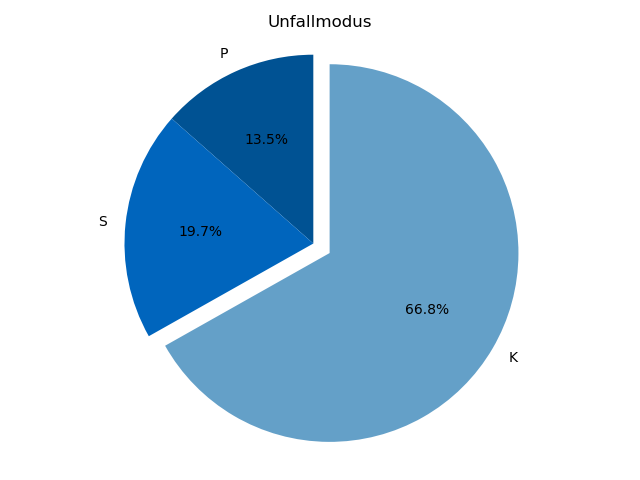
\includegraphics[width=8.1cm,height=6cm]{figures/Unfallmodus}
		\caption[Häufigkeit des Unfallmoduses]{Häufigkeit von Unfällen mit Personenschaden, Unfällen mit schwerwiegendem Sachschaden und von Kleinunfällen}\label{fig:Unfallmodus}
	\end{figure}
\end{savenotes}

\subsection{Vorstellung der Teststrecke}\label{subsechtion:Vorstellung der Teststrecke}
Um einen Überblick über die Teststrecke zu bekommen, wird diese zunächst mit dem Fokus auf Eigenschaften, die für die Datenauswertung relevant sind, analysiert. Die gewonnenen Ergebnisse sind in~\autoref{tab:teststecke} stichpunktartig dargestellt. 

\begin{table}[htpb]
	\scriptsize
	\caption[Analyse der Teststrecke im Münchner Norden]{Analyse der Teststrecke im Münchner Norden}\label{tab:teststecke}
	\centering
	\begin{tabular}{l p{3cm} p{3cm} p{3cm}}
		\toprule
		Eigenschaften & Ungererstraße & Leopoldstraße & Schenkendorfstraße \\
		\midrule
		Länge & 1,3 km & 1,5 km & 1,2 km \\
		Kreuzungen mit LSA & 3 & 2 & 2 \\
		Einmündungen mit LSA & 1 & 5 & - \\
		Einmündungen ohne LSA & 12 & 5 & 2 \\
		Abfahrten/Auffahrten & - & - & 7 \\
		Zulässige Geschwindigkeit & 50 km/h & 50 km/h & 60 km/h \\%evtl. nochmals überprüfen.
		ÖPNV Haltestellen & 2 & 3 & - \\
		Fahrspuren je Richtungsfahrbahn & 2 & 2 teilw. 3 & 2 teilw. 4 \\
		Fahrbahntrennung & durchgängiger Grünstreifen & Tram/Grünstreifen & Grünstreifen/bauliche Trennung\\
		Parkplätze im Seitenraum & Längsparkplätze & Längsparkplätze & - \\
		weitere Parkplätze & Parkplatz Münchner Freiheit & Parkhaus Schwabinger Tor & - \\
		Häufig besuchte Punkte & 2 Tankstellen & 2 Tankstellen & Tankstelle\\
		& Ungererbad & 4 Hotels & \\
		& Spielplatz & Discounter & \\
		\bottomrule
	\end{tabular}
\end{table}

Bei den Untersuchungen wurden nur die Abschnitte der drei Straßen betrachtet, die im Testgebiet liegen. Abbildung \ref{fig:Knoten_Testgebiet} in Anhang \ref{chapter:Übersichtskarten} stellt die Teststrecke und alle Knotenpunkte, unterteilt nach Kreuzungen mit LSA und Einmündungen mit/ohne LSA, dar. Kreuzungen ohne LSA kommen auf der Strecke nicht vor und werden deshalb nicht berücksichtigt. Die Knotenpunkte, welche zwei Straßen der Teststrecke verknüpfen, werden in~\autoref{tab:teststecke} doppelt gezählt. Unter Abfahrten/Auffahrten sind planfreie Knoten im Gebiet zu verstehen. Ein Beispiel stellt die Auffahrt auf die A9 Richtung Berlin von der Schenkendorfstraße aus dar. Als Fahrspuren wurden die Spuren gezählt, die über einen längeren Bereich durchgehend vorhanden sind. Im Bereich von Knotenpunkten können diese aufgeweitet werden. Teilweise ändert sich die Zahl der Spuren auch mit dem Straßenverlauf. Betrachtet man beispielsweise den südlichen Teil der Leopoldstraße, sind zwei Fahrspuren je Richtungsfahrbahn vorhanden und in der Mitte der Straße verläuft ein Rasengleis für die Tram. Die Tram wird allerdings nur bis zum Schwabinger Tor auf der Leopoldstraße geführt, danach biegt sie ab. Hier ändert sich die Anzahl der Fahrspuren von zwei auf drei je Richtungsfahrbahn. Häufig werden auch Unfälle aufgenommen, die sich nicht direkt auf einer der drei Straßen ereigneten, sondern z.B. im Bereich einer Tankstelle, die von der Straße aus angefahren werden kann oder auf einem Parkplatz. Deshalb wurden auch solche Punkte bei der Analyse des Gebiets berücksichtigt.

Bei den Kreuzungen und Einmündungen mit LSA soll zusätzlich noch berücksichtigt werden, ob Abbiegestreifen vorhanden sind und ob diese, falls vorhanden, eine eigene Signalisierung für Links- bzw. Rechtsabbieger besitzen. Im Folgenden werden deshalb diese Knotenpunkte noch detaillierter betrachtet. Die jeweiligen Knotenpunktarme sind annähernd rechtwinklig zueinander und werden deshalb in den Abbildungen in diesem Kapitel immer rechtwinklig zueinander dargestellt.

\subsubsection{Kreuzungen mit LSA}
Es gibt fünf lichtsignalisierte Kreuzungen im Testgebiet. Zwei davon besitzen keine getrennten Abbiegestreifen und werden in diesem Kapitel nicht näher erläutert. Der Knotenpunkt Rheinstraße-Leopoldstraße besitzt an allen Zufahrten einen Abbiegestreifen, hierbei handelt es sich, wie in Abbildung \ref{fig:Rhein_Leo} zu erkennen ist, um drei Linksabbiegestreifen und einen Rechtsabbiegestreifen. Es gibt jedoch keine eigene Signalisierung für einen der Abbiegestreifen. 

\begin{savenotes}
	\begin{figure}[H]
		\centering
		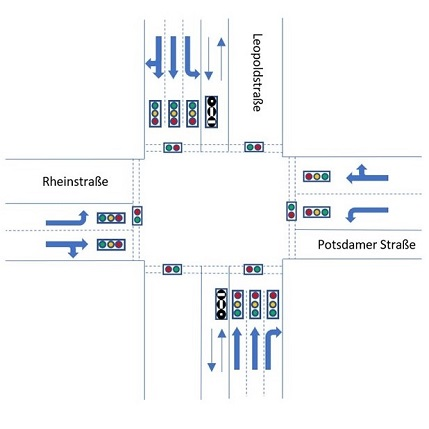
\includegraphics[width=6cm,height=6cm]{figures/Rhein_Leo}
		\caption[Kreuzung Rheinstraße-Leopoldstraße]{Kreuzung Rheinstraße-Leopoldstraße \parencite[S. 28]{Kutsch.05.04.2018}}\label{fig:Rhein_Leo}
	\end{figure}
\end{savenotes}

Die Knotenpunkte Schenkendorfstraße-Ungererstraße und Schenkendorfstraße-Leopoldstraße besitzen dagegen nicht nur mehrere Abbiegestreifen wie in Abbildung \ref{fig:eigene_Signalisierung}
gut zu erkennen ist, sondern teilweise auch eigene Signalphasen für die Abbiegespuren. Diese werden durch Pfeilsymbole an den Ampeln dargestellt. Ein Beispiel für Rechtsabbieger zeigt sich an der Kreuzung Schenkendorfstraße-Leopoldstraße. Wird die Leopoldstraße in Richtung Norden befahren ist beim Rechtsabbiegen auf die Schenkendorfstraße eine eigene Signalisierung vorhanden. Eine eigene Signalisierung für Linksabbieger existiert dagegen an der Kreuzung Schenkendorfstraße-Ungererstraße, wenn man die Ungererstraße in Richtung Norden befährt und nach links auf die Schenkendorfstraße abbiegt.

\begin{savenotes}
	\begin{figure}[H]
		\centering
		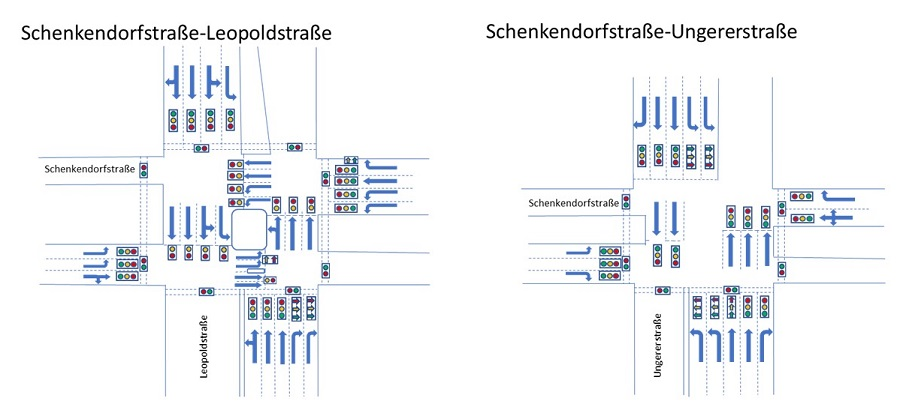
\includegraphics[width=12cm,height=6cm]{figures/Kreuzungen_eigene_Abbiegephase}
		\caption[Kreuzungen mit eigener Signalisierung für Links- bzw. Rechtsabbieger]{Kreuzung mit eigener Signalisierung für Links- bzw. Rechtsabbieger \parencite[S. 30f]{Kutsch.05.04.2018}}\label{fig:eigene_Signalisierung}
	\end{figure}
\end{savenotes}

\subsubsection{Einmündungen mit LSA}
Innerhalb des betrachteten Gebiets gibt es fünf lichtsignalgeregelte Einmündungen. Eine davon ist die Kreuzung mit der Tram am Schwabinger Tor. Der Kfz-Verkehr kann hier nicht die Richtung wechseln, er folgt weiterhin der Leopoldstraße. Eine weitere Einmündung besitzt keinen Abbiegestreifen und wird deshalb hier nicht weiter betrachtet. An der Einmündung Leopoldstraße-Ungererstraße gibt es in jedem Knotenpunktarm einen Abbiegestreifen, davon zwei für Linksabbieger und einen für Rechtsabbieger. Diese werden in Abbildung \ref{fig:Einmüngung_Abbiegestreifen} dargestellt.

\begin{savenotes}
	\begin{figure}[H]
		\centering
		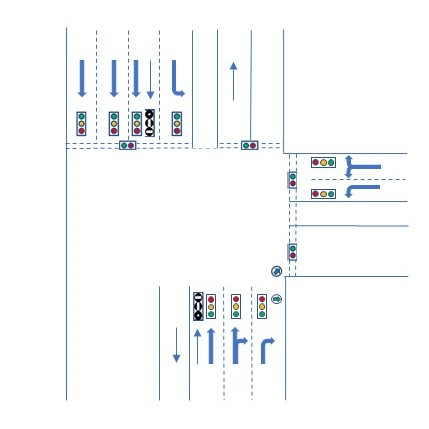
\includegraphics[width=6cm,height=6cm]{figures/Einmuendung_Abbiegestreifen}
		\caption[Einmündung Leopoldstraaße-Ungererstraße]{Einmündung Leopoldstraße-Ungererstraße \parencite{Kutsch.05.04.2018}}\label{fig:Einmüngung_Abbiegestreifen}
	\end{figure}
\end{savenotes}

Einmündungen mit einer eigenen Signalphase für Abbieger stellen die Einmündungen Johann-Fichte-Straße-Leopoldstraße und Parzivalstraße-Leopoldstraße in Abbildung \ref{fig:Einmüngungen_eigene_Phase} dar. Die Einmündung Johann-Fichte-Straße-Leopoldstraße hat einen Rechtsabbiegestreifen ohne eigene Signalisierung und einen Linksabbiegestreifen mit eigener Signalisierung. An der Parzivalstraße gibt es ebenfalls einen Linksabbiegestreifen mit eigener Signalisierung.  

\begin{savenotes}
	\begin{figure}[H]
		\centering
		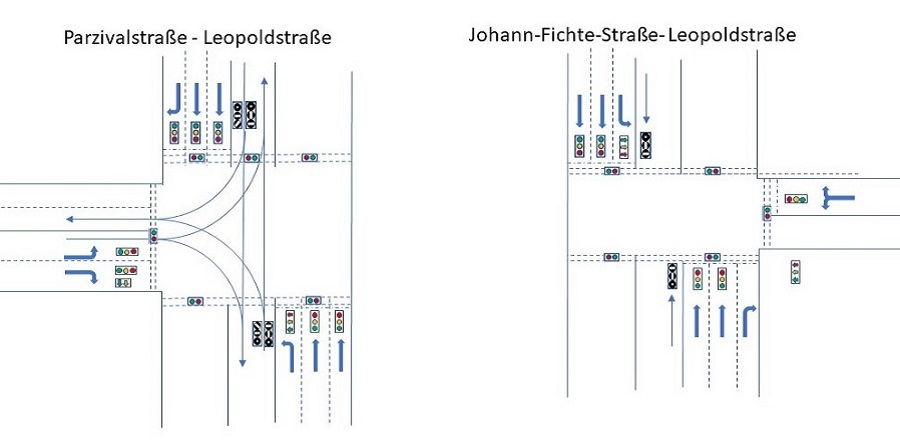
\includegraphics[width=12cm,height=6cm]{figures/Einmuendungen_eigene_Phase}
		\caption[Einmündungen mit eigener Signaphase für Abbieger]{Einmündungen mit eigener Signalphase für Abbieger \parencite{Kutsch.05.04.2018}}\label{fig:Einmüngungen_eigene_Phase}
	\end{figure}
\end{savenotes}

Bis jetzt wurden nur die Knotenpunktbereiche in Nähe der Haltelinien berücksichtigt. Im Bereich der Knotenpunktzufahrt kommt es allerdings ebenfalls häufig zu Konflikten, da hier vermehrt Spurwechsel und Bremsmanöver auftreten. \Textcite[S. 19]{Erke.1978} unterteilt die Knotenzufahrt deshalb in drei Segmente, die dann in den Knoteninnenbereich übergehen. Segment 1 beginnt 100 bis 250 m vor dem Knoten mit dem Vorwegweiser und endet mit dem Beginn der Spuraufweitung. Segment 2 erstreckt sich vom Beginn der Spuraufweitung bis zu dem Punkt, an dem alle Spuren voll ausgebildet sind. Segment 3 schließt sich an und reicht bis zur Haltelinie.

\subsection{Vorstellung der vorhandenen Daten}
Die vorhandenen Unfalldaten für das Testgebiet über die Jahre 2012 bis 2016 beinhalten allgemeine Informationen zu Datum, Uhrzeit und Position des Unfalls. Die Position wird anhand von Geographischen Koordinaten genau angegeben. Zusätzlich werden noch der Straßenname und die Hausnummer, bzw., falls es sich um einen Knotenpunkt handelt, die Namen beider Straßen genannt. Die Fahrtrichtung der Fahrzeuge wird, auf die Hausnummern bezogen, mit absteigend oder aufsteigend angegeben.

Um genauere Informationen über die Eigenschaften der Unfallstelle zu bekommen, können Charakteristiken und Besonderheiten angegeben werden. Diese Möglichkeit wurde bei den vorhandenen Daten jedoch eher selten genutzt. Ebenso dienen Angaben zu den Lichtverhältnissen, zum Straßenzustand und zu Geschwindigkeitsbeschränkungen dazu, mehr Informationen über Unfallmerkmale zu erhalten.

Zur besseren Klassifikation der Unfälle wird ihnen ein Unfallmodus zugeordnet. Es wird hierbei zwischen drei Unfallmodi unterschieden: Personenschaden, Sachschaden und Kleinunfall. Die dazugehörenden Definitionen können Kapitel \ref{subsection:Unfallfolgen} entnommen werden. Neben dem Unfallmodus Personenschaden wird noch angegeben, wie viele Personen sich bei einem Unfall leicht oder schwerverletzt haben bzw. wie viele getötet wurden. Ebenso wird die Höhe des gesamten Sachschadens angegeben.

Weitere Informationen erhält man durch die Angabe des Unfalltyps, der Unfallart und der Unfallursache. Diese wurden in Kapitel \ref{subsection:Begriffe der Unfallaufnahme} definiert. Zusätzlich wird vermerkt, wie viele Personen an einem Unfall beteiligt waren, ob sie unter Drogen- oder Alkoholeinfluss standen und ob es zu einer Unfallflucht kam. 

Für die Beteiligten wird angegeben, in welcher Art sie am Unfall beteiligt waren z.B. Hauptverursacher, welche Verletzungen sie erlitten haben und welche persönliche Unfallursache vorliegt. Dies ist notwendig, da nicht nur beim Hauptverursacher ein fehlerhaftes Verhalten vorliegen kann.

Bei den vorhandenen Daten wurden selten zu allen oben genannten Punkten Angaben gemacht. Der Datensatz weist daher zum Teil Lücken auf. Bei Kleinunfällen sind nur Angaben zu Datum, Uhrzeit, Position und allgemeiner Unfallursache gegeben. Eigenschaften, die für den späteren Vergleich mit automatisierten Fahrzeugen in  Kapitel \ref{chapter:automatisiertes Fahren} nicht relevant sind, wurden zum Teil vernachlässigt. Es wird im Verlauf der Arbeit nicht weiter darauf eingegangen, ob Fahrer unter Drogen- oder Alkoholeinfluss standen und ob es bei dem Unfall zu einer Unfallflucht kam.

\section{Allgemeine Auswertung der Daten}
Um einen Überblick über das Unfallgeschehen innerhalb des Testgebiets zu erhalten, werden zunächst nur die Unfälle betrachtet, bei denen es zu einem Personen- oder Sachschaden kam. Da für Kleinunfälle weitaus weniger Informationen vorliegen, werden diese erst im späteren Verlauf der Arbeit berücksichtigt.

Für eine erste Kategorisierung der Unfälle ist der Unfalltyp ausreichend. Dieser gibt Auskunft über die Konfliktsituation. Für die Arbeit von \Textcite[S. 16-33]{Bruhn.2018} lagen die Daten des Testgebiets ebenfalls vor. Er hat Karten erstellt, in denen die Unfälle der verschiedenen Unfalltypen auf der kompletten Länge der drei Straßen im Testgebiet abgebildet werden. Neben der Lage wurden auch die Schwere der Verletzungen und die Hauptverursacher der Unfälle analysiert. In Abbildung \ref{fig:Unfalltyp} wird deshalb nur ein Überblick über die  Anzahl der Unfälle mit zugehörigem Unfalltyp und Unfallmodus innerhalb des betrachteten Zeitraums gegeben. Da hier nur der Bereich der Straßen innerhalb des Testgebiets betrachtet wurde, weichen die Ergebnisse zum Teil von denen von \Textcite[S. 16-33]{Bruhn.2018} ab. 

Am zweithäufigsten wurde nach dem Unfalltyp 7 \enquote{Sonstiger Unfall} der Typ 6 \enquote{Unfall im Längsverkehr} bei 26 \% der Unfälle angegeben. Hierbei kam es bei 45 \% der Unfälle zu einem Personenschaden. Am dritthäufigsten ereigneten sich Unfälle mit dem Unfalltyp 2 \enquote{Abbiege-Unfall}. Hierbei kam es in 60 \% zu Unfällen mit Personenschaden. 13 \% der Unfälle wiesen den Unfalltyp 3 \enquote{Einbiegen/Kreuzen-Unfall} auf. Bei diesem Typ handelt es sich an der Einmündung Schenkendorfstraße/Lyonel-Feininger-Straße laut \Textcite[S. 23]{Bruhn.2018} um eine kritische Stelle. Unfälle des Typs 4 \enquote{Überschreitunfälle} kommen zwar selten vor, führten aber immer zu einem Personenschaden und ereigneten sich überwiegend in der Leopoldstraße. Hierbei sind vor allem die Bereiche auffällig, in denen sich die Tramhaltestellen in der Mitte der Fahrbahn befinden. Alle Unfälle mit Todesfolge gehörten zu diesem Unfalltyp \parencite[S. 26f]{Bruhn.2018}. Bei dem Typ 5 \enquote{Unfall des ruhenden Verkehrs} kam es dagegen lediglich in 13 \% der Unfälle zu einem Personenschaden.

\begin{savenotes}
	\begin{figure}[H]
		\centering
		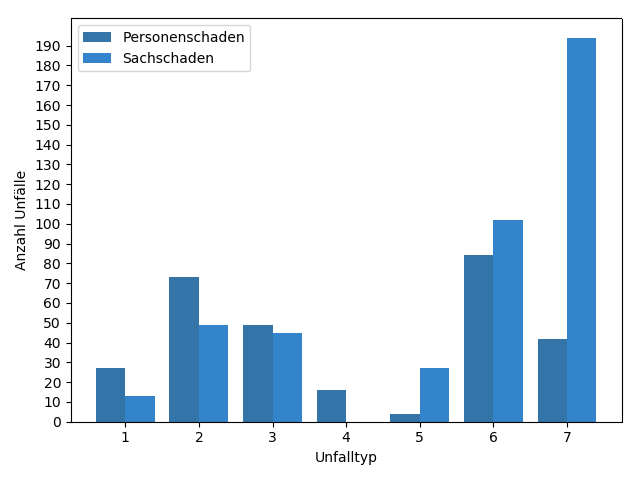
\includegraphics[width=8cm,height=6cm]{figures/Unfalltyp}
		\caption[Unfalltyp der Unfälle, die in den Jahren 2012 bis 2016 im Testgebiet aufgenommen wurden]{Unfalltyp der Unfälle, die in den Jahren 2012 bis 2016 im Testgebiet aufgenommen wurden}\label{fig:Unfalltyp}
	\end{figure}
\end{savenotes}

Die Unfallart wird herangezogen, um die Bewegungsrichtung der Fahrzeuge während des Unfalls zu beschreiben. Unfällen, bei denen ein Personen- oder Sachschaden entstand, wurde eine Unfallart zugeordnet. Innerhalb des Testgebiets kam es am häufigsten zu Unfällen, bei denen die Unfallart 1 \enquote{Zusammenstoß mit Fahrzeug, das anfährt, anhält oder im ruh. Verkehr steht} angegeben wurde. Bei 26 \% der aufgenommenen Unfälle wurde die Unfallart 1 angegeben, bei 22 \% die Unfallart 5 \enquote{Zusammenstoß mit Fahrzeug, das einbiegt oder kreuzt}. Während es bei Unfällen mit der Unfallart 1 größtenteils nur zu einem Sachschaden kam, hatten mehr als die Hälfte mit der Unfallart 5 einen Personenschaden zur Folge. Am dritthäufigsten ereigneten sich Unfälle mit der Unfallart 3 \enquote{Zusammenstoß mit Fahrzeug, das seitlich oder in gleicher Richtung fährt}. Hierbei kam es in 72 \% lediglich zu einem Sachschaden. Die Unfallart 6 \enquote{Zusammenstoß zwischen Fahrzeug und Fußgänger} wurde zwar nur bei 4 \% der Unfälle angegeben, es ergab sich jedoch immer ein Personenschaden. Abbildung \ref{fig:Unfallart} gibt einen Überblick über die Unfallarten und die Unfallschwere, die den Unfällen im Testgebiet zugeordnet wurden.

\begin{savenotes}
	\begin{figure}[H]
		\centering
		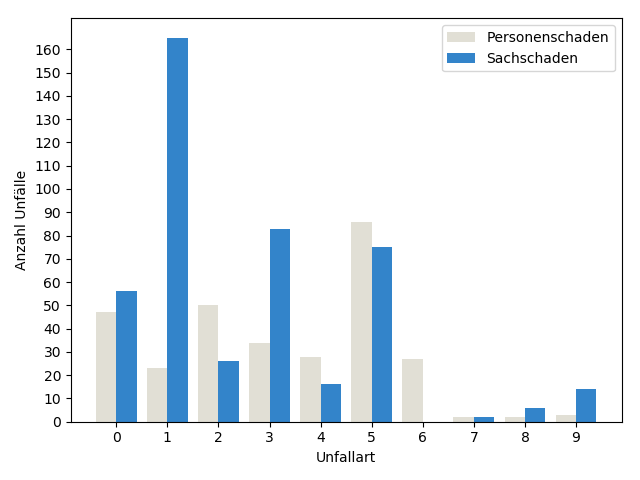
\includegraphics[width=8cm,height=6cm]{figures/Unfallart}
		\caption[Unfallart der Unfälle, die in den Jahren 2012 bis 2016 im Testgebiet aufgenommen wurden]{Unfallart der Unfälle, die in den Jahren 2012 bis 2016 im Testgebiet aufgenommen wurden}\label{fig:Unfallart}
	\end{figure}
\end{savenotes}

Die \ac{BArt} gibt Auskunft darüber, ob ein Unfallbeteiligter Hauptverursacher (BArt01) oder Geschädigter ist (BArt02/BArt03). Innerhalb des Testgebiets wurden nur Unfälle mit bis zu drei Unfallbeteiligten aufgenommen. Die Beteiligungsart wurde nur bei Unfällen angegeben, bei denen Personen- oder Sachschaden entstand. In 63 \% handelte es sich bei den Hauptverursachern um Pkw-Fahrer. Am zweithäufigsten wurden Unfälle durch unbekannte Fahrzeuge (13 \%) ausgelöst, unbekannt wird meistens bei Unfällen mit Fahrerflucht angegeben. An dritter Stelle stehen Lkw-Fahrer mit 10 \% als Hauptverursacher. Bei den Unfallgegnern machten ebenfalls die Pkw-Fahrer mit 71 \% den größten Anteil aus. An zweiter Stelle stehen Fahrradfahrer mit 16 \%. In Abbildung \ref{fig:Beteiligungsart} werden die Unfälle im Testgebiet nach Beteiligungsart und Art der Verkehrsbeteiligung dargestellt. 

\begin{savenotes}
	\begin{figure}[H]
		\centering
		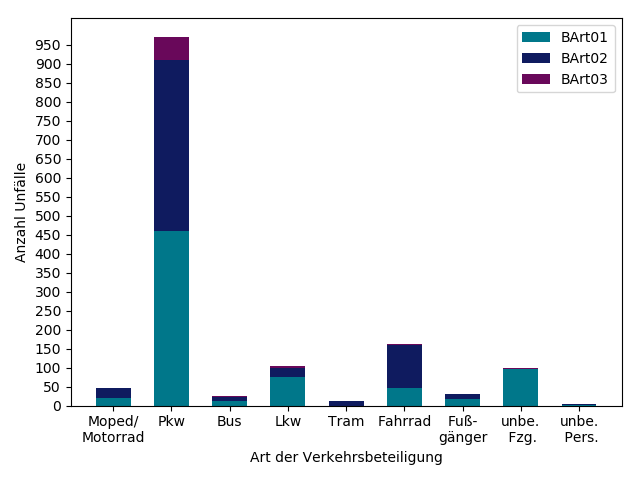
\includegraphics[width=8cm,height=6cm]{figures/BArt}
		\caption[Beteiligungsart der Verkehrsteilnehmer, die bei Unfällen in den Jahren 2012 bis 2016 im Testgebiet angegeben wurden]{Beteiligungsart der Verkehrsteilnehmer, die bei Unfällen in den Jahren 2012 bis 2016 im Testgebiet angegeben wurden}\label{fig:Beteiligungsart}
	\end{figure}
\end{savenotes}

\section{Überprüfung der Hypothesen}\label{sechtion:Überprüfung der Thesen}
In diesem Kapitel werden die in Kapitel \ref{chapter:Methodik} aufgestellten Hypothesen auf ihre Gültigkeit hin überprüft. Da zu vermuten ist, dass die Genauigkeit der Unfallaufnahme mit der Schwere der Unfallfolgen ansteigt und somit die Daten von Personenschadensunfällen verlässlicher sind \parencite[S. 11]{StatistischesBundesamt.2018b}, wird bei der statistischen Auswertung der vorhandenen Unfalldaten der Unfallmodus mit einbezogen. Dieser gibt an, ob es sich um Unfälle mit Personen- bzw. Sachschaden oder um Kleinunfälle handelt. Zusätzlich wird in den meisten Fällen nach bestimmten Unfallursachen differenziert, um den Unfallhergang möglichst genau abzubilden. %Kann man das so als Einleitung stehen lassen?

\subsection{Abbiegeunfälle}\label{subsechtion:Abbiegeunfälle}
Der Unfalltyp Abbiegeunfälle wurde bei insgesamt 17 \% der Unfälle im Untersuchungsgebiet mit Personen- oder Sachschaden angegeben. Dabei kam es in 60 \% zu Unfällen mit Personenschaden, siehe Abbildung \ref{fig:Unfallart}. Der Unfalltyp gibt jedoch keine Auskunft, ob es sich um einen Unfall beim Rechtsabbiegen oder Linksabbiegen handelt. Hierfür werden zusätzlich die Unfallursachen \enquote{Fehler beim Abbiegen nach rechts} (34) und \enquote{Fehler beim Abbiegen nach links} (35) betrachtet. Abbildung \ref{fig:Abbiegen_rechts_links} zeigt das Verhältnis der Unfälle, bei denen eine der beiden Ursachen angegeben wurde. Innerhalb des betrachteten Zeitraums ereigneten sich 57,7 \% der Unfälle beim Abbiegen nach links und bilden somit die Mehrheit der Abbiegeunfälle.

\begin{savenotes}
	\begin{figure}[H]
		\centering
		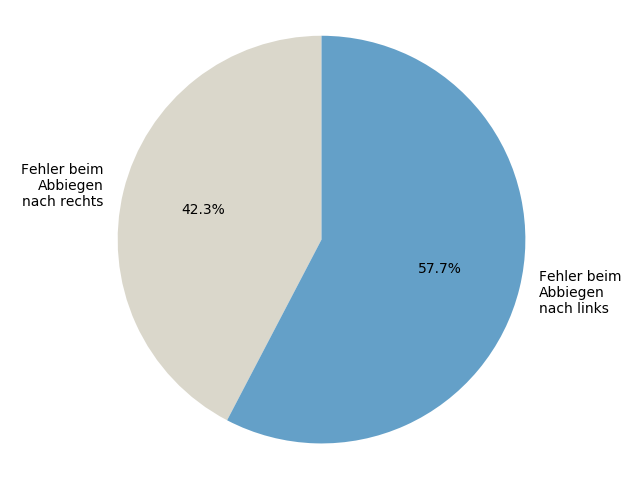
\includegraphics[width=8cm,height=6cm]{figures/These_1}
		\caption[Unfälle bei denen Abbiegefehler nach rechts bzw. links in den Jahren 2012 bis 2016 im Testgebiet aufgenommen wurden]{Unfälle bei denen Abbiegefehler nach rechts bzw. links in den Jahren 2012 bis 2016 im Testgebiet aufgenommen wurden}\label{fig:Abbiegen_rechts_links}
	\end{figure}
\end{savenotes}

Berücksichtigt wurden alle Unfälle, unabhängig vom Unfalltyp, denen entweder die \ac{Urs} 34 oder 35 zugeordnet wurde. Somit können auch Kleinunfälle, denen kein Unfalltyp zugeordnet wurde, berücksichtigt werden. Abbildung \ref{fig:Abbiegen_Md} stellt die Anzahl der Unfälle beim Abbiegen nach links bzw. rechts und den zugehörigen Unfallmodus dar. Vor allem beim Abbiegen nach links kommt es häufig nur zu Kleinunfällen.
Bei der Mehrheit der Unfälle mit Sach- und Personenschaden wurde auch der Unfalltyp 2 angegeben, bei Urs34 in 83 \% bei Urs35 in 76 \% der Fälle.

\begin{savenotes}
	\begin{figure}[H]
		\centering
		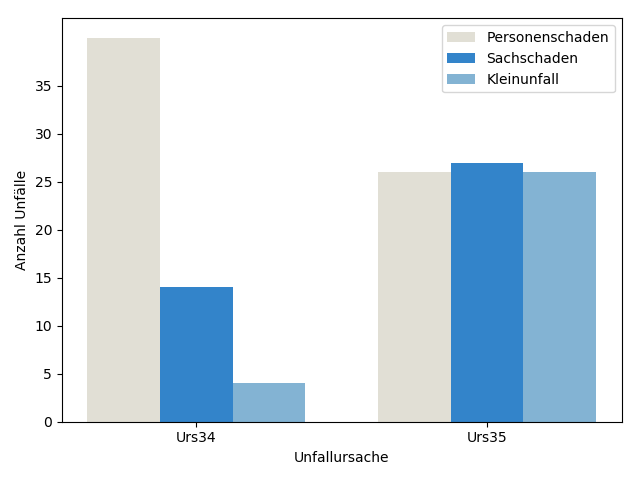
\includegraphics[width=8cm,height=6cm]{figures/Abbiegen_Md}
		\caption[Unfallmodus bei Abbiegeunfällen, die in den Jahren 2012 bis 2016 im Testgebiet aufgenommen wurden]{Unfallmodus bei Abbiegeunfällen, die in den Jahren 2012 bis 2016 im Testgebiet aufgenommen wurden}\label{fig:Abbiegen_Md}
	\end{figure}
\end{savenotes}

Unfälle beim Rechtsabbiegen sind zwar seltener, dafür kommt es zu schwereren Verletzungen. Häufig wird hierbei, wie in Abbildung \ref{fig:Abbiegen_Verletzungen} dargestellt ist, nicht der Hauptverursacher des Unfalls sondern der zweite Unfallbeteiligte verletzt. Dies liegt daran, dass es oft zu Unfällen zwischen Pkw-Fahren und Fahrradfahren kommt, vgl. Kapitel \ref{subsection:Abbiegeunfälle mit Radfahrern}. Beim Abbiegen nach links ist die Verletzungsschwere geringer, da sich viele Unfälle zwischen zwei Pkws ereignen. \textit{Hypothese 1} behauptet, dass es beim Linksabbiegen mehr Konfliktpunkte gibt und es daher häufiger zu Unfällen kommt als beim Rechtsabbiegen und kann anhand der oben genannten Zahlen bestätigt werden.

\begin{savenotes}
	\begin{figure}[H]
		\centering
		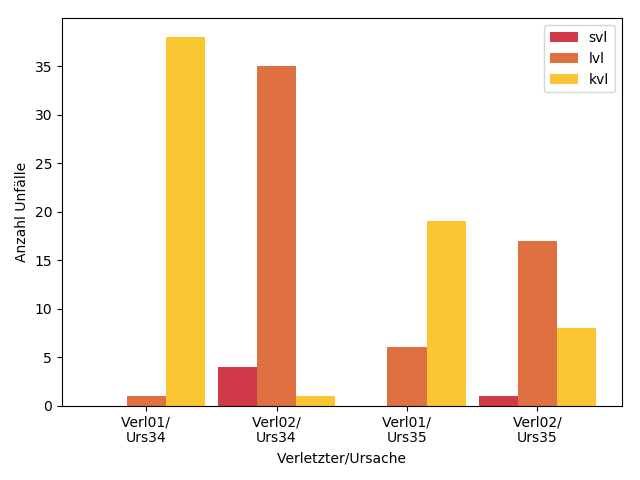
\includegraphics[width=8cm,height=6cm]{figures/Abbiegen_Verletzung}
		\caption[Verletzungsschwere der Unfallbeteiligten bei Abbiegeunfällen, die in den Jahren 2012 bis 2016 im Testgebiet aufgenommen wurden]{Verletzungsschwere bei Abbiegeunfällen, die in den Jahren 2012 bis 2016 im Testgebiet aufgenommen wurden}\label{fig:Abbiegen_Verletzungen}
	\end{figure}
\end{savenotes}

In Abbildung \ref{fig:map_Urs35} sind Orte markiert, an denen Unfälle durch Fehler beim Linksabbiegen entstanden sind. Auffällig sind hier vor allem die Knotenpunkte Leopoldstraße/Potsdamer Straße, Schenkendorfstr./Ungererstr. und Leopoldstr./Ungererstraße. Die Knotenpunkte wurden bereits in Kapitel \ref{subsechtion:Vorstellung der Teststrecke} genauer beschrieben. Anhand der Kurzsachverhalte kann man bei fast allen Unfällen auf den genauen Unfallhergang schließen. An der Kreuzung Leopoldstr./Potsdamer Str. ereigneten sich innerhalb der Jahre 2013 bis 2016 insgesamt 16 Unfälle zwischen einem Fahrzeug, das die Leopoldstr. in südlicher Richtung befuhr und nach links in die Potsdamer Straße abbiegen wollte und einem Fahrzeug, welches die Leopoldstr. geradeaus in nördliche Richtung befuhr. Bei sechs der aufgenommenen Unfälle handelte es sich beim Unfallgegner um Radfahrer. Zusätzlich kam es zu vier Unfällen zwischen Linksabbiegern und einer nachfolgenden Tram. In Abbildung \ref{fig:Rhein_Leo} ist zu erkennen, dass die Kreuzung zwar einen Linksabbiegestreifen besitzt, dieser wird jedoch nicht durch eine eigene Signalphase geregelt. Deshalb kommt es häufig zu Konflikten mit entgegenkommenden Fahrzeugen.

\begin{savenotes}
	\begin{figure}[H]
		\centering
		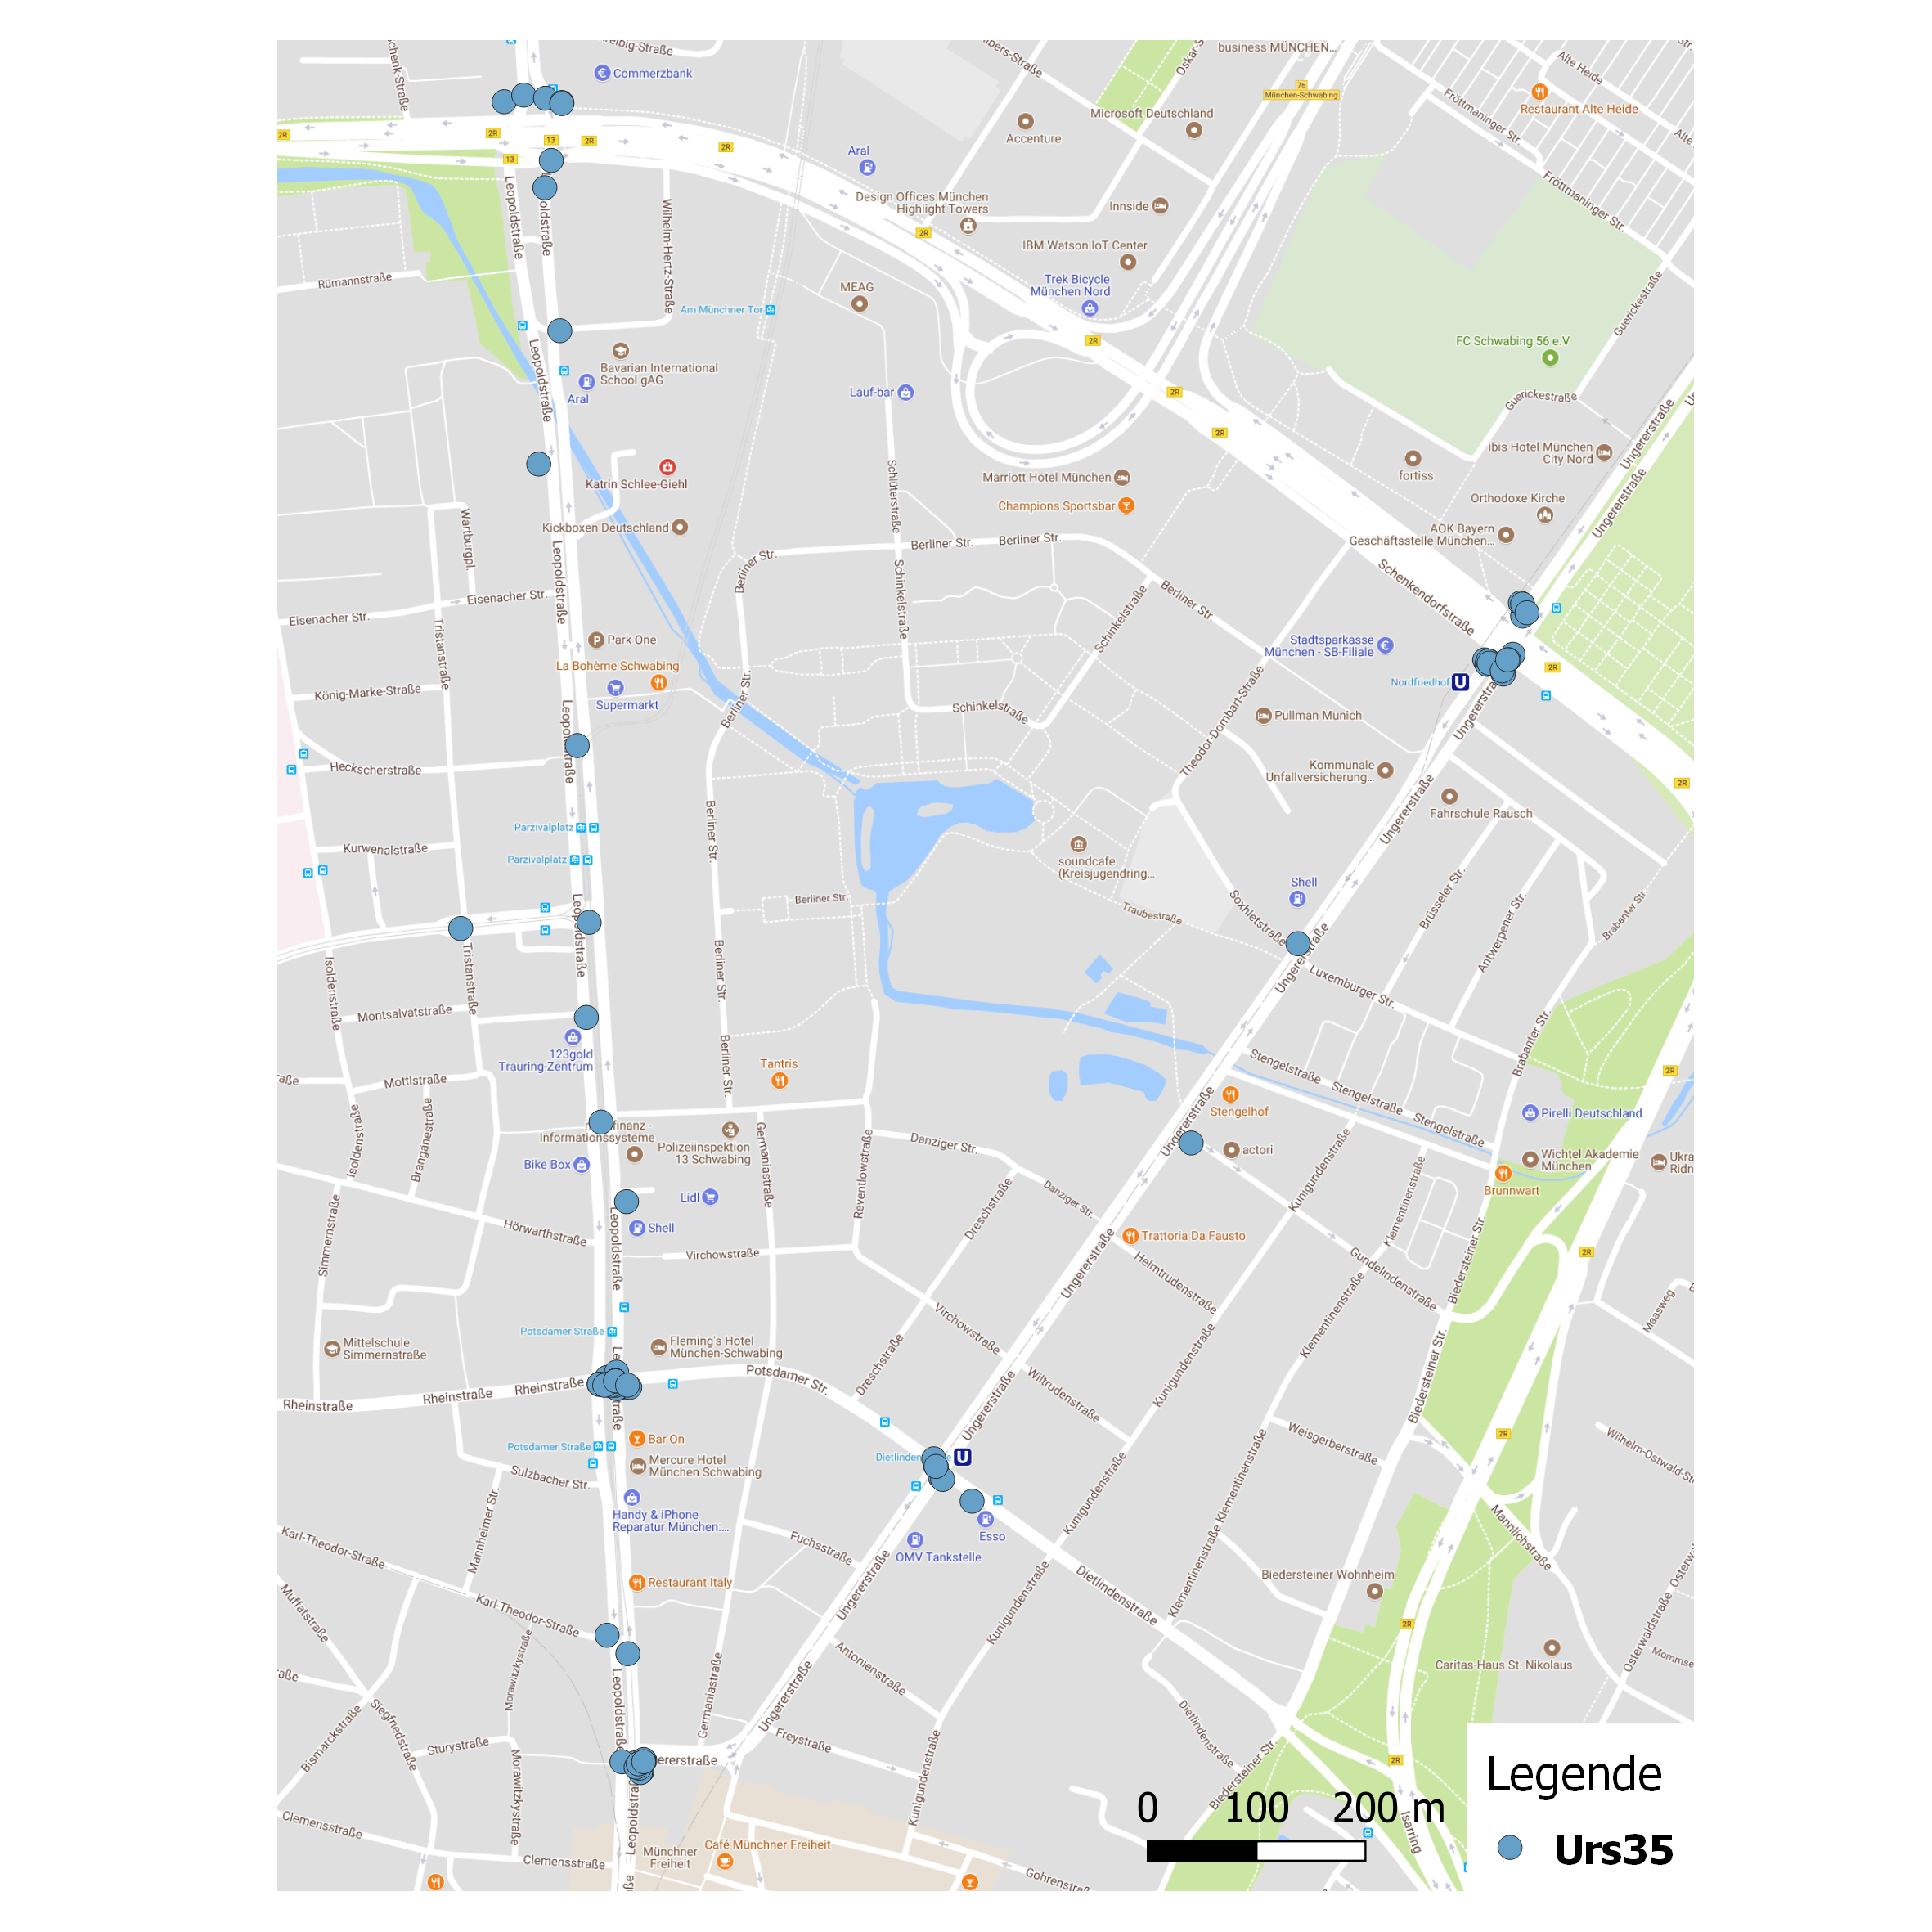
\includegraphics[width=10cm,height=10cm]{figures/map_Urs35}
		\caption[Unfälle durch Fehler beim Linksabbiegen, die in den Jahren 2012 bis 2016 im Testgebiet aufgenommen wurden]{Unfälle durch Fehler beim Linksabbiegen, die in den Jahren 2012 bis 2016 im Testgebiet aufgenommen wurden}\label{fig:map_Urs35}
	\end{figure}
\end{savenotes}

Die Kreuzung Ungererstraße/Schenkendorfstraße besitzt Linksabbiegestreifen mit eigener Signalphase (Abbildung  \ref{fig:eigene_Signalisierung}). Eine Phase ist für die Ungererstr. in südliche Fahrtrichtung und eine für die Ungererstr. in nördliche Fahrtrichtung. Trotzdem sieht es so aus, als würden sich an dieser Kreuzung ähnlich viele Unfälle ereignen, wie an der zuvor diskutierten. Betrachtet man die Unfälle genauer, handelt es sich vor allem um Unfälle mit Fahrzeugen, die in die gleiche Richtung fahren. Die Linksabbieger werden auf zwei Linksabbiegestreifen nebeneinander geführt. Kommt ein Fahrzeug beim nebeneinander Abbiegen von der Fahrbahn ab, kann es zu einem Unfall mit dem zweiten abbiegenden Fahrzeug kommen. Zu Unfällen mit entgegenkommenden Fahrzeugen kam es an dieser Kreuzung nur in vier Fällen. Ursache hierfür waren nicht verkehrsgerechte Wendemanöver.

Die Einmündung Leopoldstraße/Ungererstraße besitzt keine eigene Signalphase für Linksabbieger (Abbildung \ref{fig:Einmüngung_Abbiegestreifen}). Hier ereigneten sich in den Jahren 2013 bis 2016 fünf Unfälle zwischen Fahrzeugen, welche den Abbiegestreifen auf der Leopoldstraße in südliche Richtung befuhren, um nach links in die Ungererstr. abzubiegen, und entgegenkommenden Fahrzeugen. An den Einmündungen mit einer eigenen Signalphase für Linksabbieger, die in der Abbildung \ref{fig:Einmüngungen_eigene_Phase} dargestellt werden, ereignete sich lediglich ein Unfall im Untersuchungszeitraum. Hierbei handelt es sich um einen Auffahrunfall, welcher durch zu starkes Bremsen beim Abbiegevorgang ausgelöst wurde.

\begin{table}[htpb]
	\scriptsize
	\caption[Verkehrsstärken an ausgewählten Linksabbiegestreifen im Testgebiet]{Verkehrsstärken an ausgewählten Linksabbiegestreifen im Testgebiet}\label{tab:Linksabbieger}
	\centering
	\begin{tabular}{l p{3cm} p{3cm} }
		\toprule
		Knotenpunkt & Linksabbiegestreifen & Verkehrsstärke [Kfz/Tag] \\
		\midrule
		Leopoldstr./Potsdamer Str. & Leopoldstr. in südl. Richtung & 2084 \\
		Leopoldstr./Parzivalstr. & Leopoldstr. in nördl. Richtung & 2027 \\
		Leopoldstr./Ungererstr. & Leopoldstr. in südl. Richtung & 2206 \\
		\bottomrule
	\end{tabular}
\end{table}

Neben den Unfällen wurden an den Knotenpunkten in der Leopoldstraße auch die Verkehrsstärken berücksichtigt. Für die Kreuzung Ungererstraße/Schenkendorfstraße liegen leider keine Werte vor. Es wurden an den Kreuzungen jeweils die Messwerte von Detektoren der Linksabbiegerstreifen betrachtet. Als Referenz wurde Donnerstag der 7.5.2016 bzw. 3.5.2018 gewählt. Hierbei handelt es sich um einen Arbeitstag außerhalb der Schulferien. Der Einfachheit halber wurde die Tagessumme der Messwerte zum Vergleich verwendet. Diese wird in Tabelle \ref{tab:Linksabbieger} für die drei Knotenpunkte dargestellt. Die Verkehrsstärken der Knoten Leopoldstr./Reihnstr. und Leopoldstr./Parzivalstr. weichen nur minimal voneinander ab. Trotzdem ereignen sich an erstgenanntem Knoten wesentlich mehr Unfälle. Die Daten für die Einmündung Ungererstr./Leopoldstr. sind aus dem Jahr 2018 und weisen eine etwas höhere Verkehrsstärke auf. Es ist anzunehmen, dass sich die Verkehrsstärke innerhalb zwei Jahren etwas erhöht hat. Die Verkehrsstärke im Jahr 2016 sollte hier also ähnlich gewesen sein, wie an den anderen zwei Knotenpunkten. Trotzdem ereigneten sich an der Einmündung mit der Ungererstraße mehr Unfälle als an der Parzivalstraße. 

\begin{savenotes}
	\begin{figure} [H]
		\subfigure{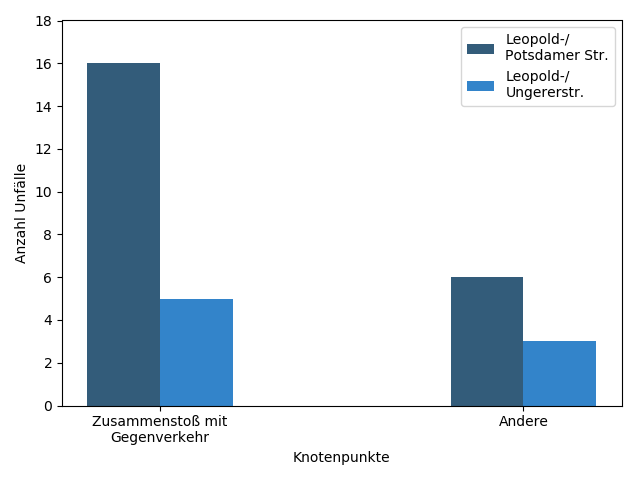
\includegraphics[width=0.49\textwidth,height=6cm]{figures/Unfaelle_Signalphasen_ohne}} 
		\subfigure{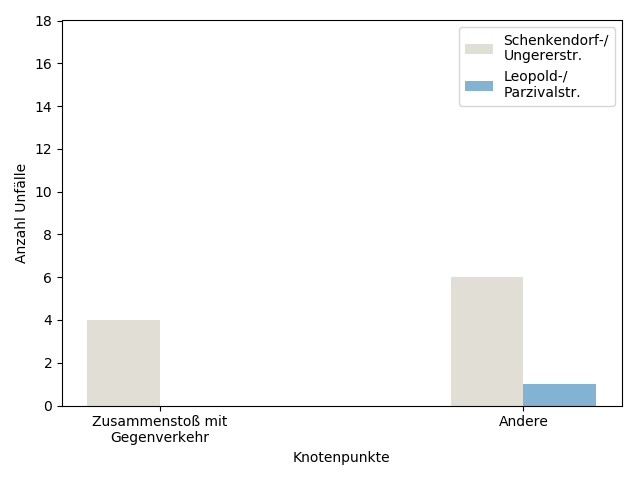
\includegraphics[width=0.49\textwidth,height=6cm]{figures/Unfaelle_Signalphasen_mit}} 
		\caption[Linksabbiegeunfälle an Knotenpunkten ohne (links) und mit (rechts) eigener Signalisierung, die in den Jahren 2013 bis 2016 im Testgebiet aufgenommen wurden]{Linksabbiegeunfälle an Knotenpunkten ohne (links) und mit (rechts) eigener Signalisierung, die in den Jahren 2013 bis 2016 im Testgebiet aufgenommen wurden}\label{fig:Unfaelle_Signalphasen} 
	\end{figure}
\end{savenotes}

\textit{Hypothese 2} gibt an, dass sich die Konfliktpunkte und Unfallzahlen reduzieren, wenn Linksabbieger an Kreuzungen mit \ac{LSA} auf einem eigenen Fahrstreifen mit eigener Signalphase geführt werden. Betrachtet man die Zahlen in Abbildung \ref{fig:Unfaelle_Signalphasen} kommt es in 73 \% der Fälle an Kreuzungen ohne eigene Signalisierung zu Unfällen beim Linksabbiegen. In 70 \%  der Fälle handelt es sich dabei um Unfälle mit entgegenkommenden Fahrzeugen. Vor allem dieser Konflikt kann durch eine eigene Phase deutlich reduziert werden. \textit{Hypothese 2} kann daher bestätigt werden.

\subsection{Unfälle während der Hauptverkehrszeiten}\label{subsechtion:Unfälle während der HVZ}
Laut Statistischem Bundesamt ereigneten sich im Jahr 2016 die meisten Unfälle innerhalb von Ortschaften, bei denen es zu einem Personenschaden kam, von Montag bis Freitag zwischen 7 und 20 Uhr. In den Morgenstunden kommt es zwischen 7 und 8 Uhr am häufigsten zu Unfällen. Auffällig ist, dass keine deutlichen Spitzen zu den vermuteten Hauptverkehrszeiten (vormittags/nachmittags) zu erkennen sind.  Die Zahl der Unfälle steigt nach einem leichten Rückgang am Vormittag schon zur Mittagszeit gegen elf Uhr wieder an. Am Nachmittag passieren die meisten Unfälle zwischen 16 und 18 Uhr. Auffällig ist auch, dass sich mehr Unfälle am Nachmittag als am Vormittag ereignen. An Wochenenden kommt es seltener zu Unfällen, dafür ist die Anzahl in den Nächten von Freitag auf Samstag und von Samstag auf Sonntag höher als unter der Woche \parencite[S. 80f]{StatistischesBundesamt.2017}.

Für das Testgebiet stehen zum Teil Messwerte von Detektoren an Knotenpunkten zur Verfügung. \Textcite[S. 10-16]{Bruhn.2018} hat anhand dieser Daten ermittelt, wann die Verkehrsmengen auf den einzelnen Straßen am höchsten sind. In der Leopoldstraße ist die Verkehrsmenge grundsätzlich von 8 bis 19 Uhr erhöht. Einzelne Spitzen sind am Vormittag zwischen 8 und 10 Uhr und abends zwischen 18 und 19 Uhr zu erkennen. Diese sind jedoch sehr gering ausgeprägt. Auf der Ungererstraße ist das Verkehrsaufkommen zwischen 7 und 9 Uhr sowie zwischen 16 und 19 Uhr erhöht. Auf der Schenkendorfstraße konnte in den Zeiträumen von 7 bis 9 Uhr und 17 bis 19 Uhr ein erhöhtes Verkehrsaufkommen festgestellt werden. Bei den Detektordaten werden nicht motorisierte Verkehrsteilnehmer vernachlässigt, da an Rad- bzw. Fußgängerüberwegen keine Detektoren vorhanden sind.

\begin{savenotes}
	\begin{figure}[H]
		\centering
		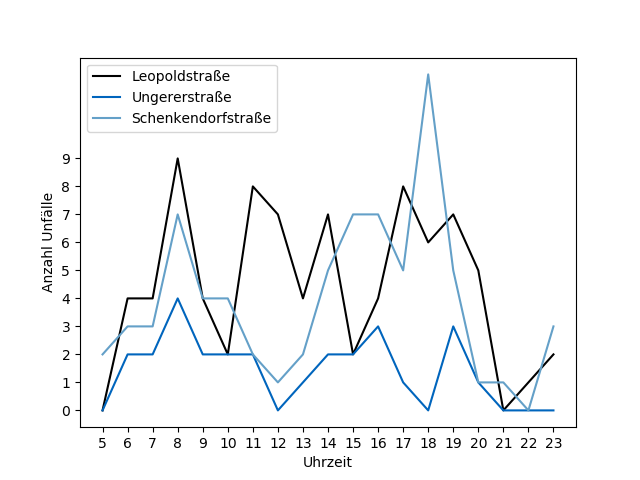
\includegraphics[width=8cm,height=6cm]{figures/Typ6}
		\caption[Zeitliche Verteilung der Unfälle mit Unfalltyp 6 in den Jahren 2012 bis 2016 innerhalb des Testgebiets]{Zeitliche Verteilung der Unfälle mit Unfalltyp 6 in den Jahren 2012 bis 2016 innerhalb des Testgebiets}\label{fig:Unfalltyp6_Uhrzeit}
	\end{figure}
\end{savenotes}

\textit{Hypothese 3} gibt an, dass bei höherem Verkehrsaufkommen die Anzahl der Verkehrsunfälle im Längsverkehr steigt. Zur Überprüfung der These werden hier nur die Unfälle betrachtet, bei denen der Unfalltyp 6 angegeben wurde. Der zeitliche Verlauf aller Unfälle im Testgebiet wurde bereits von \Textcite[S. 10-16]{Bruhn.2018} analysiert. In Abbildung \ref{fig:Unfalltyp6_Uhrzeit} ist zu erkennen, dass Unfälle im Längsverkehr auf der Leopoldstraße zwischen 8 und 20 Uhr erhöht auftraten. Auf der Ungererstraße ereigneten sich innerhalb des Untersuchungszeitraums insgesamt nur 27 Unfälle mit dem Unfalltyp 6. Daher ist es schwer, Zeitpunkte mit erhöhtem Verkehrsaufkommen zu bestimmen. Zwischen 8 und 9 Uhr, 16 und 17 Uhr sowie zwischen 19 und 20 Uhr sind leichte Spitzen zu erkennen. Auf der Schenkendorfstraße kam es vormittags zwischen 8 und 11 Uhr sowie nachmittags zwischen 14 und 20 Uhr vermehrt zu Unfällen im Längsverkehr. Am meisten Unfälle ereigneten sich zwischen 18 und 19 Uhr, hier ist in Abbildung \ref{fig:Unfalltyp6_Uhrzeit} eine deutliche Spitze zu erkennen. Vergleicht man die Zeiträume, in denen sich Unfälle ereigneten mit den Messwerten der Detektoren, stimmen diese nur zum Teil überein. Auf der Leopoldstraße wurden sowohl ein erhöhtes Verkehrsaufkommen als auch erhöhte Unfallzahlen über den gesamten Tag festgestellt. Die Unfallzahlen der Ungererstraße sind für einen konkreten Vergleich zu gering, auf der Schenkendorfstraße stimmen die Bereiche fast überein. Die Zeiträume, in denen es vermehrt zu Unfällen kommt, sind jedoch größer als diejenigen mit erhöhtem Verkehrsaufkommen. Zusammenfassend sind die Daten nicht aussagekräftig genug, um \textit{Hypothese 3} vollständig bestätigen zu können.

\begin{savenotes}
	\begin{figure}[H]
		\centering
		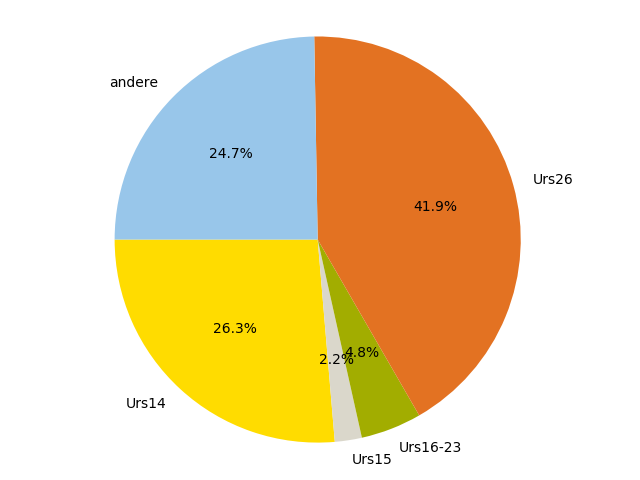
\includegraphics[width=8cm,height=6cm]{figures/Urs_Typ6}
		\caption[Unfallursachen, die Unfällen im Längsverkehr innerhalb des Testgebiets zugeordnet wurden]{Unfallursachen, die Unfällen im Längsverkehr innerhalb des Testgebiets zugeordnet wurden}\label{fig:Unfallursachen_Unfalltyp6}
	\end{figure}
\end{savenotes}

\textit{Hypothese 3} gibt zudem an, dass sich Unfälle im Längsverkehr hauptsächlich durch Konflikte beim Spurwechsel und durch zu geringen Sicherheitsabstand ereignen. Hierfür wurden die Unfallursachen betrachtet, die angegeben werden können, wenn beim Fahrzeugführer Fehler auftraten, die auf den Abstand, das Überholen oder das Nebeneinanderfahren zurückzuführen sind. Bei 75 \% der Unfälle im Längsverkehr wurde eine dieser Ursachen angegeben. Am häufigsten kam es dabei zu Unfällen aufgrund von Fehlern beim Fahrstreifenwechsel (Ursache 26). Diese Ursache wurde bei 42 \% der Unfälle mit Unfalltyp 6 angegeben. Gefolgt von der Ursache 14 \enquote{ungenügender Sicherheitsabstand}, welche bei 26 \% genannt wurde. Fehler beim Überholen wurden lediglich bei 5 \% notiert. Bei 2 \% der Unfälle wurde die Ursache 15 \enquote{Starkes Bremsen des Vorausfahrenden ohne zwingenden Grund} angegeben. Bei 46 Unfällen (25 \%) wurden Ursachen angegeben, die auf auf den ersten Blick nicht auf Unfälle im Längsverkehr hinweisen. In Abbildung \ref{fig:Unfallursachen_Unfalltyp6} werden die Unfallursachen der Unfälle im Längsverkehr angegeben. Die häufige Nennung der Unfallursachen, die auf Fehler beim Spurwechsel oder zu geringen Sicherheitsabstand hinweisen, führt dazu, dass \textit{Hypothese 3} in diesem Punkt bestätigt werden kann.

\begin{savenotes}
	\begin{figure}[H]
		\centering
		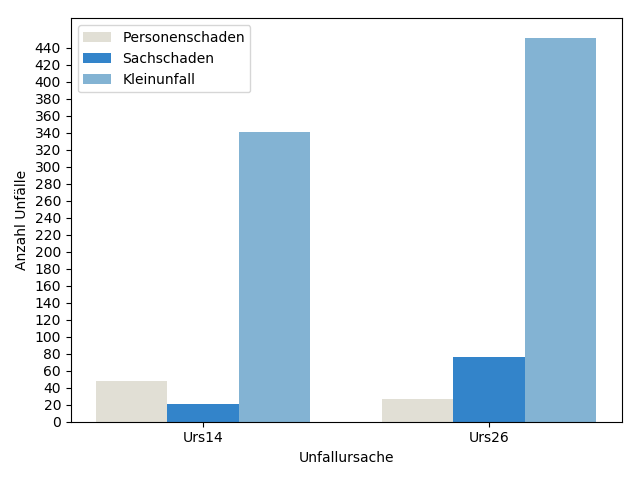
\includegraphics[width=8cm,height=6cm]{figures/Urs14_Urs26_Md}
		\caption[Schwere der Unfälle, bei denen als Unfallursache Ungenügender Sicherheitsabstand bzw. Fehler beim Spurwechsel angegeben wurden]{Schwere der Unfälle, bei denen als Unfallursache Ungenügender Sicherheitsabstand bzw. Fehler beim Spurwechsel angegeben wurden}\label{fig:Unfallursachen_14_26}
	\end{figure}
\end{savenotes}

Betrachtet man nur die Unfallursachen 14 und 26 ohne Unfalltyp können auch Kleinunfälle mit berücksichtigt werden. Diese machen, wie in Abbildung \ref{fig:Unfallursachen_14_26} zu erkennen ist, mit 83 \% bei Ursache 26 bzw. 81 \% bei Ursache 14 einen erheblichen Anteil aus. Auffällig ist zudem, dass es zwar seltener zu Unfällen durch zu geringen Sicherheitsabstand kam, diese dafür häufiger zu Personenschaden führten, als die Unfälle beim Spurwechsel.

\subsection{Unfälle durch ruhenden Verkehr}
Unfälle des ruhenden Verkehrs stellen den Unfalltyp 5 in Abbildung \ref{fig:Unfalltyp} dar. Im Untersuchungszeitraum wurden 31 Unfälle von diesem Typ aufgenommen. Bei lediglich 13 \% davon kam es zu einem Personenschaden. Ein Unfalltyp wurde nur den Unfällen mit Personen- bzw. Sachschaden zugeordnet. Bei Kleinunfällen kann man nur anhand von angegebenen Unfallursachen erkennen, ob es sich um einen Unfall durch ruhenden Verkehr handelt. Betrachtet man zunächst die Unfälle, denen ein Unfalltyp zugeordnet wurde, ereigneten sich ca. 61 \% auf der Leopoldstraße, 29 \% auf der Ungererstraße und 10 \% auf der Schenkendorfstraße. 

Eine weitere Möglichkeit Parkunfälle zu identifizieren ist die Unfallart 1 \enquote{Zusammenstoß mit Fahrzeug, das anfährt, anhält, im ruh. Verkehr steht} (1). Die Anzahl der Unfälle, bei denen die Unfallart 1 angegeben wurde ist, wie in Abbildung \ref{fig:Unfallart} zu erkennen ist, mit insgesamt 187 Stück wesentlich höher als die Anzahl Unfälle, bei denen der Unfalltyp 5 angegeben wurde. Trotzdem ist das Verhältnis von Personen- zu Sachschaden sehr ähnlich, ebenso die Verteilung der Unfälle auf die drei Straßen des Untersuchungsgebiets. 

Entlang der Leopold- und Ungererstraße sind innerhalb des Testgebiets Längsparkplätze auf beiden Straßenseiten vorhanden. Die erhöhte Anzahl der Unfälle durch ruhenden Verkehr in der Leopoldstraße kann dadurch erklärt werden, dass die Leopoldstraße in einem Mischgebiet liegt. Geschäfte führen zu Kurzparkverkehr. In der Ungererstraße ist überwiegend Wohnnutzung zu erkennen, hier wird der Parkverkehr daher überwiegend durch Anwohnerparken geprägt. Die geringe Anzahl der Unfälle durch ruhenden Verkehr auf der Schenkendorfstraße ergibt sich durch die fehlenden Parkmöglichkeiten im Seitenraum.

\textit{Hypothese 4} gibt an, dass es im urbanen Raum häufig zu Konflikten mit Fahrzeugen im ruhenden Verkehr kommt. Besonders auffällig sind Bereiche mit Längsaufstellung am Fahrbahnrand. Dieser Punkt kann hier zum Teil bestätigt werden. Die Bereiche mit Längsparkplätzen weisen zwar mehr Unfälle durch ruhenden Verkehr auf, jedoch weichen die aufgenommenen Unfallzahlen trotz ähnlicher Parkstruktur stark voneinander ab. Es kommt also nicht nur auf die Anordnung der Parkplätze im Seitenraum an, sondern auch auf die Höhe des Verkehrsaufkommens und die Art der Siedlungsstruktur.

Zusätzlich gibt die \textit{Hypothese 4} an, dass verbotenes auf der Straße Halten/Parken eine bedeutende Rolle bei Unfällen im ruhenden Verkehr spielt, da beim Vorbeifahren kritische Situationen entstehen, die Unfälle auslösen. Als Beispiel wird Parken in zweiter Reihe genannt. Betrachtet man zunächst die Unfallursachen der Unfälle mit Unfalltyp 5, wurde in 71 \% der Fälle \enquote{andere Fehler beim Fahrzeugführer} (49) angegeben. Bei den Unfällen mit der Unfallart 1 überwiegt ebenso die Ursache 49. Da diese Ursache keine Aussagekraft besitzt, werden Unfallursachen, die dem ruhenden Verkehr zugeordnet werden direkt betrachtet. Eine davon ist \enquote{unzulässiges Halten oder Parken} (43). Diese wurde jedoch nur zweimal innerhalb des Untersuchungszeitraums einem Unfall zugeordnet und liefert daher keine ausreichende Auskunft. Etwas häufiger, insgesamt 17-mal, wurde die Ursache \enquote{verkehrswidriges Verhalten beim Ein- oder Aussteigen, Be- und Entladen} angegeben. Hierbei kam es jedoch in 15 Unfällen nur zu Kleinunfällen. Diese Ursache könnte allerdings auf Unfälle mit Lieferverkehr hinweisen die, ähnlich wie in Abbildung \ref{fig:Parken_zweite_Reihe} zu erkennen ist, in der zweiten Reihe parken/halten. Die Aufnahme in Abbildung \ref{fig:Parken_zweite_Reihe} wurde bei einer Ortsbegehung aufgenommen. Keinem der Unfälle, bei denen eine der beiden Ursachen angegeben wurde, wurde gleichzeitig der Unfalltyp 5 zugeordnet, dafür immer die Unfallart 1. Eine weitere Unfallursache, die auf Unfälle, mit Fahrzeugen, welche auf der Straße halten, hindeutet ist \enquote{Nichtbeachten des nachfolgenden Verkehrs beim Vorbeifahren an haltenden Fahrzeugen} (25). Sie wurde bei vier Unfällen mit Sachschaden, wovon nur einem Unfall gleichzeitig die Unfallart 1 zugeordnet wurde, und fünf Kleinunfällen angegeben. Da die Anzahl der Unfälle, denen die oben genannten Ursachen zugeordnet wurden gering ist, kann \textit{Hypothese 4} hier nicht bestätigt werden. Um herauszufinden, welche Unfälle sich wirklich durch verbotswidriges Halten/Parken ereignet haben, müssten genauere Beschreibungen zu den Unfällen vorliegen. % Falls noch Zeit ist, die Kurzbeschreibungen durchzugehen. Diesen Satz ersetzen, ob sich daraus was ergeben hat.

\begin{savenotes}
	\begin{figure}[H]
		\centering
		\includegraphics[width=8cm,height=6cm]{figures/zweite_Reihe}
		\caption[Parken in zweiter Reihe auf der Ungererstraße, zum Be- bzw. Entladen]{Parken in zweiter Reihe auf der Ungererstraße, zum Be- bzw. Entladen (aufgenommen am 20.08.2018)}\label{fig:Parken_zweite_Reihe}
	\end{figure}
\end{savenotes}

\subsection{Unfälle mit ungeschützten Verkehrsteilnehmern}
Betrachtet man Abbildung \ref{fig:Beteiligungsart} ist zu erkennen, dass der Anteil an Unfällen, an denen Fahrradfahrer, Fußgänger oder unbekannte Personen, sogenannte ungeschützte Verkehrsteilnehmer, beteiligt waren, gering ist. Die Beteiligungsart wurde nur für Unfälle mit Sach- oder Personenschaden angegeben. Es kann daher anhand der vorliegenden Unfalldaten nicht ausgewertet werden, wie viele ungeschützte Verkehrsteilnehmer an Kleinunfällen beteiligt waren. Unfälle mit Moped/Motorrad-Beteiligung sollen hier auch zu den ungeschützten Verkehrsteilnehmern gezählt werden. Insgesamt gab es innerhalb des Untersuchungszeitraums 725 Unfälle, bei denen es zu einem Personen- oder Sachschaden kam. Die Anzahl der Unfälle stimmt nur mit der Summe der Hauptbeteiligten überein, da auch Alleinunfälle aufgenommen wurden. Betrachtet man zunächst die Hauptunfallverursacher wurden 88 \% der Unfälle durch motorisierte Verkehrsteilnehmer (ohne Moped/Motorrad) ausgelöst. Lediglich in 12 \% der Fälle waren ungeschützte Verkehrsteilnehmer Hauptverursacher. In 654 Fällen gab es mindestens zwei Unfallbeteiligte, hier betrug der Anteil an motorisierten Fahrzeugen 76,5 \%, an ungeschützten Verkehrsteilnehmern 23,5 \%. Unfälle mit drei Unfallbeteiligten gab es innerhalb des Untersuchungszeitraums nur 71 Stück. Dabei wurden bei 97 \% der Unfälle motorisierte Verkehrsteilnehmer als dritte Beteiligungsart angegeben.

\textit{Hypothese 5} gibt an, dass die Komplexität, und somit die Zahl der Unfälle, einer Fahrsituation erhöht wird, sobald nicht motorisierte Verkehrsteilnehmer daran beteiligt sind. Betrachtet man die Art der Verkehrsbeteiligung im Untersuchungsgebiet, kann dies nicht bestätigt werden. Der Anteil an motorisierten Verkehrsteilnehmern, sowohl als Hauptverursacher eines Unfalls als auch als weitere Unfallbeteiligte, ist deutlich höher als der der nicht motorisierten Verkehrsteilnehmer, hier als ungeschützt bezeichnet. 

Hierbei muss berücksichtigt werden, dass die Teststrecke mit der Schenkendorfstraße einen Teil des Mittleren Rings beinhaltet. Hier kommt es selten zur einer Beteiligung von ungeschützten Verkehrsteilnehmern, da sie auf Teilen des Streckennetzes gar keinen Zugang haben. Auf der Leopoldstraße ist die Beteiligung von ungeschützten Verkehrsteilnehmern höher, da viele Geschäfte und Haltestellen des ÖPNVs angesiedelt sind. Um die \textit{Hypothese 5} genauer überprüfen zu können, müsste man auf Verkehrsstärken an verschiedenen Punkten im Untersuchungsgebiet zugreifen können. So könnte man herausfinden, ob sich mit steigender Anzahl an ungeschützten Verkehrsteilnehmern die Anzahl der Unfälle verändert. Für die vorliegende Arbeit liegen leider nur Messwerte an einzelnen Knotenpunkten für den motorisierten Verkehr vor. Die Werte wurden anhand von Detektoren in der Straße ermittelt. Werte für Fußgänger und Radfahrer müssten wahrscheinlich anhand von Verkehrszählungen ausgewertet werden, da sie schlecht mit Detektoren gemessen werden können. %Kann man das so schreiben??

Zusätzlich gibt \textit{Hypothese 5} an, dass durch den geringen Schutz von Radfahrern/Fußgängern der Verletzungsgrad höher ist als bei Unfällen, an denen nur motorisierte Verkehrsteilnehmer beteiligt sind. Abbildung \ref{fig:Verkehrsbeteiligung_Personenschaden} stellt die Beteiligung von ungeschützten und motorisierten Verkehrsteilnehmern an Unfällen mit Personenschaden dar. Es ist zu erkennen, dass Unfälle zwischen motorisierten und ungeschützten Verkehrsteilnehmern fast 50 \% der Unfälle mit Personenschaden im Testgebiet ausmachen. Motorrad- und Mopedfahrer wurden hier bei den ungeschützten Verkehrsteilnehmern berücksichtigt. Am geringsten ist die Anzahl der Unfälle mit Personenschaden zwischen zwei ungeschützten Verkehrsteilnehmern. Ein Grund hierfür könnte die oft geringe Geschwindigkeit von ungeschützten Verkehrsteilnehmern sein. In ca. 35 \% ereignete sich ein Personenschaden bei Unfällen zwischen zwei motorisierten Verkehrsteilnehmern. 10,5 \% der Unfälle mit Personenschaden machen Alleinunfälle aus. Zu Alleinunfällen kam es bei Mopeds, Pkws und Fahrrädern. Die Fahrräder machten hierbei mit 21 Alleinunfällen den größten Anteil aus.

\begin{savenotes}
	\begin{figure}[H]
		\centering
		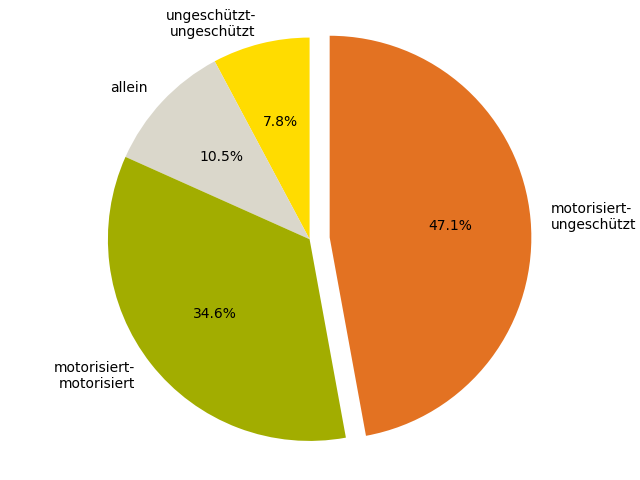
\includegraphics[width=8cm,height=6cm]{figures/motorisiert_ungeschuetzt}
		\caption[Beteiligung von motorisierten und ungeschützten Verkehrsteilnehmern an Unfällen mit Personenschaden, die in den Jahren 2012 bis 2016 im Testgebiet aufgenommen wurden]{Beteiligung von motorisierten und ungeschützten Verkehrsteilnehmern an Unfällen mit Personenschaden, die in den Jahren 2012 bis 2016 im Testgebiet aufgenommen wurden}\label{fig:Verkehrsbeteiligung_Personenschaden}
	\end{figure}
\end{savenotes}

In Abbildung \ref{fig:Verletzungsschwere_Pkw} ist die Verletzungsschwere von Pkw-Fahrern dargestellt. Andere motorisierte Verkehrsteilnehmer werden nicht betrachtet, da sie selten an Unfällen beteiligt sind (vgl. Abbildung \ref{fig:Beteiligungsart}). Pkws sind zwar häufig an Unfällen mit Personenschaden beteiligt, tragen aber selbst selten eine Verletzung davon. Lediglich in 10 \% der Unfälle mit Personenschaden wurde ein Pkw-Fahrer leicht verletzt.

\begin{savenotes}
	\begin{figure}[H]
		\centering
		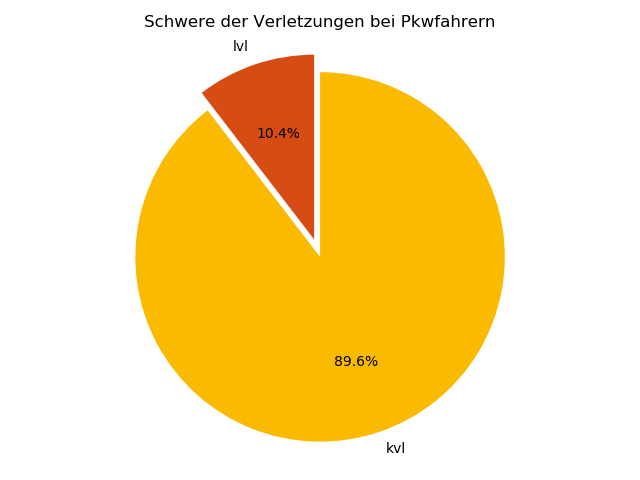
\includegraphics[width=8cm,height=6cm]{figures/Verl_Pkw}
		\caption[Schwere der Verletzungen von Pkw-Fahrern bei Unfällen mit Personenschaden, die in den Jahren 2012 bis 2016 im Testgebiet aufgenommen wurden ]{Schwere der Verletzungen von Pkw-Fahrern bei Unfällen mit Personenschaden, die in den Jahren 2012 bis 2016 im Testgebiet aufgenommen wurden}\label{fig:Verletzungsschwere_Pkw}
	\end{figure}
\end{savenotes}

Bei Radfahrern kommt es dagegen bei Unfällen mit Personenschaden in über 80 \% der Fälle zu Verletzungen. In 10 \% wurden Radfahrer sogar schwer verletzt. Fußgänger sind zwar seltener an Unfällen beteiligt, tragen dafür bei einer Unfallbeteiligung fast immer eine Verletzung davon. Im Untersuchungsgebiet kam es bei 93 \% der Unfälle, an denen Fußgänger beteiligt waren, zu einem Personenschaden. 80 \% führten zu einer leichten Verletzung, bei ca. 7 \% wurden die Fußgänger schwer oder tödlich verletzt. Abbildung \ref{fig:Verletzungsschwere_Rad_Fuss} stellt die Verletzungsschwere von Radfahrern und Fußgängern bei Unfällen mit Personenschaden dar. Die Annahme in \textit{Hypothese 5}, dass der Verletzungsgrad bei ungeschützten Verkehrsteilnehmern höher ist kann somit bestätigt werden.

\begin{savenotes}
	\begin{figure} [H]
		\subfigure{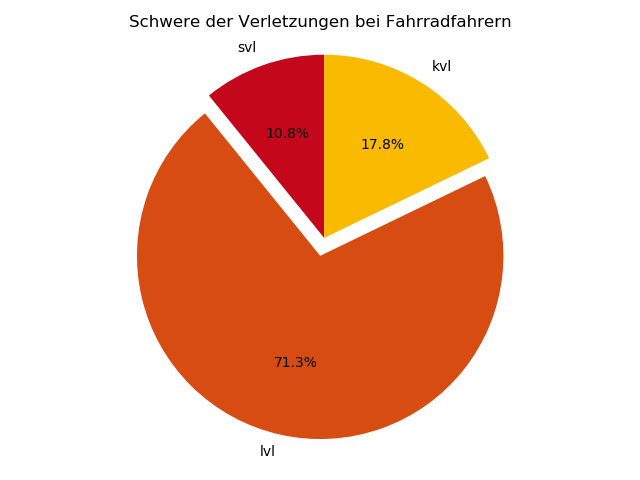
\includegraphics[width=0.49\textwidth,height=6cm]{figures/Verl_Rad}} 
		\subfigure{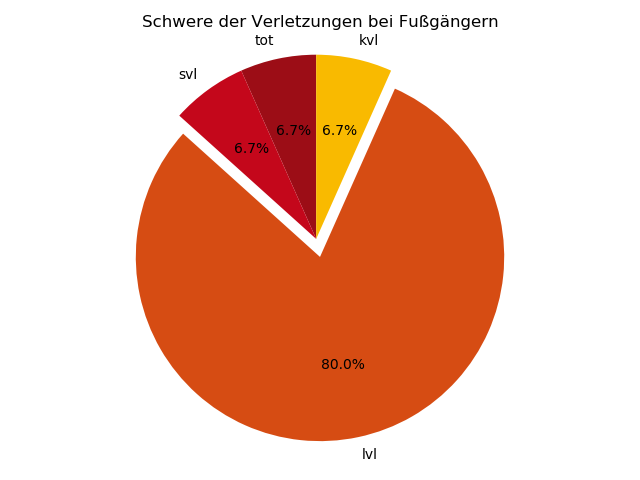
\includegraphics[width=0.49\textwidth,height=6cm]{figures/Verl_Fussg}} 
		\caption[Schwere der Verletzungen von Radfahrern und Fußgängern bei Unfällen mit Personenschaden, die in den Jahren 2012 bis 2016 im Testgebiet aufgenommen wurden ]{Schwere der Verletzungen von Radfahrern und Fußgängern bei Unfällen mit Personenschaden, die in den Jahren 2012 bis 2016 im Testgebiet aufgenommen wurden}\label{fig:Verletzungsschwere_Rad_Fuss} 
	\end{figure}
\end{savenotes}

\subsection{Unfälle mit Radfahrerbeteiligung beim Abbiegen}\label{subsection:Abbiegeunfälle mit Radfahrern}
Bei Unfällen, bei denen die Unfallursache \enquote{Fehler beim Abbiegen nach rechts} (34) angegeben wurde, kam es in 86 \% der Fälle zu Unfällen mit Radfahrern. Dabei waren die Radfahrer, bis auf eine Ausnahme, nicht Hauptverursacher des Unfalls. Bei den Hauptverursachern handelte es sich in fast 89 \% der Fälle um Pkw-Fahrer. Bei drei Unfällen waren Lkw-Fahrer die Hauptverursacher, bei jeweils einem Unfall ein Motorrad- und ein Reisebusfahrer. Insgesamt kam es innerhalb des Testgebiets im Untersuchungszeitraum zu 45 Unfällen mit Radfahrerbeteiligung, bei denen die Ursache \enquote{Fehler beim Abbiegen nach rechts} bei den jeweiligen Hauptverursachern des Unfalls angegeben wurde.

\begin{savenotes}
	\begin{figure}[H]
		\centering
		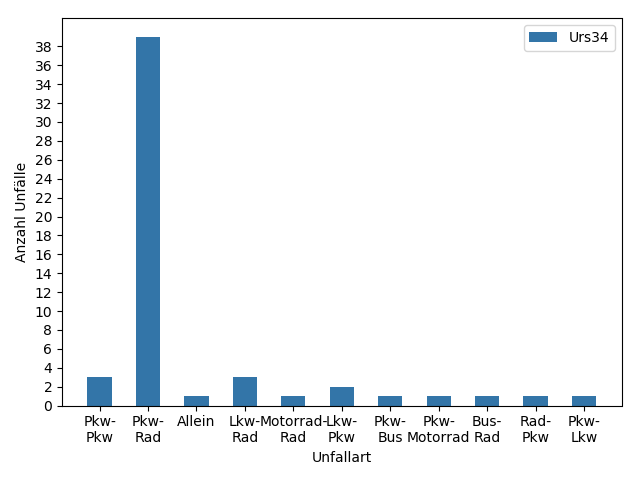
\includegraphics[width=8cm,height=6cm]{figures/Urs34_Beteiligung}
		\caption[Art der Verkehrsbeteiligung bei Unfällen mit der Unfallursache 34, die in den Jahren 2012 bis 2016 im Testgebiet aufgenommen wurden]{Art der Verkehrsbeteiligung bei Unfällen mit der Unfallursache 34, die in den Jahren 2012 bis 2016 im Testgebiet aufgenommen wurden}\label{fig:Urs34_Verkehrsbeteiligung}
	\end{figure}
\end{savenotes}

Die Ursache \enquote{Fehler beim Abbiegen nach links} (35) wurde lediglich bei ca. 26 \% der Unfälle mit Radfahrerbeteiligung angegeben. Hierbei war keiner der Radfahrer Hauptverursacher. Bei den Hauptverursachern handelte es sich bis auf einen Fall immer um Pkw-Fahrer. Innerhalb des Testgebiets ereigneten sich zwölf Unfälle mit Radfahrerbeteiligung, bei denen die Unfallursache 35 beim Hauptverursacher angegeben wurde. Die Abbildungen  zeigen, bei wie vielen Unfällen im Testgebiet die zwei genannten Ursachen mit den jeweiligen Unfallbeteiligten angegeben wurden. Auffällig ist, dass keine der beiden Ursachen bei Unfällen mit Fußgängern angegeben wurde, diese sind deshalb in den Abbildungen \ref{fig:Urs34_Verkehrsbeteiligung} und \ref{fig:Urs35_Verkehrsbeteiligung} nicht eingetragen.

\begin{savenotes}
	\begin{figure}[H]
		\centering
		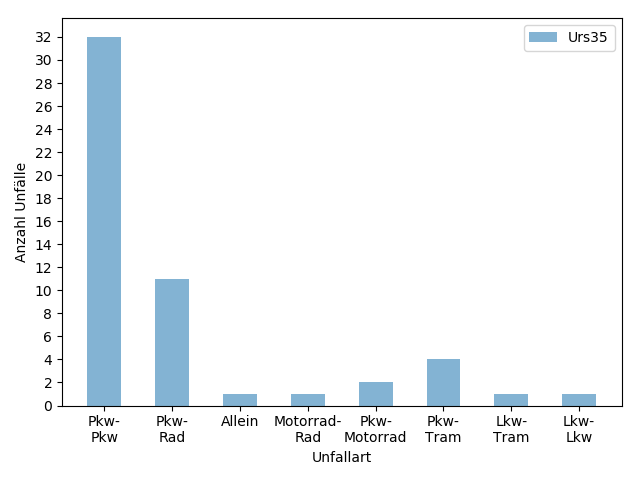
\includegraphics[width=8cm,height=6cm]{figures/Urs35_Beteiligung}
		\caption[Art der Verkehrsbeteiligung bei Unfällen mit der Unfallursache 35, die in den Jahren 2012 bis 2016 im Testgebiet aufgenommen wurden]{Art der Verkehrsbeteiligung bei Unfällen mit der Unfallursache 35, die in den Jahren 2012 bis 2016 im Testgebiet aufgenommen wurden}\label{fig:Urs35_Verkehrsbeteiligung}
	\end{figure}
\end{savenotes}

Betrachtet man die Unfallart, wurde bei den Unfällen mit der Ursache 34 und Radfahrerbeteiligung am häufigsten die Unfallart \enquote{Zusammenstoß mit Fahrzeug, das einbiegt oder kreuzt} genannt (5). Gefolgt von \enquote{Zusammenstoß mit Fahrzeug, das seitlich oder in gleiche Richtung fährt} (3) und \enquote{Zusammenstoß mit Fahrzeug, das entgegenkommt} (4). In einem Fall wurde die Ursache \enquote{Zusammenstoß mit Fahrzeug, das anfährt, anhält, im ruh. Verkehr steht} (1) genannt. Wie in Abbildung \ref{fig:Unfallart_Urs34_Urs35_Radbeteiligung} zu erkennen ist, weisen die Unfälle mit der Unfallursache 35 ein ähnliches Bild auf. Hier steht lediglich die Unfallart 4 an zweiter und die Unfallart 3 an dritter Position .

\begin{savenotes}
	\begin{figure}[H]
		\centering
		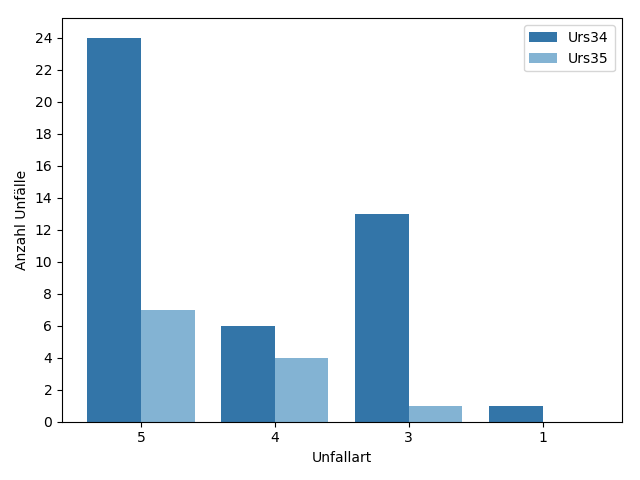
\includegraphics[width=8cm,height=6cm]{figures/Art_Urs34_Urs35}
		\caption[Unfallart bei Unfällen mit Radfahrerbeteiligung und Angabe der Unfallursache 34 bzw. 35, die in den Jahren 2012 bis 2016 im Testgebiet aufgenommen wurden]{Unfallart bei Unfällen mit Radfahrerbeteiligung und Angabe der Unfallursache 34 bzw. 35, die in den Jahren 2012 bis 2016 im Testgebiet aufgenommen wurden}\label{fig:Unfallart_Urs34_Urs35_Radbeteiligung}
	\end{figure}
\end{savenotes}

\textit{Hypothese 6} gibt an, dass sich beim Rechtsabbiegen häufiger Unfälle mit Radfahrern oder Fußgängern, die sich parallel zum Fahrzeug bewegen, ereignen als beim Linksabbiegen. Während sich deutlich mehr Unfälle mit Fahrradbeteiligung beim Rechtsabbiegen ereignen, kann zu Unfällen mit Fußgängerbeteiligung anhand der vorhandenen Daten keine Angabe gemacht werden. Ob sich die Radfahrer bei den Unfällen parallel zum Unfallverursacher bewegt haben, soll anhand der Unfallart überprüft werden. Wurde die Unfallart 3 oder 4 genannt, bewegten sich die Radfahrer parallel zum Unfallverursacher. Wurde die Unfallart 5 angegeben, ist zunächst davon auszugehen, dass sich die Radfahrer hier nicht parallel zum Fahrzeugverkehr bewegten. Bei einer stichprobenhaften Überprüfung der Kurzbeschreibungen für das Jahr 2013 bis 2016, ist zu erkennen, dass sich die Radfahrer auch hier häufig parallel zum Unfallverursacher bewegten. Da die Kurzbeschreibungen nicht für den gesamten Untersuchungszeitraum vorliegen, soll hier zunächst nur darauf hingewiesen werden, dass auch Unfälle der Art 5 mit parallelen Bewegungen stattfinden können. Insgesamt wurde die Unfallart 5, wie in Abbildung \ref{fig:Unfallart_Urs34_Urs35_Radbeteiligung} zu erkennen ist, häufiger angegeben als Unfallart 3 und 4 zusammen. Die Annahme in \textit{Hypothese 6}, dass sich die Unfallbeteiligten parallel bewegten, kann zunächst nicht bestätigt werden. Es sollte allerdings immer anhand der Kurzbeschreibungen überprüft werden, ob nicht auch Unfälle, bei denen die Unfallart 5 genannt wurde, solch ein Bewegungsmuster aufweisen.

Zusätzlich gibt \textit{Hypothese 6} an, dass kritische Situationen, vor allem dann entstehen, wenn Radfahrer den Radweg in die falsche Richtung befahren. Hierfür werden Unfälle mit Radfahrern im Untersuchungsgebiet betrachtet, bei denen die Ursachen \enquote{Verbotswidrige Benutzung der Fahrbahn oder anderer Straßenteile (z.B. Gehweg, Radweg)} (10) oder \enquote{Benutzung der Fahrbahn entgegen der vorgeschriebenen Fahrtrichtung in anderen Fällen} (9) angegeben wurden. Im Untersuchungszeitraum wurde bei insgesamt zwölf Unfällen mit Radfahrerbeteiligung die Ursache 10 angegeben. Mit einer Ausnahme wurde sie immer dem beteiligten Radfahrer zugeordnet. Es kam siebenmal zu Unfällen mit Pkw-Rad Beteiligung, viermal ereignete sich ein Unfall mit zwei Radfahrern und einmal kam es zu einem Unfall mit Rad-Pkw Beteiligung. Der Erstgenannte ist hierbei immer der Unfallverursacher. Die Unfallursache 9 wurde lediglich bei zwei Unfällen mit Radfahrerbeteiligung angegeben. Um diesen Teil der \textit{Hypothese 6} bestätigen zu können, müsste zu den Ursachen 10 und 9 noch die Ursachen 34 oder 35 angegeben werden. Es kommt im Untersuchungsgebiet jedoch nur zu einem Unfall mit Radbeteiligung, bei dem sowohl die Ursache 10 als auch die Ursache 35 aufgenommen wurden. \textit{Hypothese 6} kann daher in diesem Punkt nicht bestätigt werden.

\begin{savenotes}
	\begin{figure}[H]
		\centering
		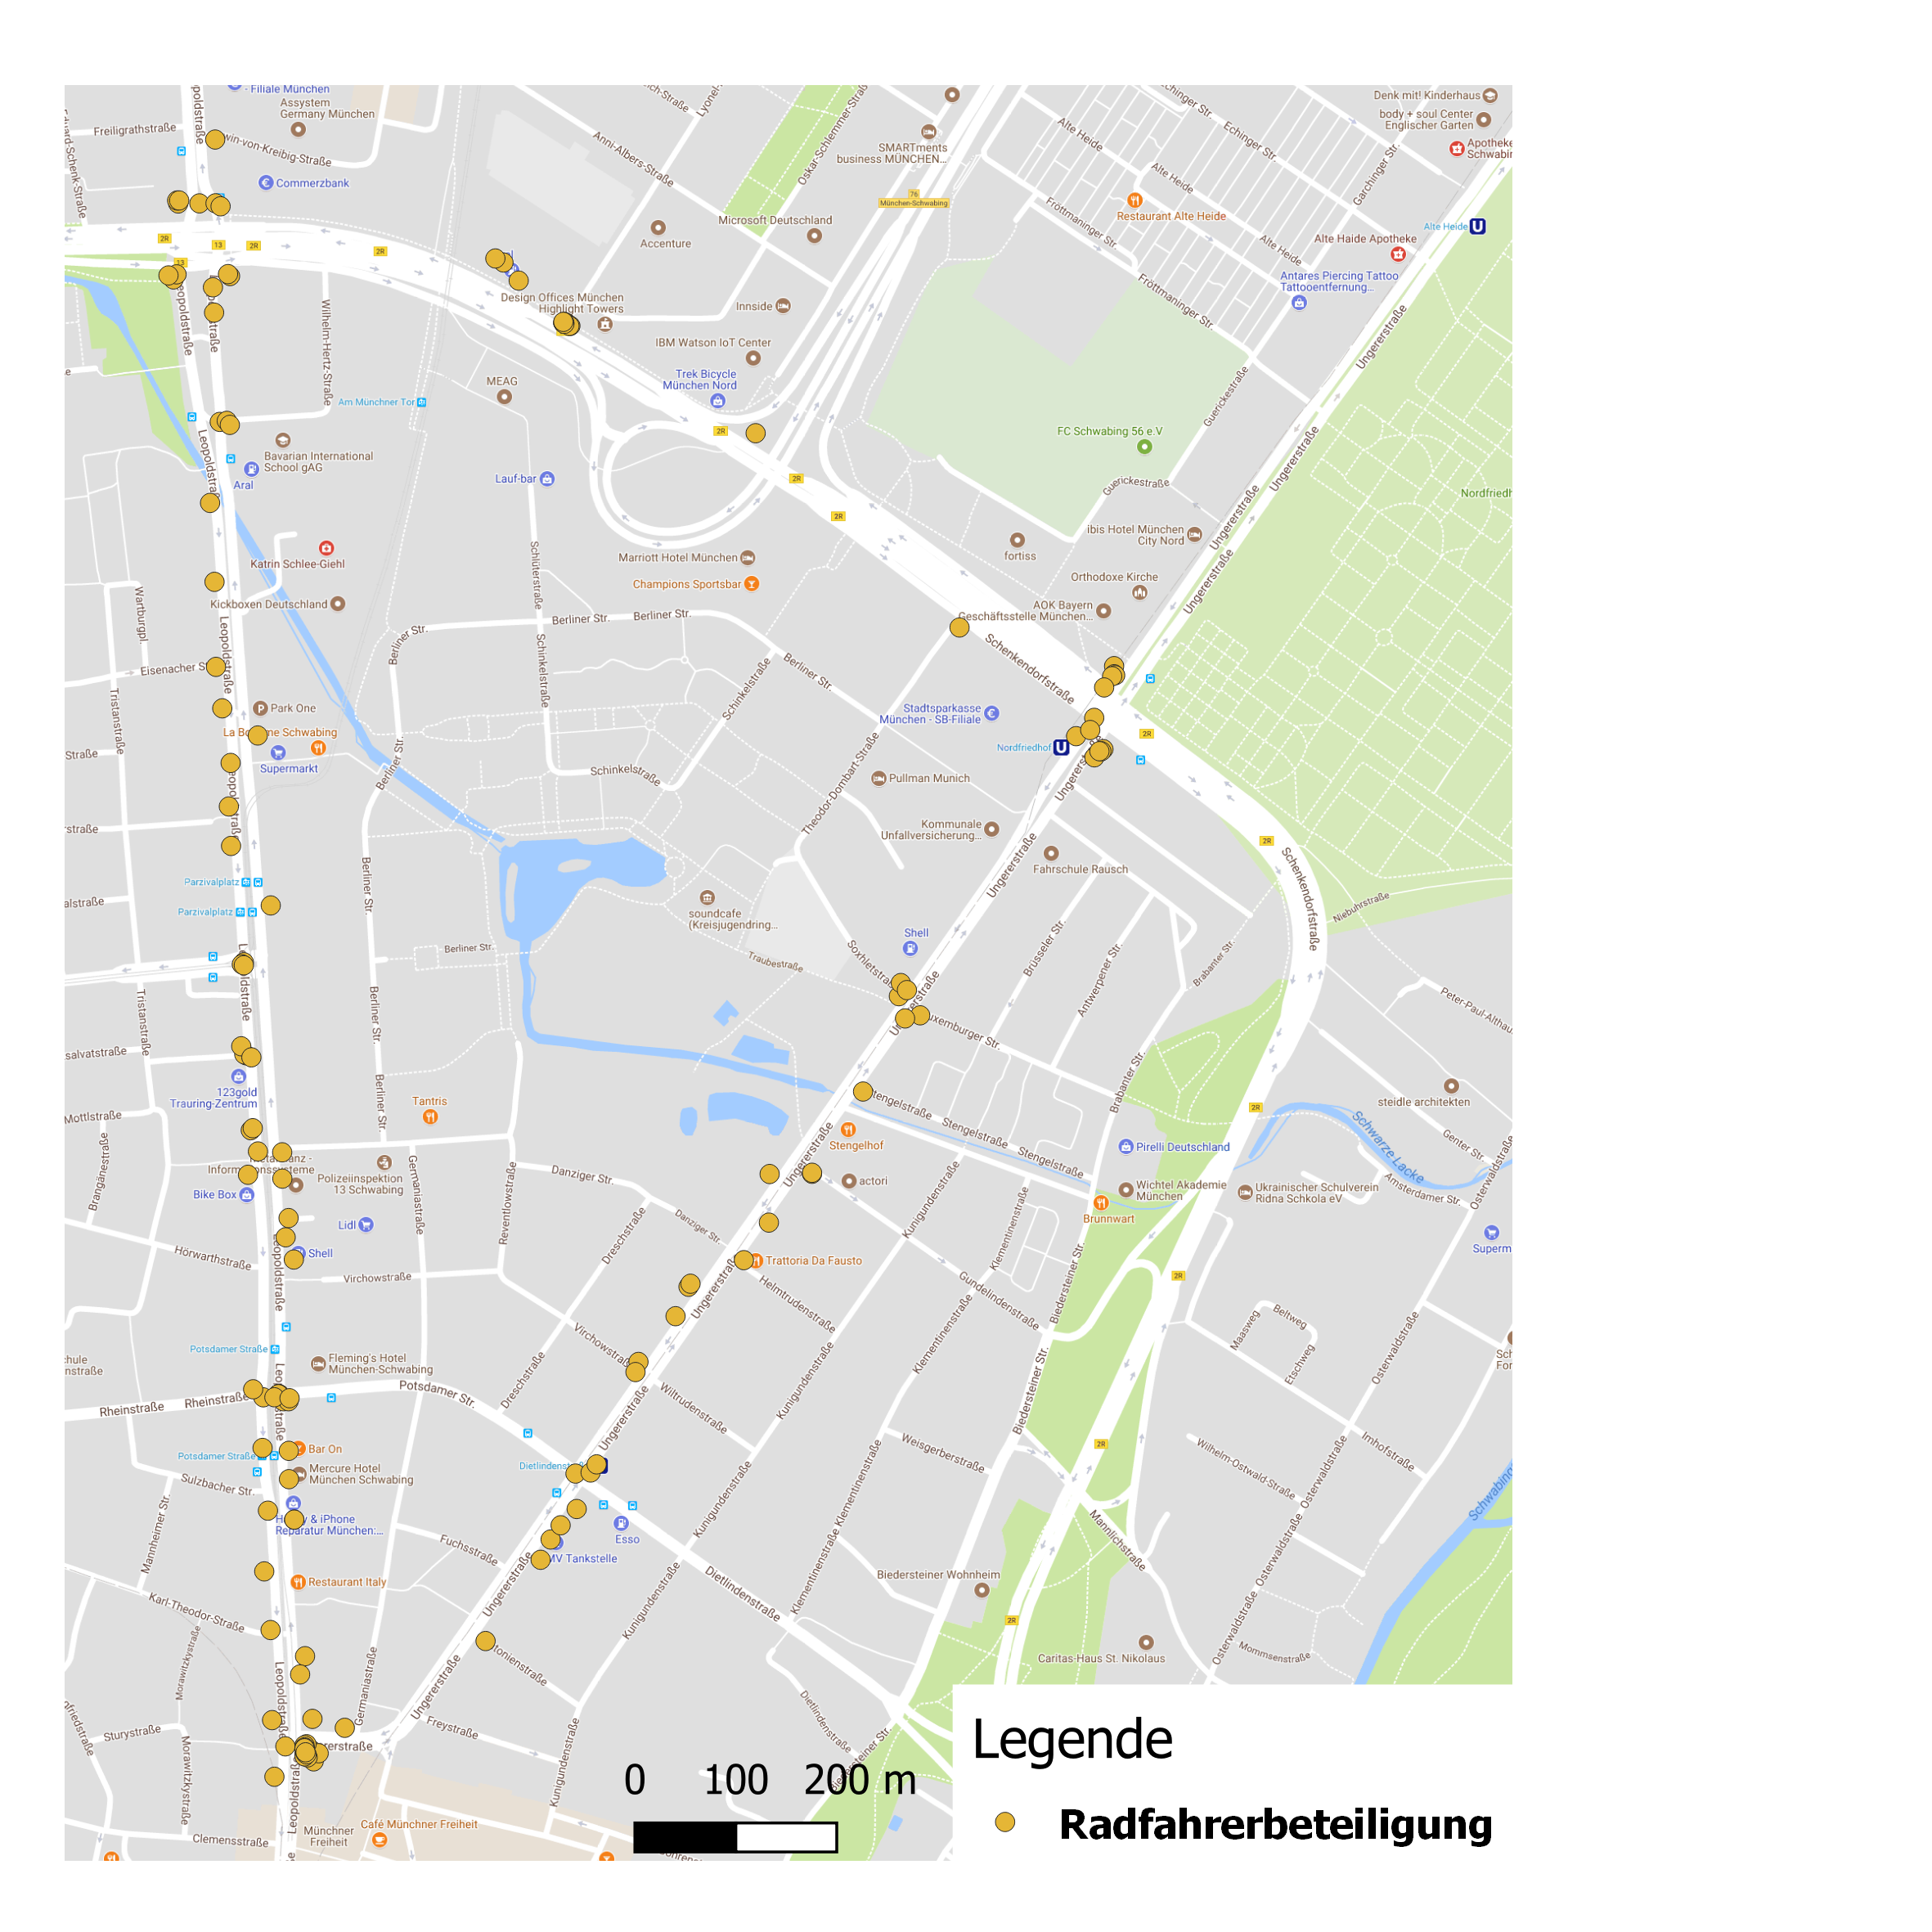
\includegraphics[width=10cm,height=10cm]{figures/map_radfahrer}
		\caption[Unfälle mit Fahrradbeteiligung, die in den Jahren 2012 bis 2016 im Testgebiet aufgenommen wurden]{Unfälle mit Fahrradbeteiligung, die in den Jahren 2012 bis 2016 im Testgebiet aufgenommen wurden}\label{fig:map_radfahrer}
	\end{figure}
\end{savenotes}

In Abbildung \ref{fig:map_radfahrer} werden die Unfälle mit Fahrradbeteiligung dargestellt. Hier ist zu erkennen, dass es an der Einmündung Leopoldstraße/Ungererstraße vermehrt zu Unfällen mit Fahrradfahrern kommt. Hierbei wurden 16 von 23 Unfällen durch Fehler beim Rechtsabbiegen ausgelöst. Es kommt vor allem zu Konflikten, wenn Fahrzeuge die Leopoldstraße in nördliche Richtung befahren und nach rechts auf die Ungererstraße abbiegen. Der Radweg darf hier in beide Richtungen befahren werden und ist im Bereich der Einmündung, zumindest im Konfliktbereich, rot eingefärbt. Abbildung \ref{fig:Konflikt_Ungerer_Leo} wurde mit Blick in Richtung Norden aufgenommen, die Einfärbung ist rechts im Bild gut zu erkennen. Laut Bildern von Google Earth wurde die Markierung im Jahr 2016 angebracht. Da die vorhanden Unfalldaten nur bis zum Jahr 2016 reichen, kann nicht geprüft werden, ob die Konflikte reduziert werden konnten.

%Bei Gelegenheit noch ein besseres Bild machen!!
\begin{savenotes}
	\begin{figure}[H]
		\centering
		\includegraphics[width=8cm,height=6cm]{figures/Ungerer_Leo}
		\caption[Konfliktpunkt an der Einmündung Leopoldstraße-Ungererstraße mit eingefärbter Radverkehrsanlage]{Konfliktpunkt an der Einmündung Leopoldstraße-Ungererstraße mit eingefärbter Radverkehrsanlage (aufgenommen am 20.08.2018)}\label{fig:Konflikt_Ungerer_Leo}
	\end{figure}
\end{savenotes}

\subsection{Fehlverhalten der Fußgänger}
Um Fehler von Fahrzeugführern und Fußgängern unterscheiden zu können, gibt es Unfallursachen, die das falsche Verhalten der Fußgänger beschreiben. In Abbildung \ref{fig:Fehlverhalten_Fussgaenger} ist zu erkennen, dass im Testgebiet die Ursache \enquote{ohne auf den Fzg.-verkehr zu achten} (64) am häufigsten angegeben wurde. Hierbei kam es fast immer zu einem Unfall mit Personenschaden.

An zweiter Position steht die Ursache \enquote{andere Fehler der Fußgänger} (69). Obwohl es bei sechs Unfällen einen Personenschaden gab, wurden keine weiteren Angaben gemacht, um welche Fehler es sich genau handelt. Während es sich bei der erst genannten Unfallursache meist um Situationen handelt, in denen Fußgänger einfach auf die Straße treten ohne den Fzg.-Verkehr zu beachten, kann dieser Punkt keiner bestimmten Situation im Straßenraum zugeordnet werden. Weitere Unfälle ereigneten sich \enquote{durch plötzliches Hervortreten hinter Sichthindernissen} (63), \enquote{in der Nähe von Kreuzungen oder Einmündungen, Lichtzeichenanlagen oder Fußgängerüberwegen, bei dichtem Verkehr an anderen Stellen} (62) oder durch \enquote{Nichtbenutzen des Gehwegs} (65). Wenn diese drei Unfallursachen angegeben wurden, kam es in acht von zehn Fällen zu einem Personenschaden. Etwas seltener und mit geringeren Folgen wurden dagegen die Ursachen \enquote{Nichtbenutzen der vorgeschrieben Straßenseite} (67) und \enquote{Nichtbenutzen des Gehwegs} (66) angegeben.

\begin{savenotes}
	\begin{figure}[H]
		\centering
		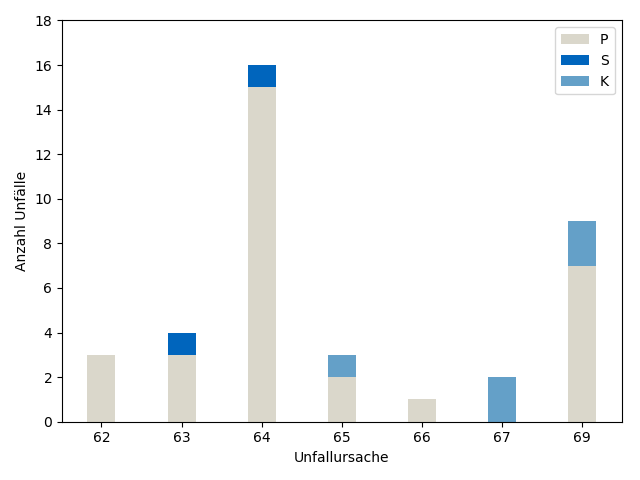
\includegraphics[width=8cm,height=6cm]{figures/Urs_Fussgaenger}
		\caption[Unfallursachen durch falsches Verhalten der Fußgänger mit zugehörigem Unfallmodus, die bei Unfällen in den Jahren 2012 bis 2016 im Testgebiet angegeben wurden]{Unfallursachen durch falsches Verhalten der Fußgänger mit zugehörigem Unfallmodus, die bei Unfällen in den Jahren 2012 bis 2016 im Testgebiet angegeben wurden}\label{fig:Fehlverhalten_Fussgaenger}
	\end{figure}
\end{savenotes}

In Abbildung \ref{fig:Beteiligungsart} ist zu erkennen, dass bei etwas mehr als der Hälfte der Unfälle mit Fußgängerbeteiligung, Fußgänger selbst die Hauptverursacher sind. Betrachtet man hier nochmals die Unfallursache \enquote{ohne auf den Fzg.-verkehr zu achten}, wurden sogar bei ca. 81 \% der Unfälle Fußgänger als Hauptbeteiligter angegeben.

\textit{Hypothese 8} gibt an, dass falsches Verhalten der Fußgänger häufig die Ursache für Unfälle mit Personenschaden im urbanen Raum ist. Im Vergleich zu Kfz sind Fußgänger zwar seltener an Unfällen beteiligt, dafür kommt es bei einer Beteiligung häufig zu Personenschaden. Im Testgebiet gab es innerhalb von fünf Jahren 36 Unfälle mit Fußgängerbeteiligung, dabei kam es bei 30 zu einem Personenschaden. Betrachtet man alle Unfälle mit Personenschaden im Untersuchungsgebiet, wurde immerhin bei 10 \% der Unfälle als Unfallursache falsches Verhalten der Fußgänger angegeben. \textit{Hypothese 8} kann daher in diesem Punkt bestätigt werden.

Zusätzlich wurde in \textit{Hypothese 8} angenommen, dass die Unfallursachen Rotlichtverstöße (60) und \enquote{Überschreiten der Fahrbahn ohne auf den Fzg.-verkehr zu achten} dabei am häufigsten vorkommen. In Abbildung \ref{fig:Fehlverhalten_Fussgaenger} ist zu erkennen, dass Rotlichtverstöße innerhalb von fünf Jahren im Untersuchungsgebiet gar nicht aufgenommen wurden, während \enquote{Überschreiten der Fahrbahn ohne auf den Fzg.-verkehr zu achten} am häufigsten genannt wurde. Abbildung \ref{fig:Verletzungen_Urs64} bezieht sich nur auf diese Ursache und gibt die Schwere der Verletzungen an. Hierbei ist auffällig, dass lediglich bei 12,5 \% der am Unfall Beteiligten \ac{kvl} vorlag. Bei über 60 \% kam es zu leichten Verletzungen (lvl) und in jeweils 12,5 \% der Fälle wurden Unfallbeteiligte schwer (svl) oder sogar tödlich verletzt (tot). Eine tödliche Verletzung trat im gesamten Untersuchungsgebiet innerhalb des Untersuchungszeitraums nur bei zwei Unfällen auf, diese machen genau die eben genannten 12,5 \% der Unfallursache 64 aus. \textit{Hypothese 8} kann im zweiten Teil nur in einem Punkt bestätigt werden, der dafür einen wesentlichen Einfluss auf Unfälle mit Personenschaden hat.

\begin{savenotes}
	\begin{figure}[H]
		\centering
		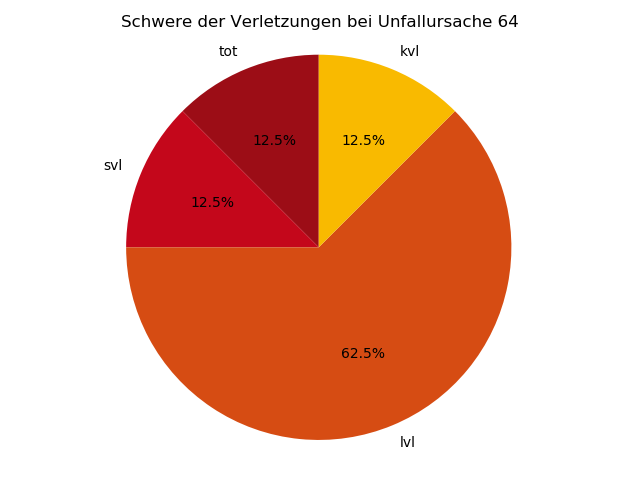
\includegraphics[width=8cm,height=6cm]{figures/Urs64}
		\caption[Verletzungen, die durch Unfälle mit Angabe der Ursache 64 bei Unfällen in den Jahren 2012 bis 2016 im Testgebiet angegeben wurden]{Verletzungen, die durch Unfälle mit Angabe der Ursache 64 bei Unfällen in den Jahren 2012 bis 2016 im Testgebiet angegeben wurdenn}\label{fig:Verletzungen_Urs64}
	\end{figure}
\end{savenotes}


Betrachtetet man die den Unfällen mit Fußgängerbeteiligung zugeordneten Besonderheiten wurden im Testgebiet nur vier Mal \enquote{Fußgängerfurt} und sechs Mal \enquote{Haltestelle} angegeben. Überraschend ist, dass es bei \enquote{Fußgängerüberwegen} keinen Unfall mit Fußgängern gab, obwohl diese Besonderheit in Abbildung \ref{fig:BES} am häufigsten vorkommt. In \textit{Hypothese 8} wird vermutet, dass sich Unfälle mit Fußgängern häufig in der Nähe von ÖPNV Haltestellen ereignen.

\begin{savenotes}
	\begin{figure}[H]
		\centering
		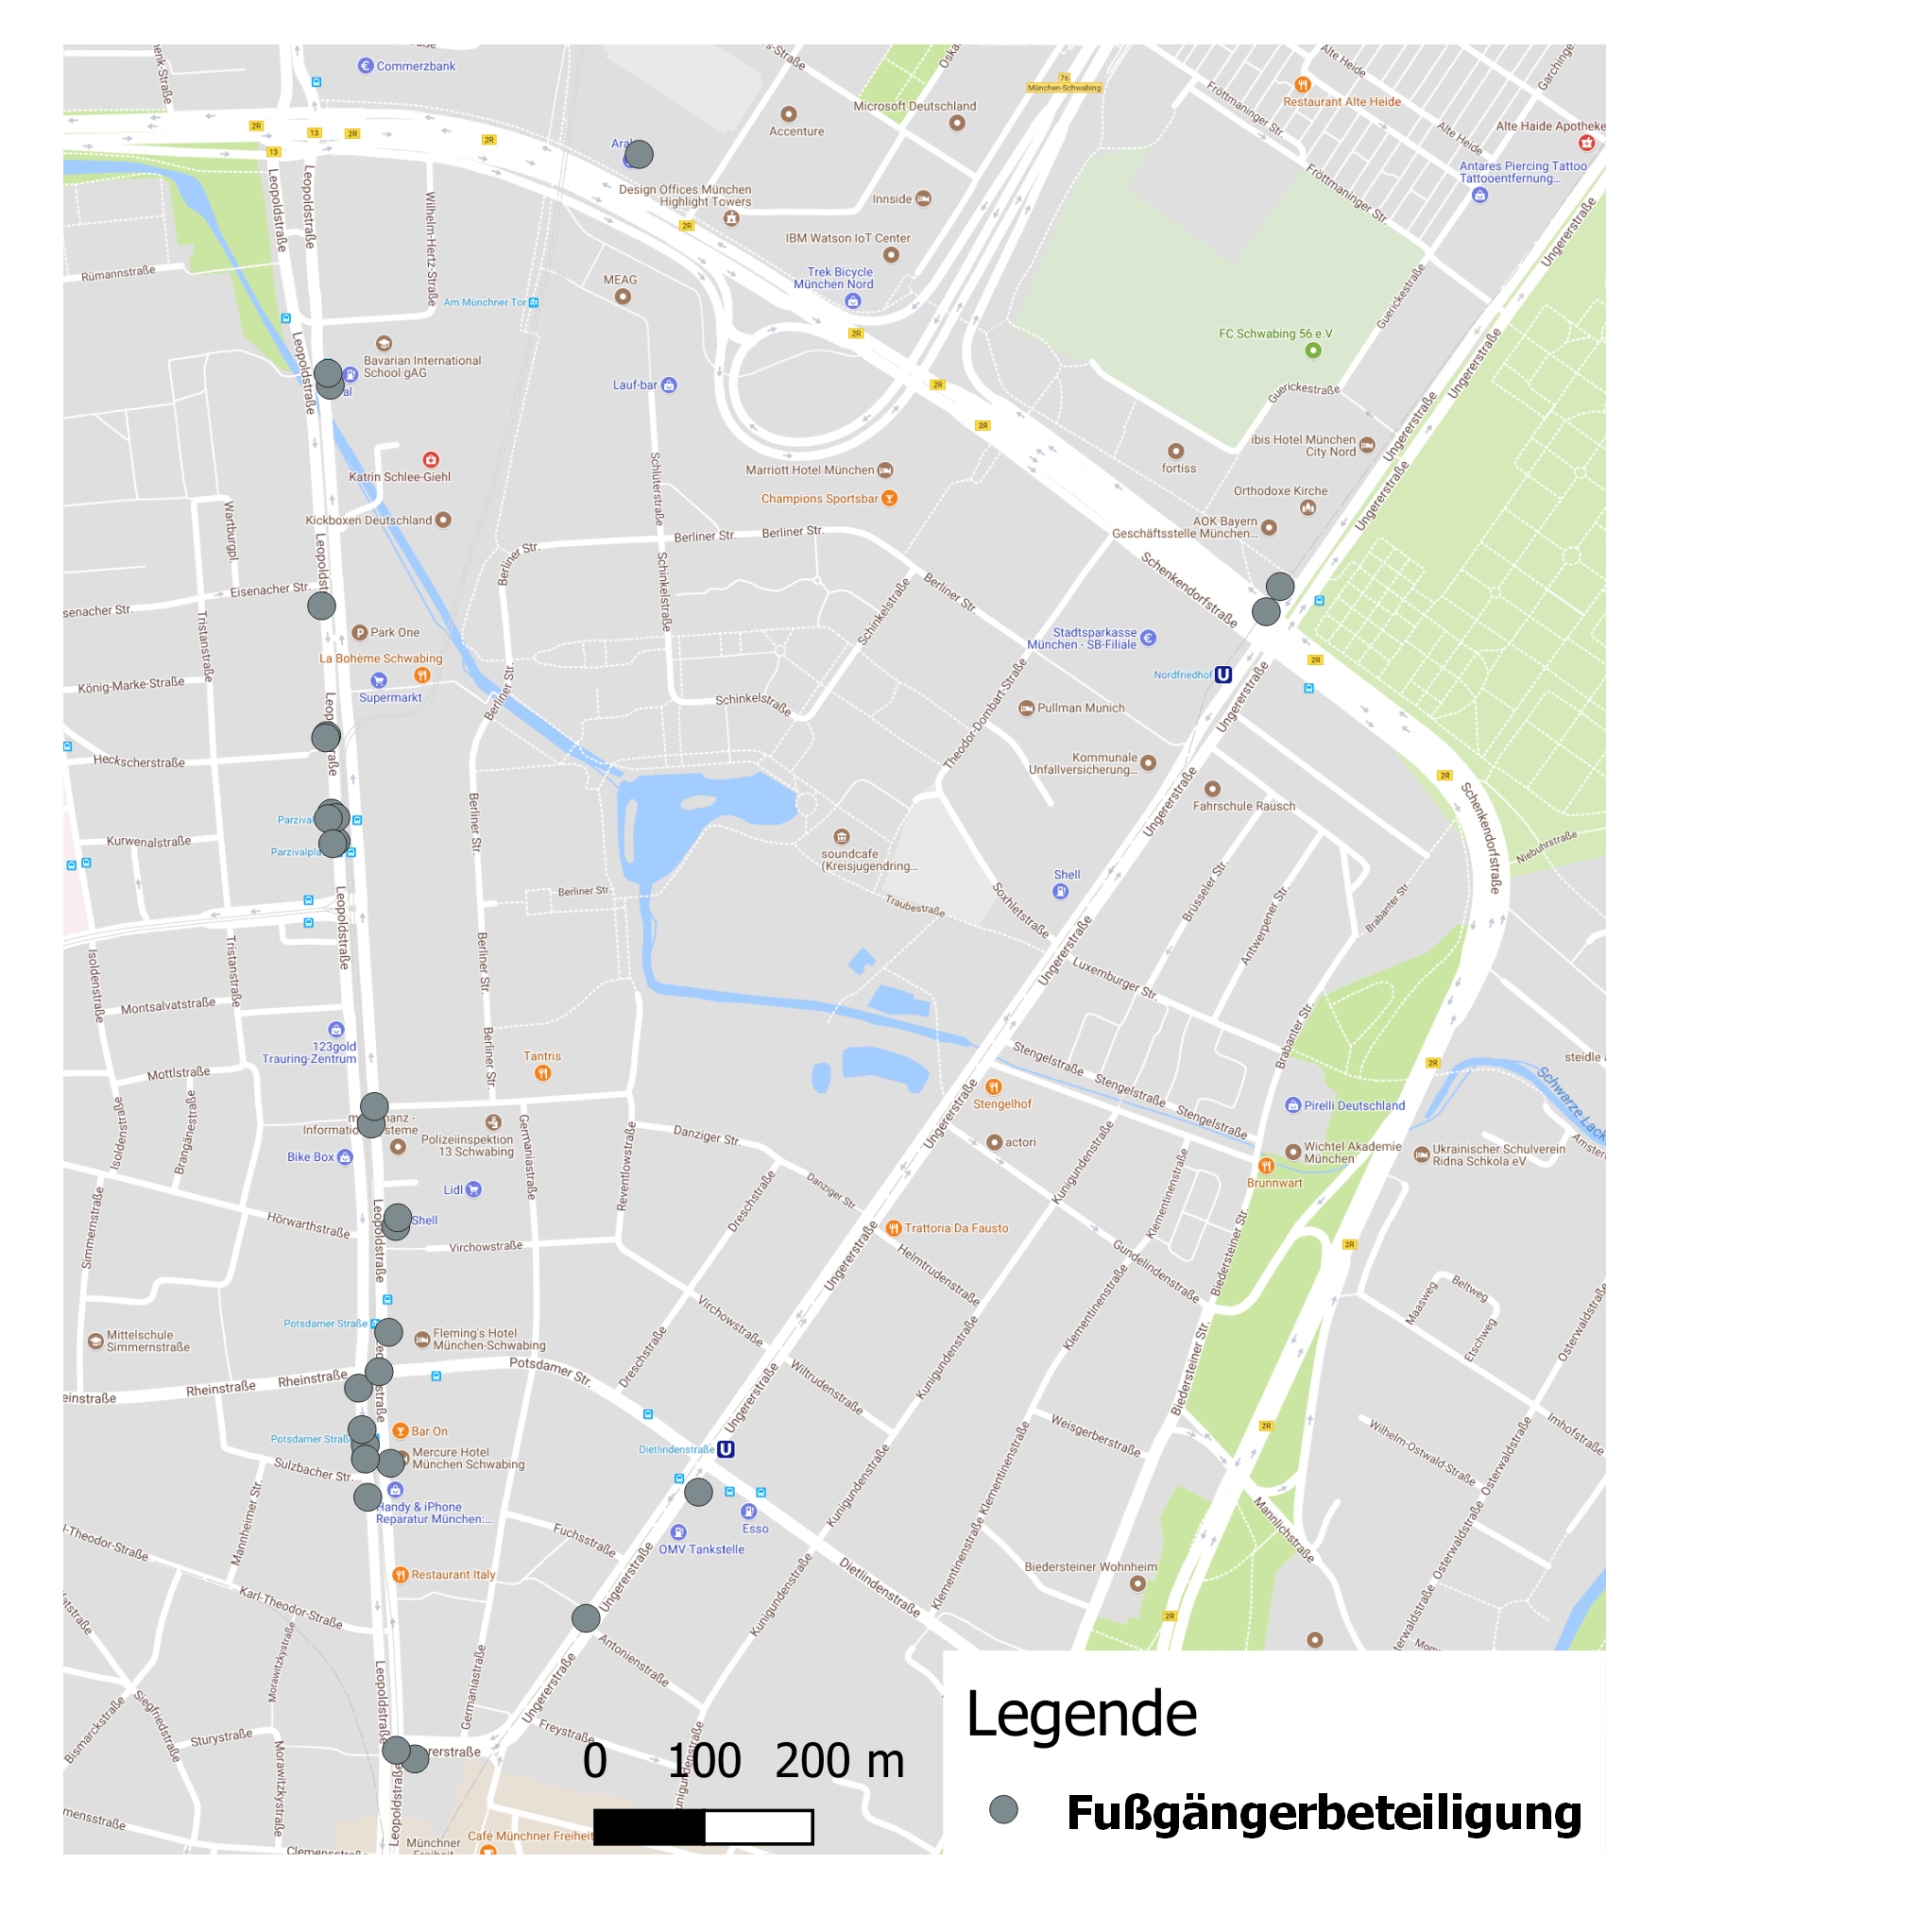
\includegraphics[width=10cm,height=10cm]{figures/map_fussgaenger}
		\caption[Unfälle mit Fußgängerbeteiligung, die in den Jahren 2012 bis 2016 im Testgebiet aufgenommen wurden]{Unfälle mit Fußgängerbeteiligung, die in den Jahren 2012 bis 2016 im Testgebiet aufgenommen wurden}\label{fig:map_fussganeger}
	\end{figure}
\end{savenotes}

In Abbildung \ref{fig:map_fussganeger} ist zu erkennen, dass sich vor allem im Bereich der Haltestellen Parzivalplatz und Potsdamer Straße Unfälle ereigneten. Am Parzivalplatz ereigneten sich fast 17 \% der Unfälle mit Fußgängerbeteiligung, im Bereich der Haltestelle Potsdamer Straße sogar 23 \%. Die beiden tödlichen Unfälle im Untersuchungszeitraum traten jeweils an einer der Haltestellen auf. \textit{Hypothese 8} kann somit in diesem Punkt bestätigt werden. Auffällig ist auch, dass bis auf fünf, alle Unfälle, bei denen Fußgänger beteiligt waren auf der Leopoldstraße aufgenommen wurden.

\subsection{Besonderheiten der Unfallstelle}
Besonderheiten der Unfallstelle werden nur bei Unfällen mit Personen- und Sachschaden angegeben. Innerhalb des Testgebiets wurden in fünf Jahren bei 11,9 \% der Unfälle mit Personenschaden und bei lediglich 3,7 \% mit Sachschaden Besonderheiten angegeben. In Abbildung \ref{fig:BES} werden die angegebenen Besonderheiten mit zugehörigem Unfallmodus dargestellt. Am häufigsten wurde als Besonderheit \enquote{Fußgängerüberweg} (3) angegeben. Gefolgt von \enquote{Fußgängerfurt} (4) und \enquote{Haltestelle} (5). Betrachtet man diese drei Punkte genauer, fällt auf, dass es bei Unfällen, an denen die Besonderheit \enquote{Haltestelle} genannt wurde, am häufigsten zu Unfällen mit Personenschaden kam. Unfälle an Fußgängerfurten führen ebenfalls häufiger zu Personen- als zu Sachschaden, während bei Fußgängerüberwegen die Unfälle mit Sachschaden überwiegen. Neben Fußgängerüberweg gibt es noch den \enquote{Schienengleichen Wegübergang} (2). Diese Besonderheit wurde im Untersuchungsgebiet nur in zwei Fällen angegeben. Hierbei muss darauf hingewiesen werden, dass diese Eigenschaft nur in der Leopoldstraße, in dem Bereich mit Tram, angegeben werden kann.

In lediglich einem Fall wurde \enquote{Unübersichtlich} (1) als Besonderheit angegeben und in drei Fällen war eine \enquote{Arbeitsstelle} (6) im Bereich des Unfallorts vorhanden. Da sich innerhalb der Teststrecke kein verkehrsberuhigter Bereich befindet, wurde diese Besonderheit (7) auch nie angegeben. 

\begin{savenotes}
	\begin{figure}[H]
		\centering
		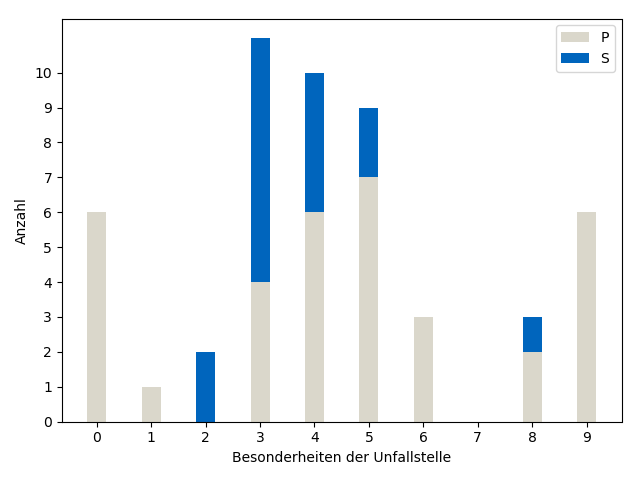
\includegraphics[width=8cm,height=6cm]{figures/BES}
		\caption[Besonderheiten der Unfallstelle mit zugehörigem Unfallmodus, die bei Unfällen in den Jahren 2012 bis 2016 im Testgebiet angegeben wurden]{Besonderheiten der Unfallstellen mit zugehörigem Unfallmodus, die bei Unfällen in den Jahren 2012 bis 2016 im Testgebiet angegeben wurden}\label{fig:BES}
	\end{figure}
\end{savenotes}

Bei Unfällen mit Personenschaden wurden die Besonderheiten \enquote{Benutzungspflicht der Radverkehrsanlage} (0) und \enquote{baulich von der Fahrbahn getrennte Radverkehrsanlage} am zweithäufigsten angegeben. Auffällig ist, dass diese Besonderheiten nur bei Unfällen mit Personenschaden angegeben wurden. \enquote{Radverkehrsanlagen auf der Fahrbahn oder lediglich durch Markierung von der Fahrbahn abgetrennt} (8) wurde im Vergleich zu den zwei vorherigen Besonderheiten seltener angegeben. Während die Besonderheiten 7 und 9 jeweils 2 \% der Unfälle mit Personenschaden ausmachen, wurde 8 nur in 0,8 \% der Fälle genannt.

\textit{Hypothese 7} gibt an, dass es bei baulich getrennten Radverkehrsanlagen häufiger zu Unfällen kommt als bei Radverkehrsanlagen auf der Fahrbahn. Die Anzahl der Unfälle, bei denen diese zwei Punkte als Besonderheit genannt wurden ist zwar gering, trotzdem ist in Abbildung \ref{fig:BES} zu erkennen, dass es bei baulich getrennten Radverkehrsanlagen häufiger zu Unfällen  kam. Hierbei muss jedoch beachtet werden, dass innerhalb des Testgebiets größtenteils nur derartige Radverkehrsanlagen vorhanden sind. Betrachtet man diese zwei Besonderheiten etwas genauer, fällt auf, dass die Radfahrer ungefähr zu gleichen Teilen als Beteiligter01 und Beteiligter02 angegeben werden. Zudem kommt es auf baulich getrennten Radverkehrsanlagen häufig zu Unfällen zwischen zwei Radfahrern oder zwischen Fahrrad und Fußgänger bzw. Fahrrad und Moped. Die Unfälle, bei denen angegeben wurde, dass es sich um Radverkehrsanlagen auf der Fahrbahn handelt, wiesen alle einen Konflikt zwischen Pkw und Fahrrad auf.

Im Testgebiet traten an der Einmündung Schenkendorfstraße/Leyonel-Feininger-Straße häufig Unfälle mit Fahrradbeteiligung auf. Hierbei wurde bei zwei Unfällen die Besonderheit \enquote{Radverkehrsanlage auf der Straße} und bei einem \enquote{getrennte Radverkehrsanlage} angegeben. Bei den ersten zwei Unfällen ereignete sich der Unfall direkt am Knotenpunkt. Es kam dabei jeweils zu einem Unfall zwischen einem Pkw, der nach rechts auf die Schenkendorfstraße einbiegen wollte und einem Radfahrer, der von rechts kam. Der Radweg darf an dieser Stelle in beide Richtungen befahren werden. Der dritte Unfall trat an der Tankstelle unmittelbar neben der Einmündung auf. Auch hier wollte ein Pkw nach rechts einbiegen und übersah einen von rechts kommenden Radfahrer. Da dieser Unfall sich allerdings im Bereich der Tankstelle ereignete wurde getrennte Radverkehrsanlage als Besonderheit angegeben. Die beiden Stellen sind in Abbildung \ref{fig:Lyonel-Feininger} zu erkennen. In diesem Fall ist nicht die Art der Radverkehrsanlage für die Unfallhäufungen verantwortlich, sondern die Freigabe des Radwegs entgegen der Fahrtrichtung. Mit dieser Situation rechnen Fahrzeugführer häufig nicht, obwohl an der Einmündung, vgl. Abbildung \ref{fig:Lyonel-Feininger}, deutlich kenntlich gemacht wurde, dass Radfahrer von beiden Seiten kommen können. Die Markierungen waren laut Bildern von Google Earth auch schon zu den jeweiligen Unfallzeitpunkten vorhanden.

\begin{savenotes}
	\begin{figure}[H]
		\centering
		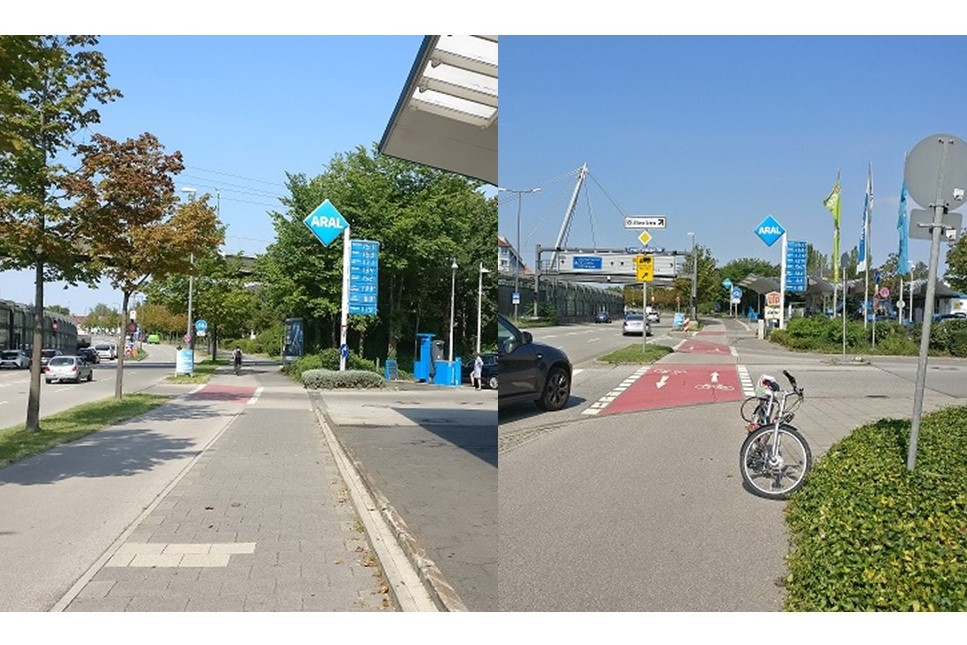
\includegraphics[width=12cm,height=8cm]{figures/Lyonel_Feininger}
		\caption[Ausfahrt Aral Tankstelle und Einmündung Lyonel-Feininger-Straße]{Links: Ausfahrt der Aral Tankstelle mit baulich von der Fahrbahn getrennter Radverkehrsanlage Rechts: Einmündung mit markiertem Radweg auf der Fahrbahn (aufgenommen am 20.08.2018)}\label{fig:Lyonel-Feininger}
	\end{figure}
\end{savenotes}

\textit{Hypothese 7} kann daher nur bedingt bestätigt werden. Sie wird zunächst anhand der statistischen Auswertung in Abbildung \ref{fig:BES} bekräftigt. Das Unfallgeschehen an der Einmündung Lyonel-Feininger-Straße macht dagegen deutlich, dass nicht nur die Art der Radverkehrsanlage sondern auch die Führung der Radfahrer von Bedeutung ist. Zusätzlich scheint der Einfluss der vorhandenen Markierung, trotz Roteinfärbung, nicht den gewünschten Effekt zu erbringen. Dies kann jedoch nicht nachgewiesen werden, da keine Unfallzahlen für einen Zeitraum vorliegen, in dem keine Markierung vorhanden war. 

%Statistischer Test um Aussagekraft zu belegen?

\subsection{Einfluss allgemeiner Unfallursachen}
Neben den persönlichen Ursachen können je Unfall bis zu zwei allgemeine Ursachen angegeben werden. Abbildung \ref{fig:allg_Ursachen} zeigt die allgemeinen Ursachen, die Unfällen im Testgebiet zugewiesen wurden. Es ist zu erkennen, dass \enquote{Glätte oder Schlüpfrigkeit der Fahrbahn} (70 bis 74) neben dem Punkt \enquote{Sonstige Ursachen} (89) am häufigsten zu Unfällen führten. Obwohl sonstige Ursachen am häufigsten genannt wurden, können sie hier nicht näher betrachtet werden, da keine zusätzlichen Beschreibungen über die Art vorliegen. Auffällig ist, dass \enquote{Schnee, Eis} (72) zwar häufiger als Unfallursache angegeben wurden, \enquote{Regen} (72) dafür zu mehr Unfällen mit Personenschaden führt. 

\begin{savenotes}
	\begin{figure}[H]
		\centering
		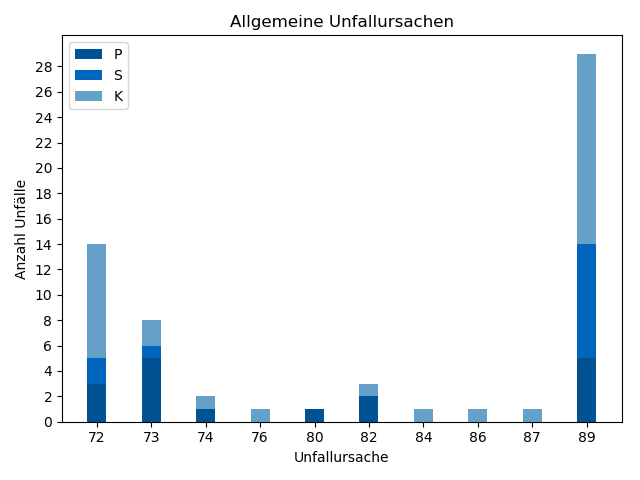
\includegraphics[width=8cm,height=6cm]{figures/allg_Ursachen}
		\caption[Allgemeine Unfallursachen mit Unfallmodus, die bei Unfällen in den Jahren 2012 bis 2016 im Testgebiet angegeben wurden]{Allgemeine Unfallursachen mit Unfallmodus, die bei Unfällen in den Jahren 2012 bis 2016 im Testgebiet angegeben wurden}\label{fig:allg_Ursachen}
	\end{figure}
\end{savenotes}

Witterungseinflüsse können nicht nur die Straßenverhältnisse beeinflussen sondern auch zu Sichtbehinderungen führen (Unfallursachen 80 bis 84). Innerhalb von fünf Jahren wurde im Testgebiet jedoch nur bei fünf Unfällen eine dieser Ursachen angegeben. Jeweils ein Unfall wurde durch \enquote{starken Regen, Hagel, Schnee} (81) bzw. \enquote{Unwetter} (84) und drei durch \enquote{blendende Sonne} (82) beeinflusst. Zwei der Unfälle, die sich durch Sonnenblendung ereigneten, hatten einen Personenschaden zur Folge. Betrachtete man jedoch alle Unfälle mit Personenschaden im Untersuchungsgebiet über die fünf Jahre, wurden lediglich 0,7 \% durch Sonnenblendung beeinflusst.

\textit{Hypothese 9} gibt an, dass es bei Sichtbehinderung durch blendende Sonne vermehrt zu Unfällen kommt. Blendende Sonne wird zwar im Vergleich zu den anderen Ursachen am häufigsten genannt, aber trotzdem zu selten, um ihr eine wirkliche Bedeutung zukommen zu lassen. \textit{Hypothese 9} kann daher nicht bestätigt werden. Trotzdem sollte man die Einwirkung durch blendende Sonne mit Fokus auf Kapitel \ref{chapter:automatisiertes Fahren} nicht vernachlässigen, Sensoren von automatisierten Fahrzeugen könnten hier Schwierigkeiten haben.
 
Noch seltener haben der \enquote{Zustand der Straße} (75 bis 79) und \enquote{Hindernisse} Einfluss auf Unfälle innerhalb des Testgebiets. Sie werden in Summe nur dreimal genannt und deshalb nicht näher betrachtet. Allgemeine Unfallursachen, die in dem betrachteten Zeitraum nie einem Unfall zugewiesen wurden, werden in Abbildung \ref{fig:allg_Ursachen} nicht berücksichtigt.

%Allg Fazit?

\section{Bewertung der Unfälle im Testgebiet}\label{section:Bewertung der Unfälle im Testgebiet}
Die Unfälle werden nun anhand der Bewertungsmethodik, die in Kapitel \ref{section:Bewertung urbaner Fahrsituationen} vorgestellt wird, bezüglich ihrer Kritikalität bewertet. Hierfür werden zunächst nur die Unfälle herangezogen, denen bei der Unfallaufnahme bereits ein Unfalltyp zugeordnet wurde. Anschließend werden alle Unfälle typisiert, um die Unfallabläufe besser verstehen zu können. Bei der Bewertung der typisierten Unfälle können so auch die Kleinunfälle berücksichtigt werden. Im Folgenden werden zuerst nur die sieben Unfalltypen betrachtet und dann die jeweiligen Feintypen.

\subsection{Bewertung der Unfälle mit zugeordnetem Unfalltyp}
Betrachtet man nur die Unfälle, denen bereits bei der Unfallaufnahme ein Unfalltyp zugeordnet wurde, werden die Kleinunfälle nicht berücksichtigt und die Gesamtanzahl der Unfälle beträgt lediglich 591 Stück. In Abbildung \ref{fig:Bewertung_UT} werden all diese Unfälle anhand des Unfalltyps, der Unfallschwere und der aufgetretenen Häufigkeit dargestellt. Es ist zu erkennen, dass zwei Unfalltypen ein erhöhtes Risiko aufweisen.

\begin{savenotes}
	\begin{figure}[H]
		\centering
		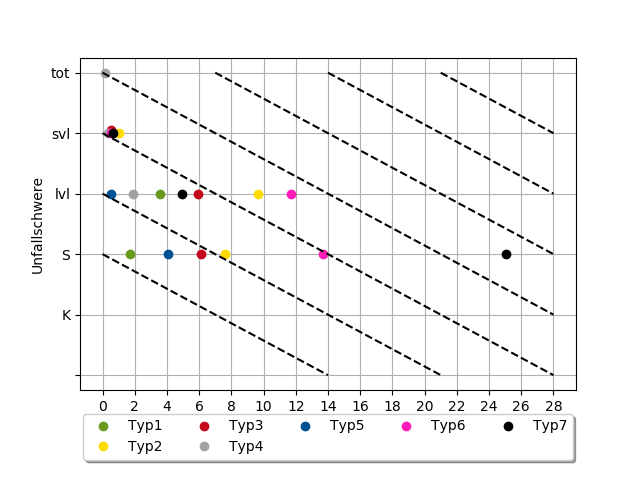
\includegraphics[width=12cm,height=8cm]{figures/Bewertung_UT}
		\caption[Bewertung anhand der während der Unfallaufnahme zugeordneten Unfalltypen]{Bewertung anhand der während der Unfallaufnahme zugeordneten Unfalltypen}\label{fig:Bewertung_UT}
	\end{figure}
\end{savenotes}

Die Typen 4 und 6 befinden sich in der Risiko-Kategorie \textit{d}. Auffällig ist, dass Typ 4 aufgrund der Unfallfolgen, im  betrachteten Zeitraum kam es nur bei Überschreit-Unfällen zu Getöteten, ein erhöhtes Risiko aufweist. Typ 7 dagegen wird wegen häufig aufgetretener Schachschadensunfälle der Kategorie \textit{d} zugeordnet. Bei ca. 25 \% der Unfälle im Untersuchungsgebiet wurde der Unfalltyp 7 in Kombination mit einem Sachschadensunfall angegeben.

Bei den Unfalltypen 1, 2, 3 und 6 kam es zu Unfällen mit Schwerverletzten. Schwere Verletzungen traten zwar pro Unfalltyp in weniger als 2 \% der Fälle auf, trotzdem reicht dies aus, um den Unfällen die Kategorie \textit{c} zuzuordnen. Bei den Typen 2 und 6 ist zudem auffällig, dass auch die Anzahl der Unfälle, bei denen es Leichtverletzte gab, mit ca. 9,5 \% (Typ 2) bzw. 11,5 \% (Typ 6) im selben Risikobereich angeordnet sind.

Der Typ 5, Unfälle im ruhenden Verkehr, bringt in diesem Fall das geringste Risiko mit sich. Es ereigneten sich hier nur wenig Unfälle mit Leichtverletzten. Zudem liegt die Anzahl der Unfälle mit Sachschaden nur bei 4 \%, weshalb diesem Typ die Risiko-Kategorie \textit{b} zugeordnet wird.

\subsection{Bewertung der typisierten Unfälle}\label{subsection:Bewertung der typisierten Unfälle}
Betrachtet man nun die typisierten Unfälle, fließen die Kleinunfälle in die Bewertung mit ein. Die gesamte Anzahl der Unfälle erhöht sich dadurch deutlich und beträgt nun 1779 Stück. Anhang \ref{chapter:Haeufigkeit_Feintypen} stellt die Häufigkeiten der einzelnen Feintypen und den zugehörigen Schweregrad, die den Auswertungen hier zugrunde liegen, tabellarisch dar. Da sich die Zuordnung der Feintypen an den Kurzsachverhalten orientiert kann es sein, dass der Feintyp, wie schon in Kapitel \ref{subsection:Vorgehen zur Typisierung} erwähnt, von dem bei der Unfallaufnahme zugeordneten Unfalltyp abweicht. Im Vergleich zum vorherigen Kapitel ist die gesamte Anzahl deutlich höher, deshalb müssen die Bewertungsbereiche angepasst werden. Dies wurde bereits in Kapitel \ref{subsection:Bewertungsskala} erläutert.

\subsubsection{Unfalltypen 1 bis 7}
Bevor die einzelnen Feintypen näher erläutert werden, sollen nochmals nur die sieben Unfalltypen, inklusive der Kleinunfälle, betrachtet werden. Diese sind in Abbildung \ref{fig:Bewertung_UTF} dargestellt. Durch die Anpassung der Eintrittswahrscheinlichkeiten, um die hohe Anzahl der Kleinunfälle mit abbilden zu können, verändern sich die Risiko-Kategorien der einzelnen Typen teilweise. Das höchste Risiko weißen nun nur noch die Unfälle mit dem Typ 4 auf. Sie werden als einziger Typ mit der Kategorie \textit{d} bewertet.

\begin{savenotes}
	\begin{figure}[H]
		\centering
		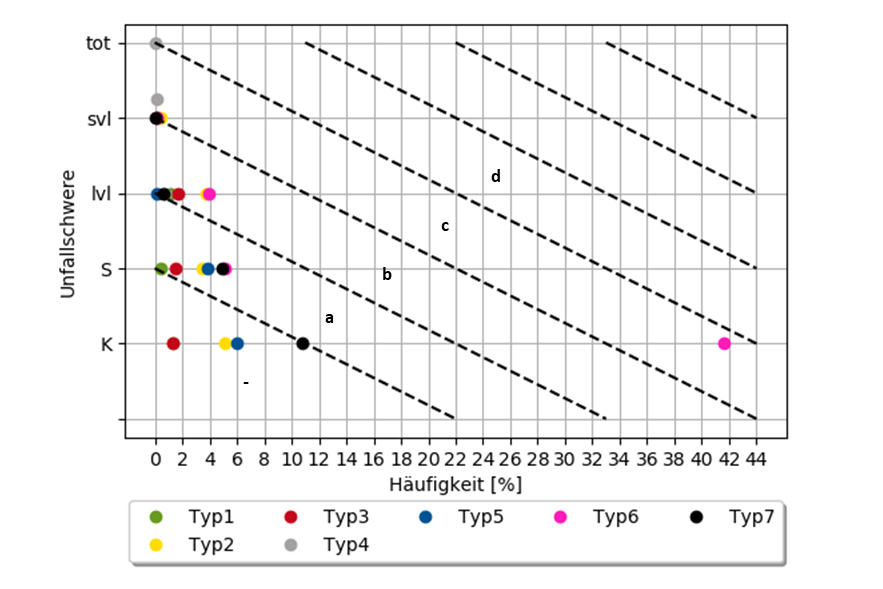
\includegraphics[width=12cm,height=8cm]{figures/Bewertung_UTF}
		\caption[Bewertung der Unfälle im Testgebiet anhand der sieben Unfalltypen mit Kleinunfällen]{Bewertung der Unfälle im Testgebiet anhand der sieben Unfalltypen mit Kleinunfällen}\label{fig:Bewertung_UTF}
	\end{figure}
\end{savenotes}

In die Kategorie \textit{c} fallen die Typen 1, 2, 3, 6 und 7 da hier jeweils Unfälle mit schweren Verletzungen auftraten. Abbildung \ref{fig:Bewertung_UTF(2)} im Anhang \ref{chapter:Bewertungsdiagramme} stellt vergrößerte Ausschnitte der Abbildung \ref{fig:Bewertung_UTF} zu besseren Verständlichkeit dar. Die Unfälle mit dem Typ 6 werden nicht nur aufgrund der Verletzungen mit der Kategorie \textit{c} bewertet, sondern auch aufgrund der hohen Anzahl, ca. 41,5 \%, an Kleinunfällen bei denen der Typ 6 angegeben wurde. Der Unfalltyp 5 wird, wie zuvor, mit der Kategorie \textit{b} bewertet.

Anhand der sieben Unfalltypen ist zwar eine Bewertung der Unfälle möglich, die Aussagekraft ist jedoch relativ gering, da der Unfalltyp wenig Informationen über den Unfallhergang preis gibt. Zur genaueren Beschreibung wurden die Feintypen nach GDV verwendet. Im Folgenden werden die sieben Unfalltypen anhand der aufgetretenen Feintypen analysiert. Aufgrund der hohen Anzahl der Feintypen werden nur die Unfälle denen die Risiko-Kategorie \textit{d}, \textit{c} oder \textit{b} zugeordnet wurde genauer beschrieben. Die restlichen Feintypen können aus den jeweiligen Diagrammen entnommen werden.

\subsubsection{Feintypen Unfalltyp 1}
Die zwei Feintypen 141 und 183 werden der Risiko-Kategorie \textit{c} zugeordnet, da es bei beiden zu Unfällen mit \ac{svl} kam. Typ 141 weißt eine höhere Anzahl an Unfällen mit \ac{svl} auf und zusätzlich kam es in 0,68 \% zu Unfällen mit \ac{lvl}, sodass die Unfälle mit \ac{lvl} die gleiche Risiko-Kategorie erreichen. Abbildung \ref{fig:Bewertung_FT1} stellt die Feintypen des Unfalltyps 1 dar. Die zugehörige Risiko-Kategorie kann anhand der Risikoäquivalenten (gestrichelte Linie) abgelesen werden.

\begin{savenotes}
	\begin{figure}[H]
		\centering
		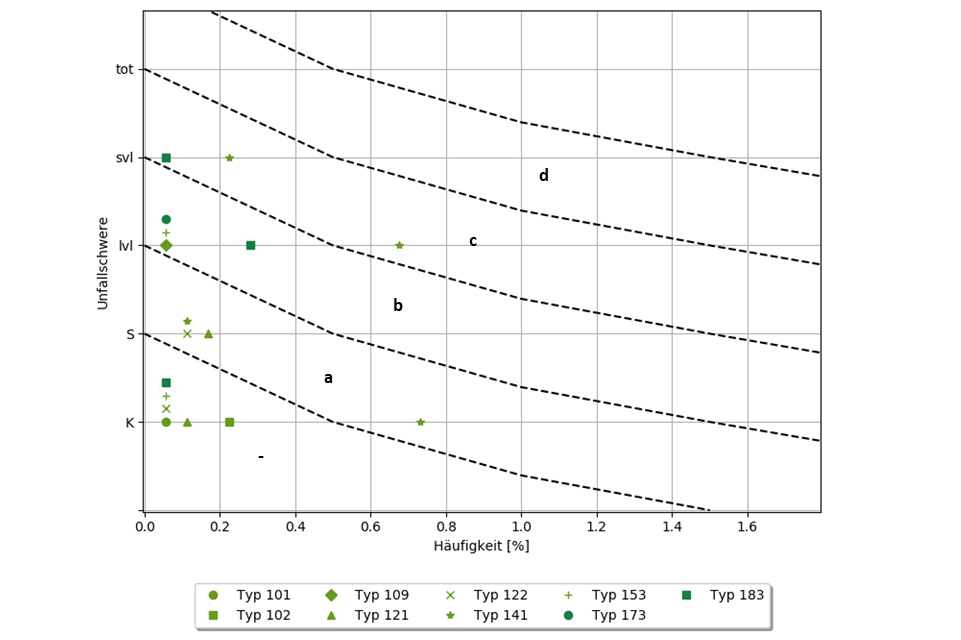
\includegraphics[width=12cm,height=8cm]{figures/Bewertung_FT1}
		\caption[Bewertung der Unfälle, denen ein Feintyp des Unfalltyps 1 zugeordnet wurde]{Bewertung der Unfälle, denen ein Feintyp des Unfalltyps 1 zugeordnet wurde}\label{fig:Bewertung_FT1}
	\end{figure}
\end{savenotes}

Der Risiko-Kategorie \textit{b} werden die Feintypen 109, 153 und 173 zugewiesen. Bei diesen drei Typen traten jeweils zwei Unfälle mit leicht Verletzten auf, die maßgebend für die Zuordnung der Risikokategorie sind. Um Feintypen mit gleicher Häufigkeit und gleicher Unfallschwere in den Diagrammen darstellen zu können wurden sie in der Höhe versetzt dargestellt.

\subsubsection{Feintypen Unfalltyp 2}
Betrachtet man Abbildung \ref{fig:Bewertung_FT2} ist zu erkennen, dass die Feintypen 211, 224, 243 und 244 der Risiko-Kategorie \textit{c} zugeordnet werden. Auffällig ist, dass alle vier Typen nicht nur aufgrund der Unfälle mit \ac{svl} in dieser Kategorie eingeordnet werden. Die Häufigkeit der Unfallanzahl mit \ac{lvl} ist bei allen vier Typen ebenfalls so hoch, dass sie in die Kategorie \textit{c} fallen. Besonders bei Typ 243 ereigneten sich mit 1,24 \% häufig Unfälle bei denen es zu \ac{lvl} kam. Bei Typ 211 kam es bei 0,96 \% ebenfalls zu \ac{lvl}. Zusätzlich ist bei Typ 211 auffällig, dass auch die Anzahl der Unfälle mit \ac{S} hoch ist. Sie beträgt 1,35 \% und befindet sich in der Risiko-Kategorie \textit{b} an der Grenze zu \textit{c}.

\begin{savenotes}
	\begin{figure}[H]
		\centering
		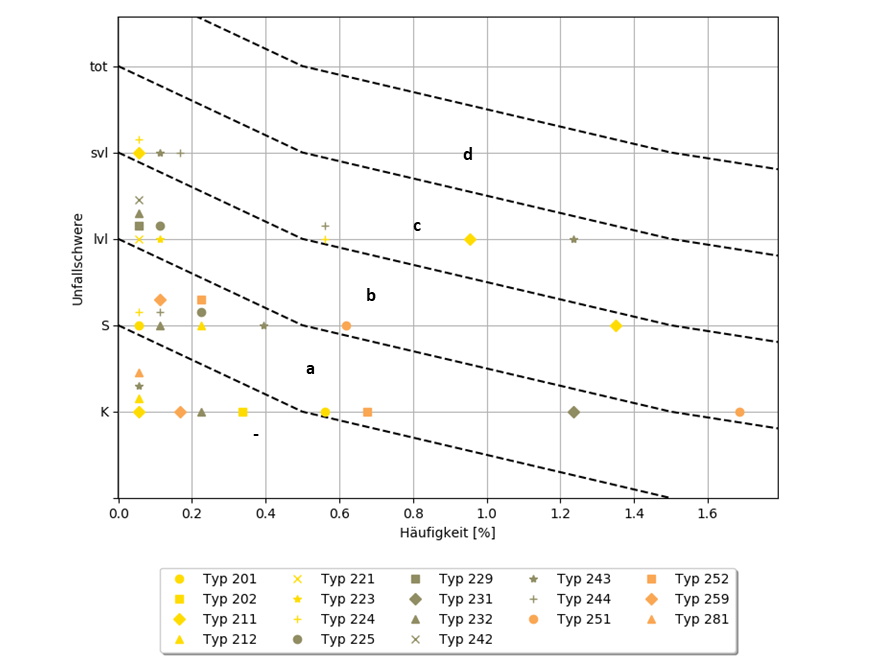
\includegraphics[width=12cm,height=8cm]{figures/Bewertung_FT2}
		\caption[Bewertung der Unfälle, denen ein Feintyp des Unfalltyps 2 zugeordnet wurde]{Bewertung der Unfälle, denen ein Feintyp des Unfalltyps 2 zugeordnet wurde}\label{fig:Bewertung_FT2}
	\end{figure}
\end{savenotes}

Den Feintypen 221, 223, 225, 229, 232, 242 und 251 wird die Risiko-Kategorie \textit{b} zugeordnet. Bis auf Typ 251 werden die Feintypen aufgrund der Anzahl der Unfälle mit \ac{lvl} dieser Kategorie zugeordnet. Bei Typ 251 ereigneten sich keine Unfälle, bei denen es zu einem Personenschaden kam. Die Anzahl der Unfälle mit \ac{S} und \ac{K} ist jedoch mit 0,62 \% bzw. 1,69 \% so hoch, dass der Feintyp ebenfalls in die Kategorie \textit{b} fällt.

\subsubsection{Feintypen Unfalltyp 3}
Der Risiko-Kategorie \textit{c} werden lediglich die Feintypen 342 und 349 des Unfalltyps 3 zugeordnet. In Abbildung \ref{fig:Bewertung_FT3} ist ersichtlich, dass beide Typen aufgrund der Unfallanzahl mit \ac{svl} dieser Kategorie zugewiesen werden. Bei dem Typ 342 ist die Häufigkeit der Unfälle mit \ac{lvl} mit 0,68 \% ebenfalls so hoch, dass diese auch in der Kategorie \textit{c} angeordnet werden.

Die Feintypen 301, 303, 322, 341 und 344 fallen alle in die Risiko-Kategorie \textit{b}, da es zu Unfällen mit \ac{lvl} kam. Am Häufigsten ereigneten sich solche Unfälle bei dem Typ 301 mit 0,23 \%.

\begin{savenotes}
	\begin{figure}[H]
		\centering
		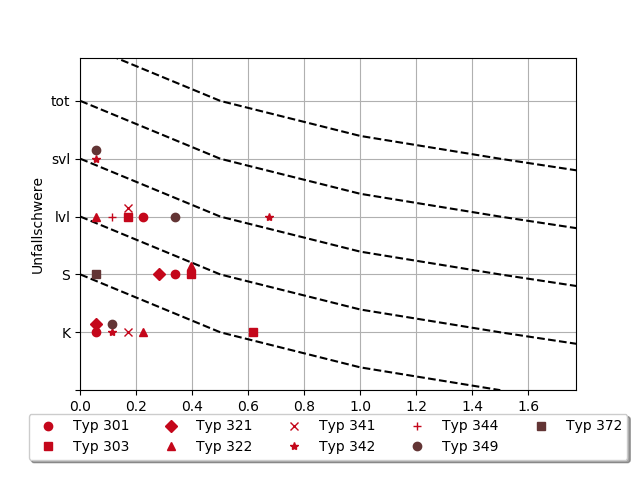
\includegraphics[width=12cm,height=8cm]{figures/Bewertung_FT3}
		\caption[Bewertung der Unfälle, denen ein Feintyp des Unfalltyps 3 zugeordnet wurde]{Bewertung der Unfälle, denen ein Feintyp des Unfalltyps 3 zugeordnet wurde}\label{fig:Bewertung_FT3}
	\end{figure}
\end{savenotes}

\subsubsection{Feintypen Unfalltyp 4}
Der Feintyp 401 erhält die Risiko-Kategorie \textit{d}. Diese Kategorie entspricht der höchsten Kategorie, die den Feintypen der Unfälle im Testgebiet zugeordnet wurde. Zusätzlich wird sie in dieser Arbeit nur bei zwei Feintypen angegeben. Der Feintyp 401 erhält diese Kategorie aufgrund der Unfallschwere. Allen betrachteten Unfällen, bei denen es zu einem tödlichen Unfall kam, wurde dieser Feintyp zugeordnet.

\begin{savenotes}
	\begin{figure}[H]
		\centering
		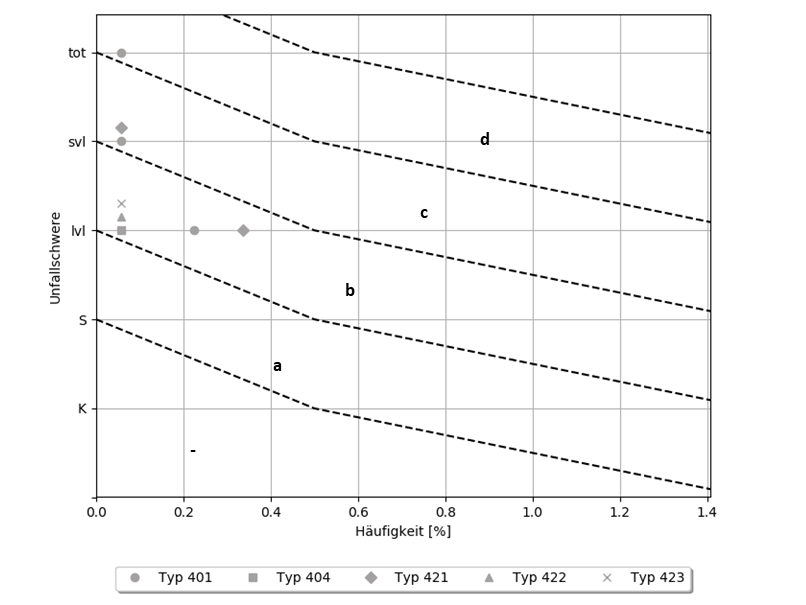
\includegraphics[width=12cm,height=8cm]{figures/Bewertung_FT4}
		\caption[Bewertung der Unfälle, denen ein Feintyp des Unfalltyps 4 zugeordnet wurde]{Bewertung der Unfälle, denen ein Feintyp des Unfalltyps 4 zugeordnet wurde}\label{fig:Bewertung_FT4}
	\end{figure}
\end{savenotes}

Der Risiko-Kategorie \textit{c} wurde, nur der Feintyp 421 zugeordnet. In Abbildung \ref{fig:Bewertung_FT4} ist zu erkennen, dass die Zuordnung der Kategorie aufgrund der Unfälle mit \ac{svl} erfolgt.

Die Feintypen 404, 422 und 423 erhalten die Risiko-Kategorie \textit{b}. Bei allen drei Feintypen ereignete sich je ein Unfall bei dem es zu leicht Verletzten kam. Häufiger traten leicht Verletzte bei den Feintypen 401 und 421 auf. Da diese aber bereits mit einer höheren Risiko-Kategorie bewerte wurden sind sie für diese Kategorie nicht mehr relevant.

\subsubsection{Feintypen Unfalltyp 5}
Neben dem eben erwähnten Feintyp 401 bildet der Feintyp 501 den zweiten Typ, dem die Risiko-Kategorie \textit{d} zugeordnet wird. Der Grund für eine Einordnung in diese hohe Kategorie stellt in diesem Fall allerdings nicht die Unfallschwere, sondern die Häufigkeit dar. In 3,49 \% wurde bei Unfällen mit schwerwiegendem Sachschaden der Feintyp 501 angegeben. Zusätzlich führte dieser Typ häufig zu Kleinunfällen. Diese sind jedoch mit 3,15 \% nicht maßgebend für die Kategorisierung.

Der Risiko-Kategorie \textit{c} wird hier kein Feintyp zugeordnet. In Abbildung \ref{fig:Bewertung_FT5} ist zu erkennen, dass in diesem Bereich lediglich der Feintyp 501 eingezeichnet ist. Diesem wurde bereits eine höheren Kategorie zugeordnet, somit ist er für diese nicht mehr relevant.

\begin{savenotes}
	\begin{figure}[H]
		\centering
		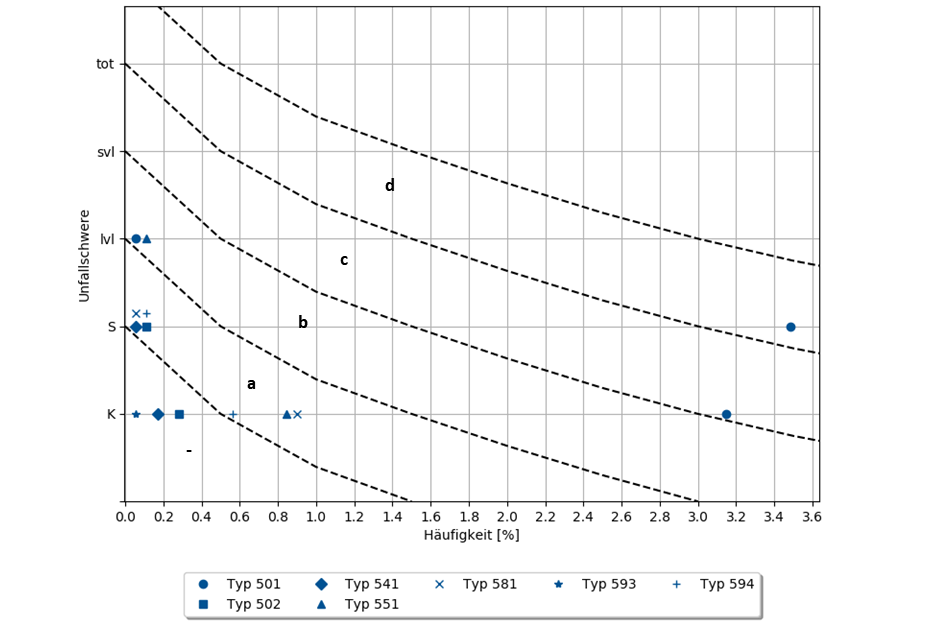
\includegraphics[width=12cm,height=8cm]{figures/Bewertung_FT5}
		\caption[Bewertung der Unfälle, denen ein Feintyp des Unfalltyps 5 zugeordnet wurde]{Bewertung der Unfälle, denen ein Feintyp des Unfalltyps 5 zugeordnet wurde}\label{fig:Bewertung_FT5}
	\end{figure}
\end{savenotes}

Der Feintyp 551 führte zu 2 Unfällen mit Leichtverletzten und erhält deshalb die Risiko-Kategorie \textit{b}. Allen anderen Feintypen des Unfalltyps 5 wurde eine niedrigere Kategorie zugeordnet. Sie werden daher hier nicht weiter erläutert.

\subsubsection{Feintypen Unfalltyp 6}
Betrachtet man Abbildung \ref{fig:Bewertung_FT6} ist zu erkennen, dass dem Unfalltyp 6 besonders viele Feintypen zugeordnet wurden. Deshalb stellt Abbildung \ref{fig:Bewertung_FT6(2)} in Anhang \ref{chapter:Bewertungsdiagramme} Teilbereiche der Abbildung \ref{fig:Bewertung_FT6} nochmals vergrößert dar.

Der Risiko-Kategorie \textit{c} wurden insgesamt acht Feintypen zugeordnet. Ein Feintyp stellt der Typ 63/64 dar. Dieser ist nicht im Unfalltypen-Katalog der GDV enthalten. Er wurde eingeführt um die Unfälle, die nicht typisiert werden konnten, zu reduzieren. Bei Kleinunfällen kommt es häufig vor, dass in den Kurzsachverhalten zwar angegeben wurde, dass der Unfall durch einen Fehler beim Spurwechsel entstand, es liegt jedoch keine Information über die Richtung des Spurwechsels vor. Bei allen Unfällen, denen der Feintyp 63/64 zugeordnet wurde, kam es daher entweder zu einem Fehler beim Spurwechsel nach rechts oder nach links. Diese Fehler spielen mit einer Häufigkeit von 6,63 \% bei \ac{K} eine bedeutende Rolle im Unfallgeschehen.

\begin{savenotes}
	\begin{figure}[H]
		\centering
		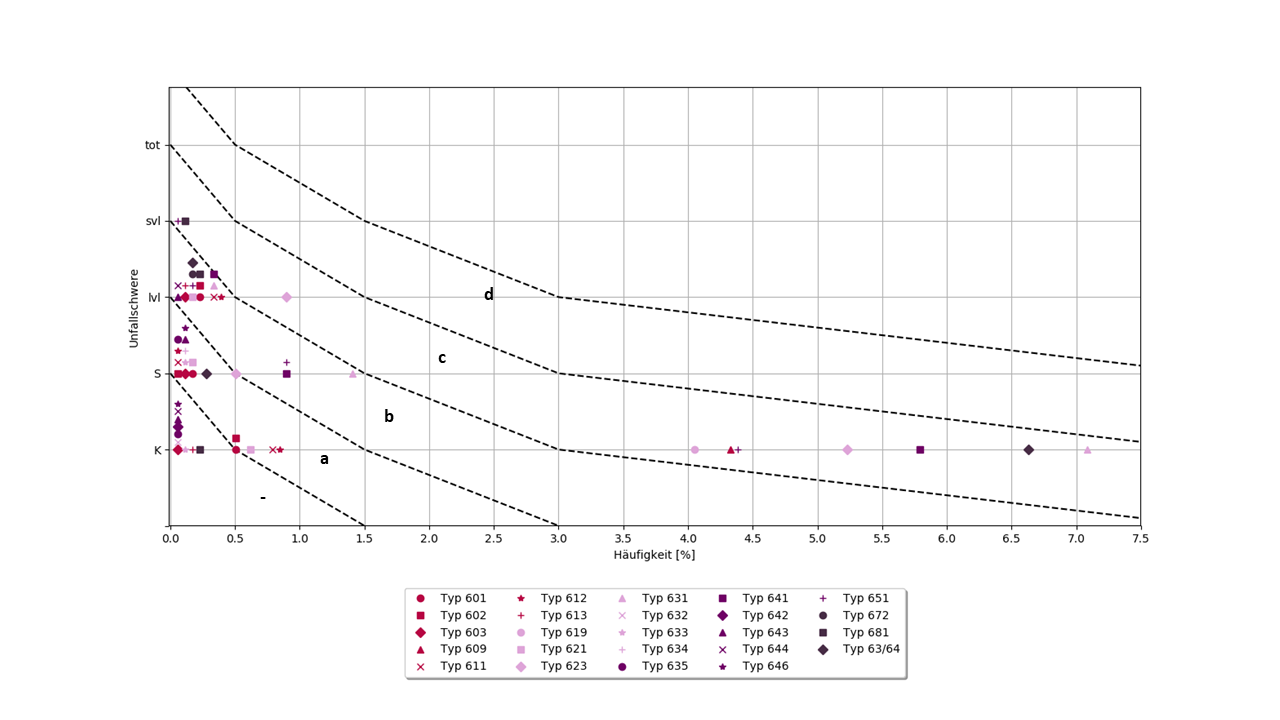
\includegraphics[width=18cm,height=10cm]{figures/Bewertung_FT6}
		\caption[Bewertung der Unfälle, denen ein Feintyp des Unfalltyps 6 zugeordnet wurde]{Bewertung der Unfälle, denen ein Feintyp des Unfalltyps 6 zugeordnet wurde}\label{fig:Bewertung_FT6}
	\end{figure}
\end{savenotes}

Lediglich bei Unfällen mit dem Feintyp 631 kam es mit 7,08 \% häufiger zu Kleinunfällen. Der Unfalltyp 641 führte in 5,79 \% zu Kleinunfällen und erhält daher ebenfalls die Risiko-Kategorie \textit{c}. Bei dem Feintyp 631 handelt es sich um Unfälle die durch einen Spurwechsel nach links entstanden sind. Der Feintyp 641 stellt die Unfälle beim Spurwechsel nach rechts dar. Laut Unfalltypen-Katalog werden diese beiden Typen angegeben, wenn der Spurwechsel aufgrund eines vorausfahrenden Fahrzeugs eingeleitet wird. In dieser Arbeit werden diese zwei Typen verwendet, sobald in den Kurzsachverhalten Fehler beim Spurwechsel nach links bzw. rechts angegeben wurden, da selten Informationen über den Grund des Fahrstreifenwechsels genannt werden.  

Die Feintypen 609, 619, werden ebenfalls aufgrund der hohen Anzahl an Kleinunfällen der Risiko-Kategorie \textit{c} zugeordnet. Bei den Feintypen 651 und 681 kam es zu Unfällen mit \ac{svl}, weshalb sie auch der Kategorie \textit{c} zugeordnet werden. Feintyp 651 weißt zudem eine hohe Anzahl an Kleinunfällen auf. Der Feintyp 623 wird sowohl aufgrund der Unfallanzahl mit \ac{lvl} als auch der Häufigkeit (5,23 \%) an Kleinunfällen der selben Kategorie zugeordnet.

Die Feintypen 601, 602, 603, 611, 612, 613 führten alle zu Unfällen mit \ac{lvl} weshalb ihnen die Risiko-Kategorie \textit{b} zugeordnet wurde. Ebenso die Feintypen 621, 643, 644 und 672. Feintypen denen aufgrund der Anzahl an Unfällen mit schwerwiegendem Sachschaden die Risiko-Kategorie \textit{b} zugeordnet wurde wurden alle schon in einer höheren Kategorie berücksichtigt.   

\subsubsection{Feintypen Unfalltyp 7}
Die Feintypen 701, 723 und 799 werden der Risiko-Kategorie \textit{c} zugeordnet. Der Typ 701 fällt vor allem aufgrund der Häufigkeit der Kleinunfälle (4,27 \%) aber auch aufgrund der Anzahl an Unfällen mit \ac{S} in diese Kategorie. Bei Feintyp 723 ist hingegen ausschlaggebend, dass es zu Unfällen mit \ac{svl} kam. Mit einer Häufigkeit von 1,52 \% bei den Unfällen mit \ac{S} zählt der Typ 799 schon knapp zur Kategorie \textit{c}.

\begin{savenotes}
	\begin{figure}[H]
		\centering
		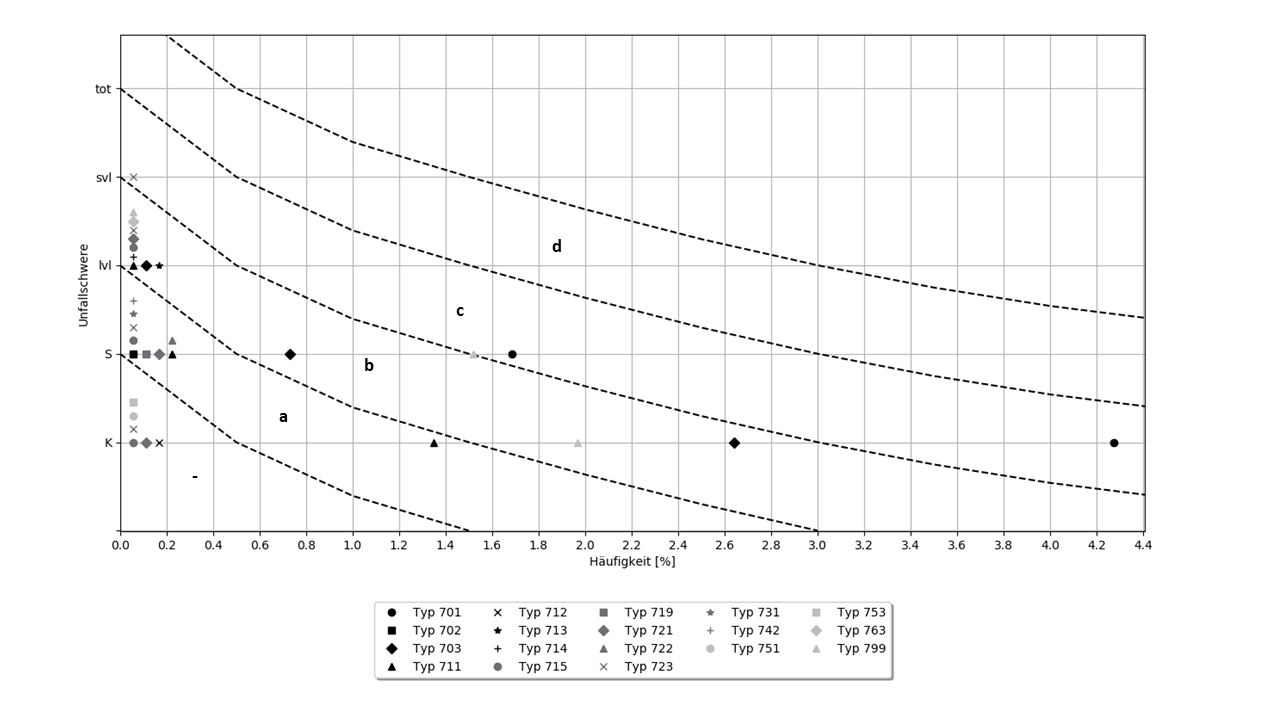
\includegraphics[width=18cm,height=10cm]{figures/Bewertung_FT7}
		\caption[Bewertung der Unfälle, denen ein Feintyp des Unfalltyps 7 zugeordnet wurde]{Bewertung der Unfälle, denen ein Feintyp des Unfalltyps 7 zugeordnet wurde}\label{fig:Bewertung_FT7}
	\end{figure}
\end{savenotes}

Der Feintyp 799 wird im Unfalltypen-Katalog mit \enquote{übrige Unfälle} bezeichnet. In dieser Arbeit wurde er immer dann angegeben, wenn anhand des vorhandenen Kurzsachverhalts kein anderer Feintyp zugeordnet werden konnte. Häufig handelt es sich hierbei um Unfälle mit festen Gegenständen (z.B. Lkw touchiert beim Abbiegen einen Ampelmast). Unfällen, bei denen die Kurzsachverhalte nicht aussagekräftig genug waren um den Unfallablauf annähernd zu verstehen, wurde in dieser Arbeit gar kein Feintyp zugeordnet. Theoretisch könnte ihnen auch der Typ 799 zugeordnet werden.   

Der Risiko-Kategorie \textit{b} wurden die Feintypen 703, 711, 713, 714, 715, 721 und 763 zugeordnet da es bei allen sieben Typen zu Unfällen mit leicht Verletzten kam. Lediglich der Typ 703 fällt zusätzlich noch mit einer Häufigkeit von 0,73 \% bei Unfällen mit \ac{S} und 2,64 \% bei Unfällen mit \ac{K} auf.

\section{Bewertung urbaner Fahrsituationen anhand der Feintypen}\label{section:Zuordnung der Unfälle zu Fahrsituationen}
Den Feintypen, die in Kapitel \ref{subsection:Bewertung der typisierten Unfälle} mit der Risiko-Kategorie \textit{b} oder höher bewertet wurden werden in diesem Kapitel beispielhafte Fahrsituationen zugeordnet. Das Vorgehen, welches angewendet wird um passende Situationen ausfindig zu machen wird in Kapitel \ref{subsection:Bewertungs urbaner Fahrsituationen} erläutert. Neben beispielhaften Fahrsituationen werden zusätzlich die Straßenbereiche angegeben, in denen es zu so einer Situation kommen kann. Es muss berücksichtigt werden, dass es sich dabei nur um Beispielsituationen handelt, die Fahrsituationen werden nicht vollständig beschrieben. Da das Verkehrsgeschehen im urbanen Raum sehr komplex ist muss berücksichtigt werden, dass sich auch bei nicht genannten Fahrsituationen Unfälle ereignen können, denen einer der beschriebenen Feintypen zugeordnet werden kann.

\subsection{Zuordnung mit Hilfe der aufgenommenen Fahrsituationen und den Kurzsachverhalten}\label{subsection:Zuordnung mit den aufgenommenen Fahrsituationen}
Den Feintypen werden beispielhafte Fahrsituationen zugeordnet, die bei Testfahrten im Untersuchungsgebiet aufgenommen wurden oder die sich aus den vorliegenden Kurzsachverhalten ergeben. Unter dem Begriff der Fahrsituation ist der aus Fahrersicht prinzipiell wahrnehmbare Ausschnitt der Verkehrssituation in Abhängigkeit des geplanten Fahrmanövers und des umgebenden Verkehrs zu verstehen. Zur besseren Verständlichkeit werden die Feintypen der sieben Unfalltypen, wie im vorherigen Kapitel, der Reihe nach betrachtet.

\subsubsection{Fahrsituationen zu den Feintypen des Unfalltyps 1}
Den Feintypen 141 und 183 wurde die Risiko-Kategorie \textit{c} zugeordnet. Sie können sich an vielen Stellen im Testgebiet ereignen und wurden daher bei den Testfahrten auch keiner speziellen Fahrsituation zugewiesen. Der Typ 141 kennzeichnet sich dadurch aus, dass der Fahrer während er auf einem geraden Straßenabschnitt fährt die Kontrolle über sein Fahrzeug verliert. Im Testgebiet kann sich diese Situation auf allen drei Straßen ereignen. Die Leopoldstraße weist im betrachteten Abschnitt einen geraden Verlauf auf. Auf der Ungererstraße ist nur der südliche Abschnitt durch eine Kurve geprägt. Die Schenkendorfstraße dagegen enthält weniger gerade Abschnitte. Die Auf- und Abfahrten zur A9 weißen Kurven auf, zusätzlich kommt es im Bereich des Petueltunnels zu Abschnitten mit Gefälle bzw. Steigung. Um Positionen zu bestimmen, an denen sich Unfälle mit diesem Feintyp ereigneten wird dieser in Kapitel \ref{section:Heatmaps} noch genauer betrachtet.

Unfälle mit dem Feintyp 183 ereigneten sich auf einem geraden Abschnitt mit einer Unebenheit. Dieser Typ wurde häufig bei Unfällen auf Radverkehrsanlagen angegeben. Hierbei kamen Radfahrer zum Sturz, weil sie den Randstein, der den Radweg vom Gehweg trennt, überfuhren. Im gesamten Testgebiet sind, von der Fahrbahn getrennte, Radverkehrsanlagen vorhanden. Dieser Typ kann sich daher auf allen Radwegen die außerhalb eines Knotenpunkts verlaufen ereignen. Auf der Leopoldstraße kommt es zudem in den Bereichen, in denen die Schienen der Tram gekreuzt oder auf der Fahrbahn geführt werden zu Unebenheiten. Des weiteren können Baustellen zu temporären Unebenheiten führen.

Feintypen, die der Risiko-Kategorie \textit{b} zugeordnet wurden stellen die Typen 109, 153 und 173 dar. Da es sich um Fahrunfälle handelt wurden auch hier während den Testfahrten keine beispielhaften Situationen aufgenommen. Der Feintyp 109 ereignet sich, wenn der Fahrer in Rechts- oder Linkskurven die Kontrolle über das Fahrzeug verliert. Diese Situation kann sich im Testgebiet vor allem in den Bereichen der Auf- bzw. Abfahrten zur A9 sowie im südlichen Bereich der Ungererstraße ereignen.

Verliert der Fahrer auf geraden Straßenabschnitten mit einem Gefälle oder einer Steigung die Kontrolle über sein Fahrzeug handelt es sich um den Feintyp 153. Dieser tritt im Testgebiet hauptsächlich im Bereich der Ein- bzw. Ausfahrt des Petueltunnels, sowie in den Bereichen der Auf- bzw. Abfahrten von der Schenkendorfstraße in Richtung Leopold- oder Ungererstraße auf.

Der Feintyp 173 wird angegeben, wenn sich ein Unfall aufgrund eines Engpasses auf einem geraden Straßenabschnitt ereignete. Diese Situation kommt in Testgebiet nur vor, wenn der Straßenquerschnitt aufgrund von Bau- oder Wartungsarbeiten verändert wird.

\subsubsection{Fahrsituationen zu den Feintypen des Unfalltyps 2}
Vier Feintypen des Unfalltyps 2 erhielten die Risiko-Kategorie \textit{c}. Bei drei Typen kam es jeweils zu Unfällen mit Radfahrern auf Radverkehrsanlagen. Lediglich der Feintyp 211 ereignete sich zwischen Fahrzeugen auf der Straße. Alle Unfälle, denen ein Feintyp des Unfalltyps 2 zugeordnet wurde ereigneten sich an einem Knotenpunkt. Abbildung \ref{fig:Knoten_Testgebiet} in Anhang \ref{chapter:Übersichtskarten} gibt einen Überblick über alle Knotenpunkte im Testgebiet. Bei dem Feintyp 211  kam es zu Unfällen zwischen Linksabbiegern und dem entgegenkommenden Geradeausverkehr. Bei den Testfahrten wurde diese Situation an der Einmündung Leopold-/Ungererstraße aufgenommen. Die Fahrsituation kann sich an allen Knotenpunkten im Testgebiet ereignen, bei denen Linksabbieger gleichzeitig mit dem Gegenverkehr grün erhalten. Diese Knotenpunkte wurden bereits in Kapitel \ref{subsechtion:Vorstellung der Teststrecke} analysiert. An Knotenpunkten mit einer eigenen Signalphase für Linksabbieger (vgl. Kapitel \ref{subsechtion:Abbiegeunfälle}) kann sich dieser Unfalltyp ereignen, wenn ein Unfallbeteiligter das Rotlicht missachtet hat oder es nicht möglich war, den Kreuzungsbereich rechtzeitig zu räumen.

Der Feintyp 224 stellt Unfälle zwischen Linksabbiegern und entgegenkommenden Radfahrern dar. Während den Testfahrten wurde diese Situation an den Knotenpunkten Leopold-/Ungererstraße und Leopold-/Rheinstraße aufgenommen. Da an allen Knotenpunkten im Testgebiet Radwege vorhanden sind kann sich diese Situation überall dort ereignen, wo es möglich ist nach links abzubiegen und beide Fahrströme gleichzeitig grün erhalten. Die Fahrsituation kann sich auch an Knotenpunkte eriegnen, die nicht signalisiert sind.. Ein Beispiel hierfür ist die Einmündung Ungerer-/Gundelindenstraße.

Während bis jetzt Situationen beim Linksabbiegen vorgestellt wurden kam es bei den Feintypen 243 und 244 zu Unfällen beim Rechtsabbiegen. Unfälle zwischen Rechtsabbiegern und Radfahrern, die in die gleiche Richtung fahren, wurden dem Feintyp 243 zugeordnet. Diese Situation wurde während der Testfahrten nicht aufgenommen. Sie kann sich an allen Knotenpunkten, mit und ohne LAS, im Testgebiet ereignen. Betrachtet man die Kurzsachverhalte ist die Einmündung Leopold-/Ungererstraße auffällig für solche Situationen.

Im Gegensatz zum Feintyp 243 kommt es beim Feintyp 244 nicht zu Unfällen mit Radfahrern, die sich in die gleiche Richtung bewegen, sondern mit entgegenkommenden Radfahrern. Auch hier wurde während den Testfahrten keine Situation aufgenommen, der dieser Feintyp zugeordnet wurde. Laut den Kurzsachverhalten kommt es an den Einmündungen Leopold-/Ungererstraße und Schenkendorf-/Lyonel-Feininger-Straße zu dieser Situation. Es muss berücksichtigt werden, dass sie sich theoretisch nur an Knotenpunkten ereignen kann, an denen es erlaubt ist den Radweg entgegen der Fahrtrichtung zu befahren. Da sich Radfahrer jedoch häufig nicht an die vorgegebene Fahrtrichtung halten muss auch an den anderen Knoten im Testgebiet mit dieser Fahrsituation gerechnet werden.

Sieben Feintypen des Unfalltyps 2 wurde die Risiko-Kategorie \textit{b} zugeordnet. Bei fünf handelt es sich dabei um Typen, denen Unfälle beim Linksabbiegen zugrunde liegen. Bei dem Feintyp 221 kommt es zu Unfällen mit Fußgängern, die sich in die gleiche Richtung wie das am Unfall beteiligte Fahrzeug bewegen. Während den Testfahrten wurde diese Situation an der Einmündung Leopold-/Ungererstraße aufgenommen. Diese Fahrsituation kann jedoch an allen Knotenpunkten auftreten, bei denen es möglich ist nach links abzubiegen. Zusätzlich müssen die querenden Fußgänger und die Linksabbieger gleichzeitig grün erhalten. An Knotenpunkten ohne \ac{LSA} kann es, sobald Linksabbiegen erlaubt ist, immer zu dieser Fahrsituation kommen.   

Dem Feintyp 223 liegt die gleiche Situation wie Typ 221 zugrunde. Es handelt sich jedoch anstelle der Fußgänger um Unfälle mit Radfahrern, die in die gleiche Richtung fahren. Zu dieser Situation wurde während den Testfahrten kein Beispiel aufgenommen. Auch hier müssen die Radfahrer und Linksabbieger gleichzeitig grün erhalten oder es handelt sich um einen Knoten ohne \ac{LSA}. Zusätzlich muss der Radweg theoretisch entgegen der Fahrtrichtung freigegeben sein. Hier greift jedoch wieder der Punkt, dass sich Radfahrer nicht immer an diese Regelung halten. Diese Fahrsituation kann sich z.B. erneut an der Einmündung Leopold-/Ungererstraße ereignen. Unfällen, bei denen unklar war, ob die Fußgänger bzw. Radfahrer sich entgegen der Fahrtrichtung oder in dieselbe Fahrtrichtung wie die Linksabbieger bewegten, wurde der Feintyp 229 zugeordnet. Es kann daher bei diesem Typ zu den oben beschriebenen Fahrsituationen des Unfalltyps 221, 223 oder 224 kommen.

Unfällen an denen eine Trambahn und ein Linksabbieger beteiligt waren wurde der Feintyp 225 zugeordnet. Diese Situation wurde ebenfalls nicht bei einer Testfahrt aufgenommen, kann sich jedoch nur im Bereich der Leopoldstraße ereignen. Innerhalb des Testgebiets kann die Tram in dem Bereich zwischen der Einmündung Leopold-/Ungererstraße und dem Schwabinger Tor beim Linksabbiegen gekreuzt werden. 

Einen weiteren Feintyp, bei dem es zu Unfällen mit Linksabbiegern kommt, stellt der Feintyp 251 dar. Er wurde den Unfällen zugeordnet, bei denen es zu einem Konflikt zwischen zwei nebeneinander fahrenden Linksabbiegern kam. Betrachtet man die Kurzsachverhalte ereigneten sich diese Unfälle überwiegend an den Knotenpunkten Leopold-/Schenkendorfstraße und Ungerer-/Schenkendorfstraße. Die Fahrsituation nebeneinander nach Linksabbiegen kann innerhalb des Testgebiets sonst nur noch an der Einmündung Leopold-/Ungererstraße auftreten.

Neben den fünf Feintypen bei denen es zu Unfällen mit Linksabbiegern kam wurde zwei Feintypen bei denen es zu Unfällen mit Rechtsabbiegern kam die Risiko-Kategorie \textit{b} zugeordnet. Einer davon ist der Feintyp 232. Hierbei kam es zu Konflikten zwischen Rechtsabbiegern und Radfahrern, die den Radweg in die gleiche Fahrtrichtung befuhren. Während der Testfahrten wurde keine Situation aufgenommen, die diesem Feintyp zugeordnet werden kann. Laut Kurzsachverhalten tritt sie vor allem an der Einmündung Leopold-/Ungererstraße auf. Innerhalb des Testgebiets kann es jedoch an allen Knotenpunkten zu dieser Fahrsituation kommen, da überall Radverkehrsanlagen vorhanden sind. An den lichtsignalisierten Knotenpunkten müssen die Rechtsabbieger und Radfahrer gleichzeitig grün erhalten damit diese Situation auftritt. Da es sich bei den Beteiligten um bedingt verträgliche Verkehrsströme handelt erhalten diese im Regelfall gleichzeitig grün.

Der Feintyp 242 beschreibt Konflikte mit Rechtsabbiegern und entgegenkommenden Fußgängern. Er wurde während den Testfahrten an den Knotenpunkten Ungerer-/Schenkendorfstraße, Leopold-/Ungererstraße, Leopold-/Potsdamerstraße und Leopold-/Karl-Theodorstraße aufgenommen. Diese Fahrsituation kann sich, aus den selben Gründen wie bei Feintyp 232, an allen Knotenpunkten im Untersuchungsgebiet ereignen. In Abbildung \ref{fig:Abbiege-Unfall} sind, bis auf Typ 251, alle Feintypen abgebildet.

\subsubsection{Fahrsituationen zu den Feintypen des Unfalltyps 3}
Der Unfalltyp 3 enthält mit den Feintypen 342 und 349 zwei Typen, denen die Risiko-Kategorie \textit{b} zugeordnet wurde. Während bei dem Feintyp 342 genau angegeben ist, dass es bei der Einfahrt in einen Knotenpunkt zu einem Konflikt mit einem wartepflichtigen Fahrzeug und einem Radfahrer von rechts kommt, ist bei Feintyp 349 unklar, auf welcher Straßenseite sich der Konflikt ereignet oder in welche Richtung der Radfahrer fährt. Diese Fahrsituation kann sich daher an allen Knotenpunkten im Testgebiet ereignen. Auffällig sind vor allem Knoten ohne \ac{LSA}. Abbildung \ref{fig:Einbiege-Unfall_Rad} stellt die Konfliktpunkte mit Radfahrern dar.

Der Feintyp 342 dagegen ereignet sich häufig an nicht signalisierten Einmündungen oder an Grundstücksein- bzw. Ausfahrten. Anhand der Kurzsachverhalte lassen sich zwei markante Punkte identifizieren an denen es zu dieser Fahrsituation kommt. Ein Punkt stellt die Einmündung Schenkendorf-/Lyonel-Feiniger-Straße dar, den Zweiten die Ausfahrt von der Aral-Tankstelle, die sich direkt neben der genannten Einmündung befindet. Bei diesen zwei Punkten ist der Radweg entgegen der Fahrtrichtung freigegeben. Es kann sein, dass die wartetepflichtigen Fahrzeugen nicht mit vorfahrtsberechtigten Radfahrern von rechts rechnen. Um weitere Punkte ausfindig zu machen, bei denen es aufgrund dieser Fahrsituation zu einem Unfall kam, wird der Feintyp 342 in Kapitel \ref{section:Heatmaps} berücksichtigt.

Fünf Feintypen erhielten die Risiko-Kategorie \textit{b}. Die zwei Feintypen 301 und 303 stellen einen Konflikt mit einem wartepflichtigen Fahrzeug und einem Fahrzeug das von links kommt dar. Bei Typ 301 hat der wartepflichtige die Absicht die Kreuzung geradeaus zu überqueren. Diese Fahrsituation wurde während den Tetfahrten nicht aufgenommen, kann sich jedoch nur an Kreuzungen ereignen. Da im Testgebiet nur signalisierte Kreuzungen vorhanden sind tritt diese Situation entweder dann auf, wenn es zu einem Rotlichtverstoß kommt oder der wartepflichtige Fahrzeugführer bei dichtem Verkehr bei grün in den Kreuzungsbereich einfährt, obwohl sich noch Fahrzeuge dort befinden. Er ist in dieser Situation verpflichtet zu warten, bis der Kreuzungsbereich geräumt ist.

Feintyp 303 stellt einen Konflikt zwischen einem wartepflichtigen Fahrzeug, das die Absicht hat nach rechts einzubiegen und einem Fahrzeug von links dar. Diese Fahrsituation kann sich an Kreuzungen und Einmündungen ereignen. An lichtisignalisierten Knoten müssen die gleichen Situationen berücksichtigt werden, die bereits bei Typ 301 angegeben wurden. Die Situation sollte daher eher selten an einem Knoten mit \ac{LSA} auftreten. Bei den Einmündungen ohne \ac{LSA} oder an Grundstückszufahrten kommt es jedoch häufiger zu solch einer Situation. Neben den beiden oben genannten Beispielen an der Schenkendorfstraße kann sich die Fahrsituation z.B. auch an der Einmündung Leopold-/Hörwarthstraße oder Ungerer-/Helmtrudenstraße ereignen.

Während bei den zwei Feintypen 301 und 303 Konflikte mit von links kommenden Fahrzeugen betrachtet werden kommt es bei dem Feintyp 322 zu einem Konflikt zwischen einem wartepflichtigen Linksabbieger und einem Fahrzeug von rechts. Diese Fahrsituation kann nur an Knoten auftreten, an denen das Abbiegen nach links möglich ist. Aufgrund der Grünstreifen zwischen den Fahrbahnen kommt diese Situation an Einmündungen ohne LSA im Bereich der Ungerer- und Leopoldstraße selten vor. Sie kann sich z.B. an den Einmündungen Ungerer-/Gundelindenstraße und Leopold-/Wilhelm-Hertz-Straße ereignen. Im Bereich der Schenkendorfstraße ist es an keiner Einmündung möglich nach links einzubiegen. Zusätzlich können sich solche Situationen auch an Knoten mit \ac{LSA}] ereignen. Hier liegt dann ein Rotlichtverstoß zugrunde oder das wartepflichtige Fahrzeug hat es den Fahrzeugen im Kreuzungsbereich nicht ermöglicht diesen zu räumen. Konflikte die sich zwischen zwei Fahrzeugen ereignen werden in Abbildung \ref{fig:Einbiege-Unfall} dargestellt.

Abschließen werden nochmal zwei Feintypen betrachtet, bei denen es zu Konflikten mit Radfahrern kommt. Der Feintyp 341 stellt einen Konflikt zwischen einem Fahrzeug, welches in den Knotenpunkt einfährt und einem Radfahrer von links dar. Diese Situation ereignet sich vor allem an nicht signalisierten Einmündungen. Hier müsste zusätzlich noch Berücksichtigt werden, ob der Radweg in beide Fahrtrichtungen freigegeben ist und auf welcher Seite sich die Einmündung befindet. Da Radfahrer den Radweg jedoch häufig entgegen der Fahrtrichtung befahren kann an allen Einmündungen mit dieser Fahrsituation gerechnet werden.

Der Feintyp 344 stellt einen Konflikt mit einem wartepflichtigen Fahrzeug, das den Knotenpunktbereich räumt und einem Radfahrer von rechts dar. Hierfür wurde während den Testfahrten ebenfalls keine beispielhafte Situation aufgezeichnet. Diese Fahrsituation kann sich jedoch nur an Kreuzungen ereignen. Da im Testgebiet nur Kreuzungen mit LSA vorhanden sind muss entweder ein Rotlichtverstoß vorliegen oder der Kreuzungsbereich wurde nicht geräumt. Bei hohem Verkehrsaufkommen kann es passieren, dass Radfahrer von rechts schon grün erhalten, während sich noch Fahrzeuge im Kreuzungsbereich befinden und diese geradeaus überqueren.

\subsubsection{Fahrsituationen zu den Feintypen des Unfalltyps 4}
Der Feintyp 401 wurde einem tödlichen Unfall im Testgebiet zugeordnet und deshalb mit der Risiko-Kategorie \textit{d} bewertet. Der Unfall mit Todesfolge ereignete sich im Bereich der Haltestelle Potsdamerstraße. Der Typ beschreibt Fahrsituationen, in denen Fußgänger von rechts vor einem Fahrzeug auf die Straße laufen. Diese Situation kann innerhalb des Testgebiets vor allem auf der Ungererstraße und der Leopoldstraße vorkommen. Die Richtungsfahrbahnen der Schenkendorfstraße sind baulich voneinander getrennt. Somit ist es nur schwer möglich, die Fahrbahn zu kreuzen. Auf der Ungererstraße kann sich diese Situation, bis auf den südlichen Bereich, hier ist ebenfalls eine Mitteltrennung vorhanden, auf der gesamten Straßenlänge ereignen. Betrachtet man den Straßenverlauf sind auf Google Maps teilweise hellere Stelle auf dem Grünstreifen zwischen den Fahrbahnen zu erkennen. Sie weisen, wie z.B. im Bereich der Einmündung Ungerer-/Hollandstraße, auf Fußgänger hin, die die Fahrbahn außerhalb von Knotenpunkten mit Querungshilfen überqueren. Auf der Leopoldstraße sind vor allem die Bereiche mit Haltestellen in der Mitte der Fahrbahn anfällig für diesen Feintyp. Im südlichen Teil ist es eher schwer, die Leopoldstraße außerhalb der Haltestellen oder Knotenpunkte zu queren, da sich in der Mitte der Fahrbahn das Rasengleis der Tram befindet. Im nördlichen Bereich sind Büsche auf dem Grünstreifen angeordnet, hier gibt es jedoch ebenfalls Lücken, die es ermöglichen die Fahrbahn zu überqueren.

In den oben genannten Bereichen kann es auch zu Unfällen kommen, denen der Feintyp 421 zugeordnet wurde. Er erhielt die Risiko-Kategorie \textit{c}. Hierbei handelt es sich um Fahrsituationen, die zu Konflikten mit kreuzenden Fußgängern von rechts führen. Des weiteren sind Situationen möglich, bei denen sich der Feintyp 422 (Kategorie \textit{b}) ereignet. Hierbei kommt der Fußgänger ebenfalls von rechts. Rechts neben dem Fahrzeug, mit dem es zum Konflikt kommt, befindet sich in diesem Fall jedoch ein weiteres Fahrzeug. Da die Richtungsfahrbahnen im Untersuchungsgebiet mindestens zwei Spuren aufweisen kann sich diese Fahrsituation ebenfalls in den oben genannten Bereichen ereignen.

Ein weiterer Feintyp, der Konflikte mit Fußgängern von rechts beschreibt und der ebenfalls der Risiko-Kategorie \textit{b} zugeordnet wurde, ist der Feintyp 423. Hier handelt es sich um eine Fahrsituation, bei der sich neben dem Fahrzeug mit dem es zum Konflikt kommt noch ein parkendes Fahrzeug befindet. Der Fußgänger tritt vor dem parkenden Fahrzeug auf die Straße und ist nur schwer zu erkennen. Diese Situation kann sich im Untersuchungsgebiet nur auf der Leopold- und Ungererstraße ereignen. Hier sind über den gesamten betrachteten Straßenverlauf Längsparkplätze auf beiden Straßenseiten vorhanden.

Dem Feintyp 404 liegt ein Konflikt mit Fußgängern von links zugrunde. Im Gegensatz zu dem Feintyp 401 befindet sich hier links neben dem Fahrzeug mit dem es zu Konflikt kommt ein weiteres Fahrzeug. Die Bereiche in denen es zu dieser Situation kommen kann stimmen jedoch mit denen des Typs 401 überein, da im Testgebiet überall zwei oder mehr Spuren je Richtungsfahrbahn vorhanden sind. 

\subsubsection{Fahrsituationen zu den Feintypen des Unfalltyps 5}
Dem Feintyp 501 wurde die Risiko-Kategorie \textit{d} zugeordnet. Hierbei handelt es sich um Unfälle die zwischen einem Fahrzeug, das sich auf der Straße im Längsverkehr bewegt und einem parkenden Fahrzeug entstehen. Bei den Testfahrten wurde dieser Feintyp vor allem Situationen in der Ungerer- und Leopoldstraße in den Bereichen mit Längsparkplätzen am Fahrbahnrand zugeordnet.  Zum Teil wurden auch Situationen mit Fahrzeugen, die in der zweiten Reihe parken/halten aufgenommen. Da auf der Schenkendorfstraße nur auf einem kurzen Abschnitt Längsparkplätze angeordnet sind ereignet sich diese Fahrsituation hier eher selten. Die Längsparkplätze in der Schenkendorfstraße sind direkt nach der Kreuzung mit der Leopoldstraße in Fahrtrichtung östlich angeordnet. Laut den Kurzsachverhalten kam es vor allem häufig zu Unfällen, bei denen der linke Außenspiegel der parkenden Fahrzeuge beschädigt wurde. Um markante Punkte im Testgebiet ausfindig zu machen, die anfällig für Unfälle sind denen diese Fahrsituation zugrunde liegt, wird sie in Kapitel \ref{section:Heatmaps} nochmal betrachtet.

In den oben genannten Bereichen mit Längsparkplätzen können sich auch Unfälle ereignen, denen der Feintyp 551 zugeordnet wurde. Er erhielt die Risiko-Kategorie \textit{b}. Während der Feintyp 501 Fahrsituationen darstellt, in denen sich das parkende Fahrzeug im Stillstand befindet, kommt es bei der Fahrsituation, die dem Feintyp 551 zugrunde liegt, zu Konflikten mit Fahrzeugen die Anfahren bzw. aus einem Längsparkplatz ausparken.

\subsubsection{Fahrsituationen zu den Feintypen des Unfalltyps 6}
Den Feintypen des Unfalltyps 6 wurde achtmal die Risiko-Kategorie \textit{c} zugeordnet. Zwei dieser Feintypen sind die Typen 609 und 619. Hierbei kommt es jeweils zu einem Auffahrunfall außerhalb von Knotenpunkten. Die neun am Ende der Nummer des Feintyps gibt an, dass die Spur, auf welcher sich der Unfall ereignete, unklar ist. Bei den Unfällen, die dem Feintyp 609 zugeordnet werden kommt es zu einem Auffahrunfall mit einem vorausfahrenden Fahrzeug im fließenden Verkehr. Unfälle, denen der Feintyp 619 zugeordnet wurde ereigneten sich aufgrund von Stau. Diese Fahrsituationen können sich im gesamten Testgebiet in allen Bereichen außerhalb von Knotenpunkten ereignen.

Im Gegensatz zu den oben beschrieben Feintypen ereigneten sich Unfälle, denen der Feintyp 623 zugeordnet wurde an Knotenpunkten. Hierbei kam es zu Auffahrunfällen zwischen einem Fahrzeug, das an einer roten Ampel anhält und einem oder mehreren nachfolgenden Fahrzeugen. Diese Fahrsituation kann sich an allen lichtsignalisierten Knotenpunkten im Untersuchungsgebiet ereignen.

Neben Auffahrunfällen ereigneten sich auch Unfälle beim Spurwechsel, denen die Feintypen 631, 641 und 63/64 zugeordnet wurden. Während es sich bei den ersten Unfalltypen um Unfälle handelt bei denen die Richtung des Spurwechsels bekannt ist (631: Fehler beim Spurwechsel nach links, 641: Fehler beim Spurwechsel nach recht) konnte den Unfällen, denen der Feintyp 63/64 zugeordnet wurde die Richtung des Spurwechsels nicht zugewiesen werden. Da die Fahrbahnen im Testgebiet durchgängig zwei oder mehr Fahrspuren enthalten kann es überall zu Fahrsituationen kommen, bei denen ein Fahrzeug die Spur wechselt. Spurwechsel können sowohl außerhalb, als auch im Bereich von Knotenpunkten durchgeführt werden.

Unfällen zwischen zwei Fahrzeugen, die nebeneinander fahren und bei denen keiner der Betroffenen die Absicht hatte die Spur zu wechseln, wurde der Feintyp 651 zugeordnet. Die Fahrsituation nebeneinander fahren, die diesem Typ zugrunde liegt kann sich ebenfalls im gesamten Testgebiet ereignen.

Bis jetzt wurden nur Feintypen betrachtet, bei denen es zu Unfällen zwischen nebeneinander oder hintereinander fahrenden Fahrzeugen kam. Der Feintyp 681 wurde Unfällen zugeordnet, bei denen es zu Konflikten mit entgegenkommenden Fahrzeugen kam. Die Fahrsituation begegnende Fahrzeuge sollte sich im Testgebiet lediglich auf den Radverkehrsanlagen ereignen, da auf der Straße im gesamten Gebiet Mitteltrennungen vorhanden sind. Trotzdem ist kann nicht ausgeschlossen werden, dass es auch auf der Straße zu solch einer Situation kommt, die z.B. durch eine Falschfahrer ausgelöst wird.

Die Risiko-Kategorie \textit{b} wurde zehn Feintypen des Unfalltyps 6 zugeordnet. Drei davon stellen die Feintypen 601, 602 und 603 dar. Hierbei kommt es wie bei Feintyp 609 zu Unfällen mit einem vorausfahrenden Fahrzeug im fließenden Verkehr. Die letzte Zahl des Feintyps gibt in diesem Fall jeweils die Fahrspur an, auf der sich der Unfall ereignete. Der ganz rechten Fahrspur wird dabei immer die Nummer eins zugeordnet. Da die Richtungsfahrbahnen im Testgebiet, auch außerhalb der Knotenpunkte, mindestens zwei Fahrstreifen aufweisen können Fahrsituationen, denen die Feintypen 601 und 602 zugrunde liegen überall auftreten. Zu Unfällen mit dem Feintyp 603 kann es dagegen nur innerhalb von Bereichen mit dreispurigen Richtungsfahrbahnen kommen. Solch eine Fahrsituation kann sich im nördlichen Bereich der Leopoldstraße und in Teilbereichen der Schenkendorfstraße ereignen. Auf der Schenkendorfstraße sind vor allem im Bereich der Auf- bzw. Abfahrt zur A9 drei oder mehr Fahrspuren vorhanden.

Die Feintypen 611, 612 und 613 können ebenfalls in den obengenannten Bereichen zu Unfällen führen. Die letzte Zahl der Nummer des Feintyps gibt auch hier wieder die Fahrspur an, auf der sich der Unfall ereignete. Im Vergleich zu den eben betrachteten Feintypen kommt es nun zu Auffahrunfällen zwischen einem Fahrzeug, dass im Stau steht und einem nachfolgenden Fahrzeug.   

Der Feintyp 621 stellt einen weiteren Typ dar, bei dem es zu einem Auffahrunfall kommt. Im Vergleich zu den oben genannten Feintypen ereignet sich dieser jedoch im Bereich eines Knotenpunktes. Es kommt zu einem Unfall zwischen einem wartepflichtigen Fahrzeug und dem folgenden Fahrzeug. Diese Situation wurde während der Testfahrten im Bereich der Einmündung Leopold-/Ungererstraße aufgenommen. Hier erhält der Linksabbieger grün, fährt in den Kreuzungsbereich ein, muss dann jedoch erneut anhalten um den vorfahrtsberechtigten Gegenverkehr passieren zu lassen. Ebenso sind Fahrzeuge, die die Leopoldstraße in nördliche Richtung befahren und nach rechts auf die Ungererstraße abbiegen gegenüber den kreuzenden Radfahrern wartepflichtig.

Bei den Feintypen 643 und 644 kommt es jeweils zu Unfällen beim Spurwechsel nach rechts. Dieser wird beim Feintyp 643 dadurch ausgelöst, dass die Fahrspur endet. Diese Fahrsituation kann sich im Testgebiet auf der Leopoldstraße in südlicher Fahrtrichtung im Bereich des Schwabinger Tors ereignen. Unfälle, denen der Feintyp 644 zugeordnet wurde, ereigneten sich aufgrund des Abbiegegeobts nach links. Sie kann sich an allen Knotenpunkten ereignen, die einen separierten Linksabbiegestreifen besitzen. Befindet sich ein Fahrzeug auf dem Linksabbiegestreifen, möchte die Kreuzung aber geradeaus überqueren, muss es die Fahrspur nach rechts wechseln. Diese Fahrsituation kann sich z.B. an den Knotenpunkten Leopold-/Schenkendorfstraße, Leopold-/Ungererstraße und Ungerer-/Schenkendorfstraße ereignen.

Während es bei den Feintypen die bis jetzt betrachtet wurden nur zu Unfällen zwischen Fahrzeugen kam wurde der Feintyp 672 Unfällen zwischen einem Fahrzeug und einem entgegenkommenden Fußgänger zugeordnet. Diese Fahrsituation kann sich vor allem auf der Leopold- und der Ungererstraße ereignen. Hier können die Fußgänger einfach auf die Straße laufen. Auf der Schenkendorfstraße ist dies nur erschwert möglich. Solche Fahrsituationen treten überwiegend in Bereichen mit Längsparkplätzen auf. Die Fußgänger laufen auf der Straßen, entlang der geparkten Fahrzeuge zu ihrem Fahrzeug oder zum nächsten Knotenpunkt. In den Kurzsachverhalten kam es auch zu Fällen, bei denen Fußgänger bewusst vor das Auto gelaufen sind um den Fahrer zu stoppen. In einem Fall lief der Fußgänger mit suizidaler Absicht vor ein Fahrzeug.

\subsubsection{Fahrsituationen zu den Feintypen des Unfalltyps 7}
Die drei Feintypen 701, 723 und 799 wurden mit der Risiko-Kategorie \textit{c} bewertet. Kam es bei Längsparkplätzen zu Unfällen zwischen einem ausparkenden und einem parkenden Fahrzeug wurde ihnen der Feintyp 701 zugeordnet. Diese Fahrsituation kann sich nur in den Bereichen des Testgebiets ereignen, in denen Längsparkplätze vorhanden sind. Diese kommen in der Leopold- und Ungererstraße wesentlich häufiger vor als in der Schenkendorfstraße. Während der Testfahrten wurde diese Fahrsituation nicht aufgenommen. Um Bereiche ausfindig zu machen, in denen diese Fahrsituation häufig vorkommt wird sie in Kapitel \ref{section:Heatmaps} nochmals betrachtet.

Bei Unfällen denen der Feintyp 723 zugeordnet wurde kam es zu einem Konflikt zwischen einem Fahrzeug das wendet und einem entgegenkommenden Fahrzeug. Die Richtungsfahrbahnen werden bei dieser Situation durch eine Mitteltrennung geteilt. Sie kann im Testgebiet vor allem an Stellen auftreten, an denen ein Wendehammer vorhanden ist, z.B. an der Kreuzung Leopold-/Schenkendorfstraße oder Ungerer-/Schenkendorfstraße. Zusätzlich ist es häufig erlaubt an Knotenpunkten zu wenden. Teilweise kommt es auch an Knotenpunkten mit Wendeverbot zu dieser Fahrsituation. Es muss daher an allen Knotenpunkten im Testgebiet damit gerechnet werden, dass diese Fahrsituation auftritt.

Der Feintyp 799 wird im Unfalltypen-Katalog mit \enquote{übrige Unfälle} bezeichnet. Ihm kann daher keine bestimmte Fahrsituation zugeordnet werden, weshalb er bei der Auswertung der Testfahrten gar nicht berücksichtigt wurde. In dieser Arbeit wurde er häufig bei Situationen angegeben, in denen es zu Unfällen mit festen Gegenständen kam, da diese in keinem anderen Unfalltyp berücksichtigt wurden. Solche Situationen ereigneten sich häufig im Bereich von Kreuzungen. Hierbei kam es z.B. vor, dass Lkws beim Abbiegen nach links oder rechts einen Ampelmasten touchierten. Auch Unfällen die dadurch entstanden, dass ein Fahrzeug rückwärts gegen einen festen Gegenstand, z.B. Straßenschild, fuhr wurde dieser Feintyp zugeordnet.

Die Risiko-Kategorie \textit{b} wurde sieben Feintypen des Unfalltyps 7 zugeordnet. Unfälle denen der Feintyp 703 zugeordnet wurde ereigneten sich auf einem Parkplatz. Hierunter fallen alle Fahrsituationen, die sich während dem aus- und einparken bzw. der Fahrt auf dem Parkplatzgelände ereignen. Diese Fahrsituationen wurden während der Testfahrten nicht aufgenommen, kommen innerhalb des Testgebiets aber z.B. auf dem Gelände von verschiedenen Tankstellen, Parkplätzen von Lebensmittelläden und öffentlichen Parkplätzen (z.B. Münchner Freiheit) bzw. Parkhäusern (z.B. Schwabinger Tor) vor.

Den Feintypen 711, 713, 714 und 715 liegen jeweils Unfälle, die sich beim Rückwärtsfahren ereigneten, zugrunde. Für alle vier Typen wurden keine Beispiele während der Testfahrten aufgenommen. Der Feintyp 711 beschreibt einen Konflikt mit einem Fahrzeug, welches rückwärts auf ein Fahrzeug auffährt, das sich direkt dahinter befindet. Diese Situation kommt laut den Kurzsachverhalten z.B. an Kreuzungen vor, wenn ein Fahrzeug zurücksetzt um die Spur zu wechseln. Bei dem Feintyp 713 tritt ein Konflikt mit einem rückwärts fahrenden Fahrzeug und einem kreuzenden Fußgänger auf. Diese Fahrsituation kann sich z.B. im Bereich von Grundstückszufahrten ereignen. Ein Fahrzeug fährt rückwärts aus der Zufahrt aus und übersieht dabei kreuzende Fußgänger auf dem Gehweg. Die Feintypen 714 und 715 beschreiben Situationen bei denen es zu Konflikten zwischen einem Fahrzeug das rückwärts fährt und einem weiteren Fahrzeug von rechts bzw. links kommt. Die Richtung wird immer aus der Perspektive des Fahrzeugs angegeben, welches den Konflikt verursacht. Hier also das, das rückwärts fährt. Diese Fahrsituation kann sich ebenfalls bei der Ausfahrt von Privatgrundstücken ereignen. Zudem kann es zu dieser Fahrsituation kommen, wenn Fahrzeuge rückwärts aus einem Knotenpunktarm in den Knoten einfahren. Dies ist z.B. an kleineren Einmündungen in Wohngebieten denkbar. Der Fahrzeugführer fährt z.B. rückwärts um zu wenden oder um einem anderen Fahrzeug Platz zu machen.

Der Feintyp 721 wurde ähnlich wie Feintyp 723 Unfällen, die sich bei Wendevorgängen ereigneten, zugeordnet. Hierbei entsteht jedoch kein Konflikt mit einem entgegenkommenden Fahrzeug, sondern mit einem Fahrzeug, das in die gleiche Richtung fährt und sich links neben dem Fahrzeug befindet, welches den Wendevorgang einleitet. Da im Untersuchungsgebiet nur mehrspurige Fahrbahnen vorhanden sind kann sich diese Fahrsituation an den Stellen ereignen, die bereits bei dem Feintyp 723 angegeben wurden.

Der Feintyp 763 wurde bei Unfällen angegeben, die durch plötzliches körperliches Unvermögen verursacht wurden. Dabei handelt es sich nicht um einen Schwächeanfall, der Fahrer ist nicht eingeschlafen und stand nicht unter Alkoholeinfluss. Diese Situation kann sich an jedem Punkt im Untersuchungsgebiet ereignen, da sie lediglich von der Fahrtüchtigkeit des Fahrers abhängig ist.

\subsection{Zuordnung mit Hilfe von Heatmaps}\label{section:Heatmaps}
Eine Heatmap ermöglicht es auffällige Punkte im Testgebiet bildlich darzustellen. Es werden alle Punkte, an denen es zu einem Unfall mit einem bestimmten Feintyp kam, markiert. Die Farbintensität nimmt mit der Häufigkeit der Unfallanzahl zu. Punkte, an denen häufig Unfälle auftreten sind rot markiert. Stellen an denen es seltener nur Unfällen kommt blau.

Betrachtet man die Heatmap in Abbildung \ref{fig:Heatmap_141} ist der Bereich an der Einmündung Leopold-/Ungererstraße orange gefärbt. Hier kommt es innerhalb des Testgebiets am häufigsten zu Unfällen mit dem Feintyp 141. Des weiteren ist zu erkennen, dass sich solche Unfälle hauptsächlich auf der Leopoldstraße ereignen. Die Leopoldstraße weißt einen geraden Straßenverlauf auf, der Voraussetzung für Unfälle mit dem Feintyp 141 ist. Zusätzlich hat \Textcite[S. 20]{Bruhn.2018} in seiner Arbeit festgestellt, dass es hier häufig zu Geschwindigkeitsüberschreitungen kommt. Erhöhte Geschwindigkeit kann dazu führen, dass der Fahrzeugführer die Kontrolle über sein Fahrzeug verliert. Der Kontrollverlust liegt allen Unfällen des Feintyps 141 zugrunde. Insgesamt ereigneten sich 31 Unfälle mit dem Feintyp 141, sechzehn davon auf der Leopoldstraße. Auf der Ungererstraße kam es nur zu fünf Unfällen mit diesem Feintyp. Dies kann daran liegen, dass hier das Verkehrsaufkommen geringer ist (vgl. Kapitel \ref{subsechtion:Unfälle während der HVZ}). Auf der Schenkendorfstraße kam es zwar mit zehn Unfällen ebenfalls seltener zu solchen Unfällen, es muss allerdings berücksichtigt werden, dass der betrachtete Abschnitt etwas kürzer ist als der, der Leopoldstraße (vgl. Tabelle \ref{tab:teststecke}).

\begin{savenotes}
	\begin{figure}[H]
		\centering
		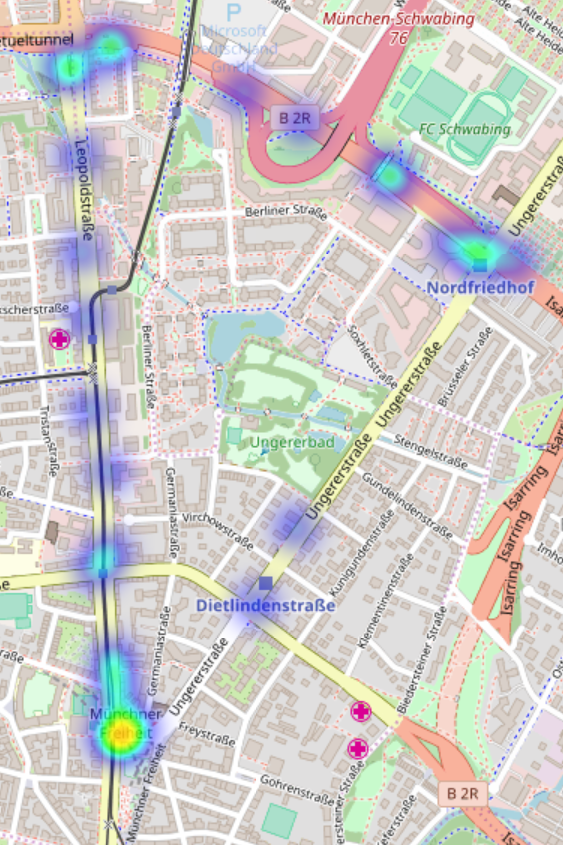
\includegraphics[width=9cm,height=12cm]{figures/HM_141}
		\caption[Heatmap der Unfälle mit dem Feintyp 141]{Heatmap der Unfälle mit dem Feintyp 141}\label{fig:Heatmap_141}
	\end{figure}
\end{savenotes}

Innerhalb des Untersuchungszeitraums wurde bei fünfzehn Unfällen der Feintyp 342 angegeben. Diese sind in Abbildung \ref{fig:Heatmap_342} dargestellt. Es ist deutlich zu erkennen, dass die Einmündung Schenkendorf-/Lyonel-Feininger-Straßen sowie die Ausfahrt der Aral-Tankstelle die direkt daneben liegt bei diesem Feintyp einen Unfallschwerpunkt darstellen. 73 \% der Unfälle mit dem Feintyp 342 ereigneten sich in diesem Bereich. Auf der Schenkendorfstraße kam es nur noch im Bereich der Einmündung zur Theodor-Dombart-Straße zu zwei weiteren Unfällen mit diesem Feintyp. Auf der Leopoldstraße ereigneten sich insgesamt nur zwei Unfällen und auf der Ungererstraße gar keiner. Die markanten Punkte, an denen sich diese Fahrsituation am häufigsten ereignete, wurden in Kapitel \ref{subsection:Zuordnung mit den aufgenommenen Fahrsituationen} bereits beschrieben. Hier konnten auch anhand der Heatmap keine weiteren markanten Stellen ausfindig gemacht werden.

\begin{savenotes}
	\begin{figure}[H]
		\centering
		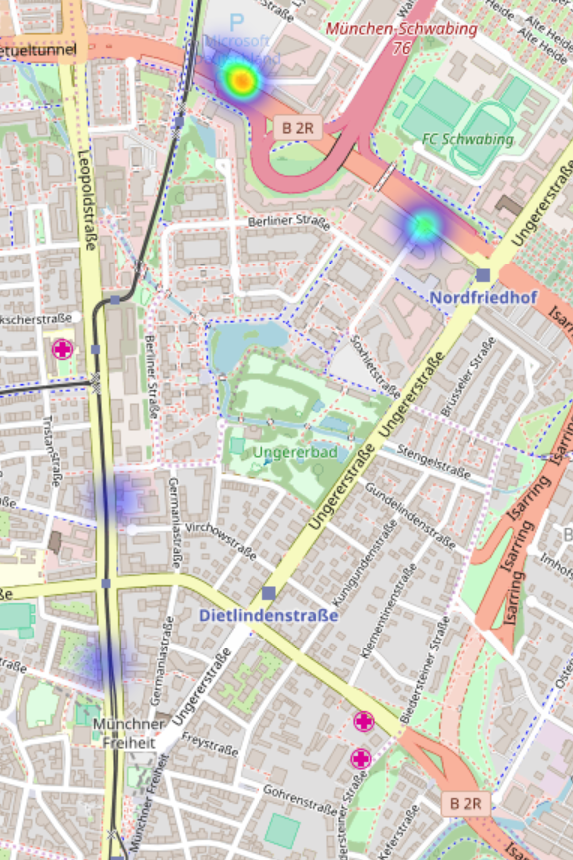
\includegraphics[width=9cm,height=12cm]{figures/HM_342}
		\caption[Heatmap der Unfälle mit dem Feintyp 342]{Heatmap der Unfälle mit dem Feintyp 342}\label{fig:Heatmap_342}
	\end{figure}
\end{savenotes}

Der Feintyp 501 wurde bei 119 Unfällen angegeben. Viele davon ereigneten sich, wie in Abbildung \ref{fig:Heatmap_501} zu erkennen ist im südlichen Bereich der Leopoldstraße. Hierbei kam es in nördliche Fahrtrichtung etwas häufiger zu Unfällen mit Fahrzeugen am Fahrbahnrand als in Südliche. Auf der Ungererstraße ereigneten sich ebenfalls mehr Unfälle im südlichen Bereich der Straße. Im Vergleich zur Leopoldstraße sind diese jedoch relativ gleichmäßig auf die entgegengesetzten Fahrtrichtungen verteilt. Auffällig ist, dass es auf der Ungererstraße einen weiteren Bereich gibt, in dem häufig Unfälle mit dem Feintyp 501 auftraten. Dieser liegt zwischen der Kreuzung mit der Soxhletstraße und der Einmündung zur Hollandstraße. Während die Unfälle im südlichen Bereich etwas verteilt entlang der Straße auftreten häufen sie sich in dem Zweiten an einer Stelle.

\begin{savenotes}
	\begin{figure}[H]
		\centering
		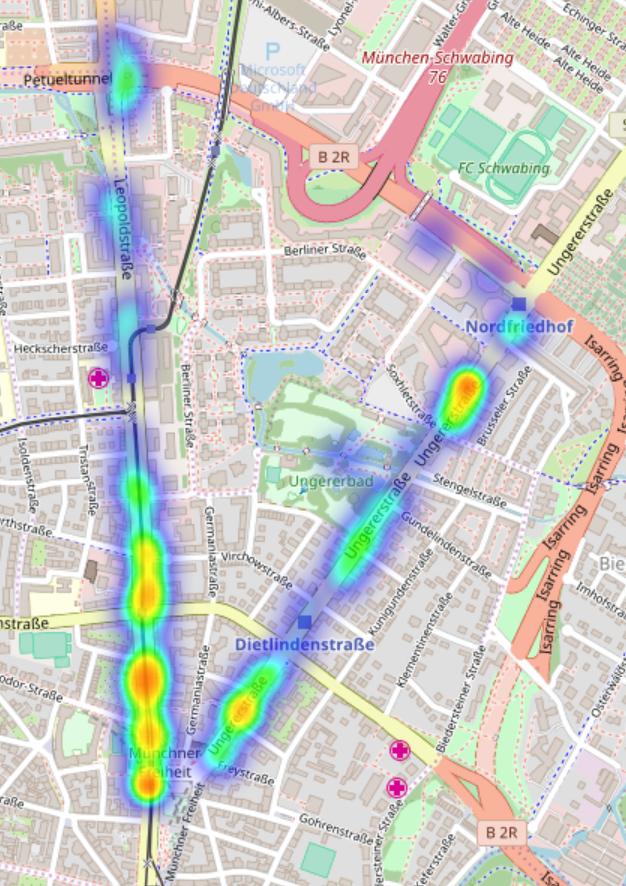
\includegraphics[width=9cm,height=12cm]{figures/HM_501}
		\caption[Heatmap der Unfälle mit dem Feintyp 501]{Heatmap der Unfälle mit dem Feintyp 501}\label{fig:Heatmap_501}
	\end{figure}
\end{savenotes}

Während der Feintyp 501 einen Konflikt zwischen einem Fahrzeug im fließenden Verkehr und einem haltenden/parkenden Fahrzeug darstellt. Beschreibt der Feintyp 701 einen Konflikt zwischen zwei parkenden Fahrzeugen. Genauer gesagt zwischen einem ein- bzw. ausparkenden und einem parkenden Fahrzeug. Da es bei beiden Feintypen zu Unfällen mit parkenden Fahrzeugen kam ähneln sich die erstellten Heatmaps. Insgesamt wurde der Feintyp 701 bei 106 Unfällen im Testgebiet angegeben, die in der Abbildung \ref{fig:Heatmap_701} dargestellt werden. Davon ereigneten sich lediglich zwei Unfälle auf der Schenkendorfstraße. Auf der Ungererstraße kam es zu 40 Unfällen. Hier ist vor allem der Bereiche zwischen der Fuchsstraße und Antonienstraße auffällig. In diesem Bereich befindet sich ein Lebensmittelgeschäft, die Fahrzeuge parken hier nur für eine kurze Dauer. Die hohe Anzahl der Unfälle in diesem Bereich kann durch die häufigen Ein- und Ausparkvorgänge erklärt werden. Die Unfälle die sich auf der Leopoldstraße ereigneten sind recht gleichmäßig über den Verlauf der Straße verteilt. Lediglich im nördlichen Teil kam es seltener zu Unfällen mit diesem Unfalltyp. Grund für die höhere Anzahl und gleichmäßigere Verteilung könnte sein, dass mehr gewerblich genutzte Flächen vorhanden sind. Diese haben einen höheren Wechsel der parkenden Fahrzeuge zur Folge. Die Bereiche in der Ungererstraße hingegen weißen überwiegend Wohnnutzung auf. Hier ist die Parkdauer der Fahrzeuge in der Regel länger, was zu einer geringeren Anzahl an Unfällen führt. 

\begin{savenotes}
	\begin{figure}[H]
		\centering
		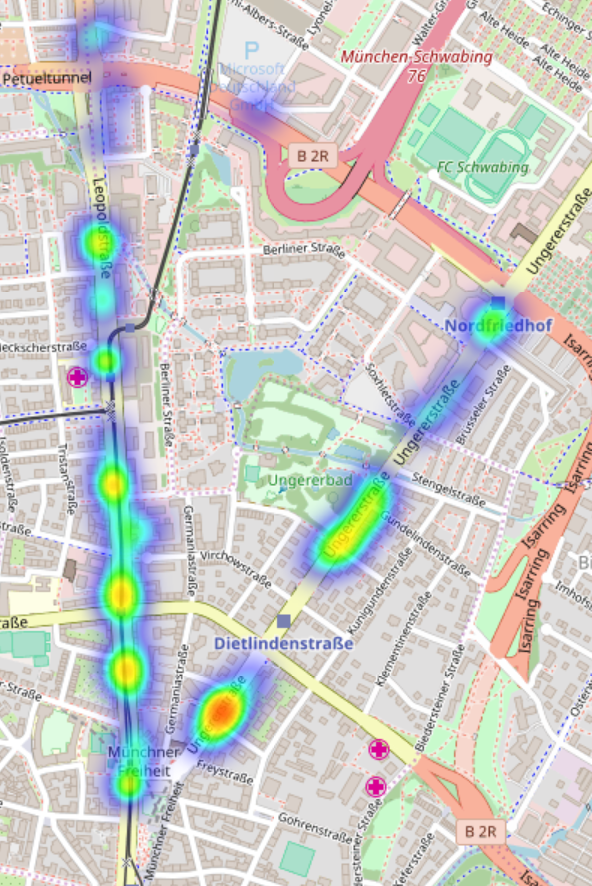
\includegraphics[width=9cm,height=12cm]{figures/HM_701}
		\caption[Heatmap der Unfälle mit dem Feintyp 701]{Heatmap der Unfälle mit dem Feintyp 701}\label{fig:Heatmap_701}
	\end{figure}
\end{savenotes}

Neben den vier vorgestellten Feintypen wurde achtzehn weiteren die Risiko-Kategorie \textit{c} oder höher zugeordnet. Diese wurden alle in einer eigenen Heatmap dargestellt und sind als html-Datei auf der im Anhang befindlichen CD zu finden. Die acht Feintypen 211, 224, 243, 244, 623, 631, 641 und 651 werden zusätzlich noch in Anhang \ref{chapter:Heatmaps} dargestellt. Diese Feintypen wurden gewählt, da Unfällen mit dem Unfalltyp 2 bzw. 6 viele Feintypen zugeordnet wurden. Zudem wurden Unfälle beim Abbiegen (Unfalltyp 2) und Unfälle im Längsverkehr (Unfalltyp 6) schon in Kapitel \ref{sechtion:Überprüfung der Thesen} betrachtet.

Der Feintyp 211 wurde während den Testfahrten an der Einmündung Leopold-/Ungererstraße aufgenommen. Dieser Bereich ist auch in Abbildung \ref{fig:Heatmap_211} ist zu erkennen. Am häufigsten kam es zu solch einer Situation jedoch an den Knoten Leopold-/Potsdamerstraße und Ungerer-/Schenkendorfstraße. Hierbei ist auffällig, dass die Linksabbieger am Knoten Ungerer-/Schenkendorfstraße überwiegend in einer eigenen Phase geführt werden. Trotzdem kommt es zu Konflikten mit entgegenkommenden Fahrzeugen. Grund dafür können Rotlichtverstößen oder Fehlverhalten beim Räumen des Kreuzungsbereiches sein. Der Feintyp 224 tritt, wie in Abbildung \ref{fig:Heatmap_224} zu erkennen ist häufig an der Kreuzung Leopold-/Potsdamerstraße auf. Hier wurde die Fahrsituation auch während den Testfahrten aufgenommen. Abbildung \ref{fig:Heatmap_243} zeigt eine Heatmap mit den Orten, an denen es zu Unfällen mit dem Feintyp 243 kam. Hier ist die Einmündung Leopold-/Ungererstraße am auffälligsten. Unfälle mit dem Feintyp 244 ereigneten sich dagegen vermehrt an der Kreuzung Leopold-/Schenkendorfstraße. Dieser Feintyp wird in Abbildung \ref{fig:Heatmap_244} dargestellt.

Der Feintyp 623 beschreibt Auffahrunfälle an lichtsignalisierten Knotenpunkten. Laut Abbildung \ref{fig:Heatmap_623} traten solche Fahrsituationen vor allem an den Kreuzungen Leopold-/Schenkendorfstraße und Ungerer-/Schenkendorfstraße sowie an der Einmündung Leopold-/Ungererstraße auf. In Abbildung \ref{fig:Heatmap_631} sind alle Unfälle des Unfalltyps 631 eingezeichnet. Es ist zu erkennen, dass im Bereich der Schenkendorfstraße am häufigsten Fehler beim Spurwechsel nach links auftraten. Unfälle denen ein Fehler beim Spurwechsel nach rechts zugrunde liegt werden in Abbildung \ref{fig:Heatmap_641} dargestellt und ereigneten sich überwiegend auf der Schenkendorf- und Leopoldstraße. Zu Unfällen mit dem Feintyp 651 kam es laut Abbildung \ref{fig:Heatmap_651} auf allen drei Straßen im Testgebiet. Auffällig ist hier jedoch, dass es hauptsächlich im Knotenpunktbereich zu Konflikten zwischen zwei nebeneinander fahrenden Fahrzeugen kommt.

\section{Zwischenfazit}
Um Unfälle rekonstruieren zu können werden weit aus mehr Daten, als in dieser Arbeit zur Verfügung stehen, benötigt. Hier liegen nur allgemeine Unfalldaten wie z.B. Unfalltyp, Unfallart, Unfallursache, Charakteristik und Besonderheit der Unfallstelle und Angaben zu den Beteiligten vor. Diese Daten reichen für eine Klärung der Schuldfragen. Für die Unfallforschung sind darüber hinaus Daten des Unfallorts und des Unfallfahrzeugs, in denen z.B. die Reifenspuren oder Spuren am Fahrzeug angegeben werden von Bedeutung. Sie werden benötigt um genau ermitteln zu können, wie es zu einem Unfall kam \parencite[S. 28]{Burg.2017}. Je genauer der Unfallhergang beschrieben wird, desto mehr Informationen liegen vor und Fahrsituationen, die dem Unfall vorausgehen können genauer beschrieben werden. Im Verlauf dieser Arbeit variieren die angegebenen Daten bezüglich ihrer Informationsgenauigkeit, da die Kurzsachverhalte erst später zur Verfügung standen. Während der erste Abschnitt dieses Kapitels überwiegend ohne die Kurzsachverhalte aufgestellt wurde wurden diese ab Kapitel \ref{section:Bewertung der Unfälle im Testgebiet} durchgängig berücksichtigt. Durch den zusätzlichen Informationsgewinn liegen vor allem bei den Kleinunfällen zusätzliche Informationen zum Unfallablauf vor. Der erste Abschnitt dieses Kapitels könnte mit Hilfe der Kurzsachverhalte nochmals überarbeitet werden. So ist es, vor allem bei der Auswertung der Hypothesen, möglich weitere Unfälle zu berücksichtigen.

Häufig wurde neben dem Unfalltyp die Unfallursache zur Analyse verwendet. Hier muss berücksichtigt werden, dass häufig nicht nur eine Unfallursache, sondern verschiedene Rahmenbedingungen mit negativem Einfluss auf die Verkehrssituation vorliegen. Laut \Textcite[S. 149]{StatistischesBundesamt.2016} haben Unfälle im Schnitt 1,4 Ursachen. Die Hauptunfallursachen beim Fahrzeugführer sind Fehler beim Abbiegen, Wenden, Rückwärtsfahren sowie beim Ein- und Anfahren. Am Zweithäufigsten wird die Vorfahrt bzw. der Vorrang anderer missachtet. Fahrsituationen die bei den genannten Hauptunfallursachen auftreten sind in der Regel sehr komplex und fordern eine erhöhte Aufmerksamkeit des Fahrzeugführers. Häufig ist dieser in solchen Situationen überfordert und kann das geplante Fahrmanöver nicht richtig ausführen. Da diese Situationen überwiegend an Knotenpunkten auftreten kommt es dort vermehrt zu Unfällen. Während sich innerhalb des Testgebiets überwiegend Unfälle zwischen zwei Pkws ereignen, die häufig nur zu Sachschaden oder leichten Verletzungen führen, kommt es bei Unfällen mit ungeschützten Verkehrsteilnehmern zu schwereren Verletzungen. Die Art der Verkehrsbeteiligung spielt daher bei der Betrachtung verschiedener Fahrsituationen eine wichtige Rolle.

Bei den in Kapitel \ref{section:Zuordnung der Unfälle zu Fahrsituationen} erläuterten Fahrsituationen wurden zwei mit der Risiko-Kategorie \textit{d} bewertet. Diese zwei Situationen verdeutlichen, wie unterschiedlich die Folgen verschiedener Fahrsituationen sein können. Während eine Situation aufgrund der Unfallschwere mit der Kategorie \textit{d} bewerte wurde kam es bei der anderen lediglich zu einer geringen Anzahl an leicht Verletzten. Die Anzahl der Unfälle bei denen es zu einem Sachschaden kam war dagegen ausschlaggebend für die Einordnung in diese Risiko-Kategorie. Je nach Art der Fahrsituation sind zudem unterschiedliche Bereiche innerhalb des Gebiets anfälliger für Unfälle. In Bereichen, in denen Fußgänger einfach die Fahrbahn überqueren können besteht z.B. ein erhöhtes Risiko für Fahrsituationen mit Fußgängerbeteiligung.

Zusammenfassen lässt sich sagen, dass viele Faktoren berücksichtigt werden müssen um eine Fahrsituation bezüglich ihrer Kritikaliät zu bewerten. Wichtig ist, dass nicht nur die Situation selbst, sondern auch das Umfeld in dem sich die Situation ereignet und weitere mögliche Beteiligte herangezogen werden. Nur so lässt sich eine Situation genau beschreiben und mögliche Konfliktpunkte können berücksichtigt werden. Die vollständige Betrachtung ist auch für die Entwicklung automatisierter Systeme relevant. Fahrsituationen die ein erhöhtes Risiko mit sich bringen können auch mit Hilfe dieser Systeme nur dann entschärft werden, wenn diese überhaupt in Betracht gezogen werden.